\ProvidesFile{template.tex}
    [2013/04/16 v3.2013^^J%
     Template file for NDdiss2e class by Sameer Vijay and updated by Megan Patnott^^J]
\documentclass[noinfo,final,sort&compress]{nddiss2e}
% One of the options draft, review, final must be chosen.
% One of the options textrefs or numrefs should be chosen
% to specify if you want numerical or ``author-date''
% style citations.
% Other available options are:
% 10pt/11pt/12pt (available with draft only)
% twoadvisors
% noinfo (should be used when you compile the final time
%         for formal submission)
% sort (sorts multiple citations in the order that they're
%       listed in the bibliography)
% compress (compresses numerical citations, e.g. [1,2,3]
%           becomes [1-3]; has no effect when used with
%           the textrefs option)
% sort&compress (sorts and compresses numerical citations;
%           is identical to sort when used with textrefs)

\usepackage{bm} 
\usepackage{tikz}
\usetikzlibrary{shapes,arrows}
\usepackage{pdflscape}
\usepackage[version=3]{mhchem}
\usepackage{mathtools}
\usepackage{abraces}
\usepackage{threeparttable}
\usepackage{multirow}
\usepackage{dcolumn}
\usepackage[export]{adjustbox}
\usepackage{mathrsfs}
\usepackage{ragged2e}
\usepackage{csquotes}
\usepackage{adjustbox}

\newcommand{\degree}{\ensuremath{^\circ}}

\begin{document}

\frontmatter % All the items before the first chapter go in ``frontmatter''

\title{EXPLORATION OF INTERFACIAL THERMAL CONDUCTANCE OF GOLD NANOPARTICLES USING MOLECULAR DYNAMICS}
\author{Suzanne M. Neidhart}
\work{Dissertation}
\degaward{Doctor of Philosophy}
\advisor{J. Daniel Gezelter}
\department{Chemistry and Biochemstry}
\maketitle

%\copyrightholder{Suzanne M. Neidhart} 
%\copyrightyear{2018}           
%\makecopyright

\begin{abstract}
In this dissertation I present work on elucidating factors important to heat transport in gold nanostructures, particularly nanoparticles, examining the effect of particle size, ligand layer rigidity, and surface gold vibrational freedom. The interfacial thermal conductance of various particles, as well as the thermal conductivity of nanoarrays that are of interest to see trends in heat transport.
Direct simulations of interfacial thermal conductance of solvated gold nanoparticles using molecular dynamics were calculated. All particle simulations used the Langevin Hull method for non-periodic systems.

Experimental nanoparticles contain a moiety, or ligand layer, at the surface of each particle that prevents aggregation and is a result of the method used in the formation of the particles. This moiety is essential in controlling movement of heat from a particle to the surrounding media. In particular, the following study looks closely at how the rigidity of this ligand layer and the length of the ligand change thermal transport at the interface of the particle. This allows for further insight into the important factors for ligand and solvent interactions to optimize heat flow. Proposed mechanisms for heat transfer rely on two effects: the vibrational overlap of the materials at the interface and the density overlap of the same materials.

After finding no direct relationship for particle size with the ligand layer and the thermal transport, a simpler system was examined: bare nanoparticles in solvent.
The particles consist of nanospheres, icosahedra, and cuboctahedra. The latter two display facets that are common in many nanostructures due to their stability.
The interfacial thermal conductivity (G) of the particles was examined based on radius and particle type. The coordination of gold atoms at the particle surface, giving information about the vibrational freedom, displayed a slight correlation with G. This supports the proposed important factors for heat transport found in the ligand layer work.

Finally, the ideas from both prior works are combined to study $Au_{144}PET_{60}$ particles in isolation and in an array. These small particles ($r \approx 10$ \AA) have highly undercoordinated gold atoms within the ligand layer. The thermal conductivity of the composite material is predicted using the Hasselman and Johnson equation, which uses individual components of the composite systems, and compared to preliminary results for the simulated nanoarrays. In the predicted conductivity, the nanoarray thermal conductivity is highly dependent on the geometric feature, $v_p$, the particle volume fraction. 

\end{abstract}

% \renewcommand{\dedicationname}{NEW DEDICATION NAME}
% \begin{dedication}
% \end{dedication}

\tableofcontents
\listoffigures
\listoftables

%\begin{preface}
%\vfill
%\begin{flushright}
%\textit{''Some say the world will end in fire,} \\
%textit{Some say in ice.''}\\
%--Robert Frost
%\end{flushright}
%\vfill
%\end{preface}

\begin{acknowledge}
First, I would like to thank my advisor, Professor J. Daniel Gezelter, for his persitent guidance and support throughout this research. My time in graduate school has been greatly enriched by having such a wonderful mentor.
His patience for all the little questions and concern for the individual's growth has been unmatched.

I am grateful to my committee, Professor J. Daniel Gezelter, Professor Steven A. Corcelli, and Professor William F. Schneider for their insightful questions and helpful suggestions in navigating this research.
Additionally, I would like to thank Professor Christine M. Aikens for her continual mentorship and guidance during transition periods of my career.
I am grateful to past group members, especially Dr. Shenyu Kuang, Dr. Kelsey M. Stocker, Dr. Joseph R. Michalka, Dr. Madan Lamichhane, Dr. Patrick B. Louden, and Thomas Parsons for laying the foundations of the research, helpful conversations, and continuously challenging me to be a better scientist.
I am very thankful for the current group members, Hemanta Bhattarai, Alexander Mazanek, Cody Drisko, and Nicholas Milikich for the helpful discussions, research related and otherwise.
I would also like to acknowledge the Corcelli group, in particular Dr. Mary Sherman and Dr. Clyde A. Daly Jr., for their useful discussions and camaraderie. 

Throughout my time spent at Notre Dame, I have been blessed with great friendships that have made the path through graduate school brighter, that I would be remiss to not mention: Ruthie Nelson, Claire Bowen, Ju-Young Kim, Arielle Lopez, Rachel Miller, Madeline Smith, Jeremy Eberle, and Melissa Hofferbaur. 
In particular I would like to thank the Association for Women in Science, a group that created an instant community and through which I formed strong friendships.

In addition to all the above, I would like to acknowledge my family for their support throughout my life. 
Many thanks to my siblings, for all the phone calls, visits, and encouragement over the years.
And to my parents, for whom I would not be where I am today without their years of sacrifice and continued love and support.

Finally, I would like to thank my husband and best friend, Peter Neidhart. His support and understanding throughout our time at Notre Dame has been essential for the completion of this document, and he continues to bring happiness to my life. 
%
\end{acknowledge}

\mainmatter

%\bibpunct{[}{]}{,}{n}{,}{,}
%%%%%%%%%%%%%%%%%%%%%%%%%%%%%%%%%%%%%%%%%%%%%%%%%%%%%%%%%%%%%%%%%%%%%%%%%%%%%%%%%%%
%		CHAPTER 1 -- INTRODUCTION
%%%%%%%%%%%%%%%%%%%%%%%%%%%%%%%%%%%%%%%%%%%%%%%%%%%%%%%%%%%%%%%%%%%%%%%%%%%%%%%%%%%
\chapter{INTRODUCTION}\label{chap:intro}
This chapter explores the basics of heat transfer and molecular dynamics. The challenges existing in the current methods of finding transport quantities using molecular dynamics are included. Finally, applications of molecular dynamics to finiding thermal tranport in systems of interest are presented. The remaining chapters use the methods described here to examine systems of interest.

The first application, gold nanospheres of varying sizes and ligands, are presented in Chapter 2.  There are three different variables to characterize these systems: particle size, ligand length, and ligand rigidity. Through looking at the vibrational density of states and the density profiles for the systems, two important factors for heat transport can be determined: the vibrational overlap of the material at the interface and the physical proximity/overlap of the material at the interface. This information gives relevant principles for ligand and particle design, while no clear trend for particle radius was established. 

In an attempt to detangle the size and the ligand dependence, Chapter 3 takes a closer look at the particle surface and size dependence. 
The particles are left bare but have a range of sizes and three different geometries: spheres, icosahedra, and cuboctahedra.
The three different morphologies give  distinct vibrational spectra at the particle surface, allowing for different thermal conductivity. In addition to the particles, planar systems displaying the prominent facets of the particles were studied. This work suggests the need for a proximity factor contributing to a model of thermal transport.
The vibrational overlap of the material at the interface matters, but so does the amount of the material that is transferring heat. This is most clearly seen through the surface density of undercoordinated surface atoms in the planar systems.

Chapter 4 presents a combination of the concepts in the previous chapters through the study of small nanoparticles both in isolation and in a nanoarray. The $\ce{Au}_{144}\ce{PET}_{60}$ particle are approximately 9 \AA\ in radius and have a crystal structure found at very low temperatures which is an appropriate starting structure simulating heat transport in arrays. A unique aspect of these particles, and similar small structures, is that the ligand layer has gold atoms pulled away from the surface. This leads to lower coordination of the outer-most gold atoms, which now exhibit different vibrational spectra. These particles were simulated in two different solvents to observe solvent effects on the thermal conductivity of these particles.

Finally, Chapter 5 looks forward to potential applications of a new fluctuating charge embedded method to be applied to metal surfaces and particles in polarizable solvents. This new method would allow for the examination of charge effects on thermal transport and arrangement of solvent at the surface of the metal.

\section{Heat Transport}
The classical definition of temperature is a quantity that describes a thermal equilibration phenomena. At the macroscopic level, heat can be transferred in three ways: conduction, convection, and radiation.~~\cite{Chen2005} 
Under the equipartition theorem, where the average kinetic energy of a particle is \(\frac{3k_{B}T}{2}\), the temperature is a reporter of the kinetic energy of the system.~\cite{Goldstein2001}
When the kinetic energy is distributed evenly among all independent parts of the system, the heavy atoms in a system would have a small average speed than the lighter atoms in the system. 

On the microscopic level, heat moves through different paths depending on the composition of the system.~\cite{Chen2005}
In a gas, heat is transferred primarily through collisions, while in semiconductors thermal energy moves through the propagation of vibrations in the solid, ie. phonons. 
A phonon is a quantized lattice wave that traverses the material with a longitudinal or transverse polarization.~\cite{Kittel} 
In metals, where the material has a solid lattice embedded in a sea of electrons, both phonon and electron heat transfer contribute.~\cite{Kittel} 
Electrons in a metal system are typically treated as an electron gas.
Electrons travel at velocities that are approximately three orders of magnitude larger than phonons, therefore the electron contribution dominates heat transfer in metals and is important when considering bulk thermal conductance of metals.
At a metal/non-metal interface the thermal conductance through the non-metal is dominated by phonon scattering, rather than electronic contributions.~\cite{Chen2005, Cahill2011, Stoner1993}
%(All prior material is from Gang Chen Book)

\subsection{Heat Transfer at Interfaces}
Further examination of phonons as the only heat carriers can be done at the interface of two materials. If the phonon is traveling through material A and approaches material B with frequency $\omega$, with angles $\phi$ and $\theta$ normal to the interface; there is a transmission probability, $\tau_{a\rightarrow b}(\omega)$, that the wave will continue into material B (see Figure \ref{fig:interface-graphic}).~\cite{Monachon2016} 
The transmission probability must satisfy detailed balance.
%, meaning $\tau_{a\rightarrow b} = 1 - \tau_{b\rightarrow a}$
There are two major models that make predictions for heat transfer at the interface: the acoustic mismatch model (AMM) and the diffuse mismatch model (DMM).~\cite{Monachon2016}
\begin{figure}
    \centering
    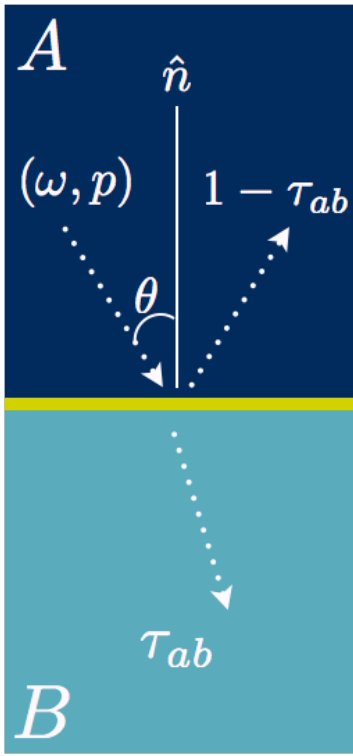
\includegraphics[scale=0.75]{figures/interface-graphic.png}
    \caption{Here an incoming phonon in material A is approaching the interface of materials A and B. The wave has a polarization ($p$) and frequency ($\omega$) and approaches the interface at an angle ($\theta$) relative to the normal of the interface. The phonon, under the DMM, has two options at the interface: scatter through to material B or scatter back through material A. The probability of transmission is given by $\tau_{ab}$. Due to detailed balance, the scattering back to material A is $1 - \tau_{ab}$.}
    \label{fig:interface-graphic}
\end{figure}

\subsection{Acoustic Mismatch Model}
In the acoustic mismatch model, the transmission probability- the total fraction of energy transmitted across the interface- is dependent on the acoustic impedance of the material, $Z_i$. The AMM evaluates the transmission coefficient through a continuum approach.~\cite{Little1959} This model uses the acoustic transmission and reflection between the two materials and ignores the granularity of the materials. Therefore the AMM would be most appropriate for low temperatures where the thermal spectrum is dominated by long wavelength phonons.~\cite{Graff1975} 

Each transmitted phonon has three possible polarizations: one longitudinal and two transverse. Likewise, reflected phonons can be reflected in the same fashion, giving six different paths for a wave to interact with the interface. This problem is usually simplified sing the acoustic analog of Snell’s law:
\begin{equation}
\tau_{ab}(\theta, p) = \frac{4\frac{p_2 \nu_{p, 2}}{p_1 \nu_{p,1}} \frac{\cos{\theta_{p,2}}}{\cos{\theta_{p,1}}}}{\big( \frac{p_2 \nu_{p, 2}}{p_1 \nu_{p,1}}+ \frac{\cos{\theta_{p,2}}}{\cos{\theta_{p,1}}}\big)^2}
\end{equation}
where $\theta$ are related to the analog of Snell's law through the frequency: \(\frac{\sin{\theta_1}}{\nu_1} = \frac{\sin{\theta_2}}{\nu_2}\).

Transmission can be simplified using acoustic impendances:
\begin{equation}
\tau_{ab}(\theta, p) = \frac{4Z_a Z_b}{(Z_a +Z_b)^2}
\end{equation}
where $Z$ is the acoustic impedance of each material, $Z_a = \rho_a v_a$, which depends on, $\rho$, the density and $v$, the speed of sound in the material. 

More complex treatments of the sound waves~\cite{Prasher2000} and treatments accounting for the interfacial bonding~\cite{Prasher2009} through the AMM have been studied. These modifications result in values that are lower than traditional AMM, therefore much below the experimental measurements of the systems.~\cite{Cahill2006, Stoner1993}

\subsection{Diffuse Mismatch Model}
The diffuse mismatch model assumes that the phonon has two options when the wave meets the interface: the phonon can transfer into material B or be reflected back into material A (see Figure \ref{fig:interface-graphic}). It operates under the assumption that all phonons at the interface are scattered randomly, meaning that all memory of the direction and polarization are lost. The phonon only keeps the frequency constant during the interaction of the two materials, hence all probability of the phonon to propagate into a material is dependent of the material's density of states. 

Under the DMM, the thermal conductance at an interface between $a$ and $b$ can be approximated,  
\begin{equation}
G_{ab} = \frac{1}{4 \pi} \sum_p \int_\omega \int_\theta \int_\phi \hbar \omega \frac{\partial f}{\partial T}  v_a  \rho_a  \tau_{ab} \cos\theta \sin\theta d\theta d\phi d\omega
\end{equation}
where $f$ is the Bose-Einstein distribution function, $v_a(\omega, p)$ is the group velocity (on side $a$) for a phonon characterized by frequency $\omega$, moving in direction ($\theta, \phi$) with polarization $p$.  The relevant material properties are the density of phonon states, $\rho_a(\omega, p)$, and the transmission probability, $\tau_{ab}(\omega, p)$, at the interface.~\cite{Swartz:1989uq,Reddy:2005fk,Monachon2016}  The DMM also assumes that phonons scatter into states with the same frequency on either side, and that the scattering phonons lose memory of their incident angles.  This requires a symmetry in the transmission probabilities,
\begin{equation}
\tau_{ab}(\omega) = 1 - \tau_{ba}(\omega)
\end{equation}

The DMM has a number of significant issues, particularly when the Debye model does a poor job representing the density of states, or where there is a fictitious boundary between identical materials (where the DMM predicts a non-zero resistance).~\cite{Monachon2016}  There is also an assumption of detailed balance built-in to the model,~\cite{Chen2005} which requires the two sides to be at equilibrium.
The DMM is more appropriate for modeling thermal transport at noncryogenic temperatures and at rough interfaces because the majority of acoustic phonons at $\geq$300 K have short wavelengths. The wavelengths at these temperatures are comparable to the interatomic spacing in the system.

While attempts to account for interfacial bonding have been made in the AMM, the DMM interfacial methods have not been developed.
The interaction of the materials at the interface has been found to be of significant importance to thermal conductivity~\cite{Beechem2007, Hopkins-surf-rough, Hopkins-inelastic}, but a factor to include this interaction has yet to be incorporated in the theory.
Despite the DMM's pitfalls, it has been the most commonly used model for the past 30 years. ~\cite{Cahill2006, Stoner1993, Stevens2005, Cahill2011}

\section{Molecular Dynamics}
Molecular dynamics is a computer simulation technique used to study structure and dynamics for atoms and molecules using classical mechanics. 
A simple algorithm of a molecular dynamics simulation can be described given atoms with initial positions and velocities, and forces (derived from potential energy surfaces described later) that are used to move the atoms. The time is incremented and the cycle repeats by calculating the forces (see Figure \ref{fig:MDschematic}). The atomic motion follows from Newton's equations of motion. The positions and velocities at each time step create a trajectory of the system that is time reversible. 

\begin{figure}
    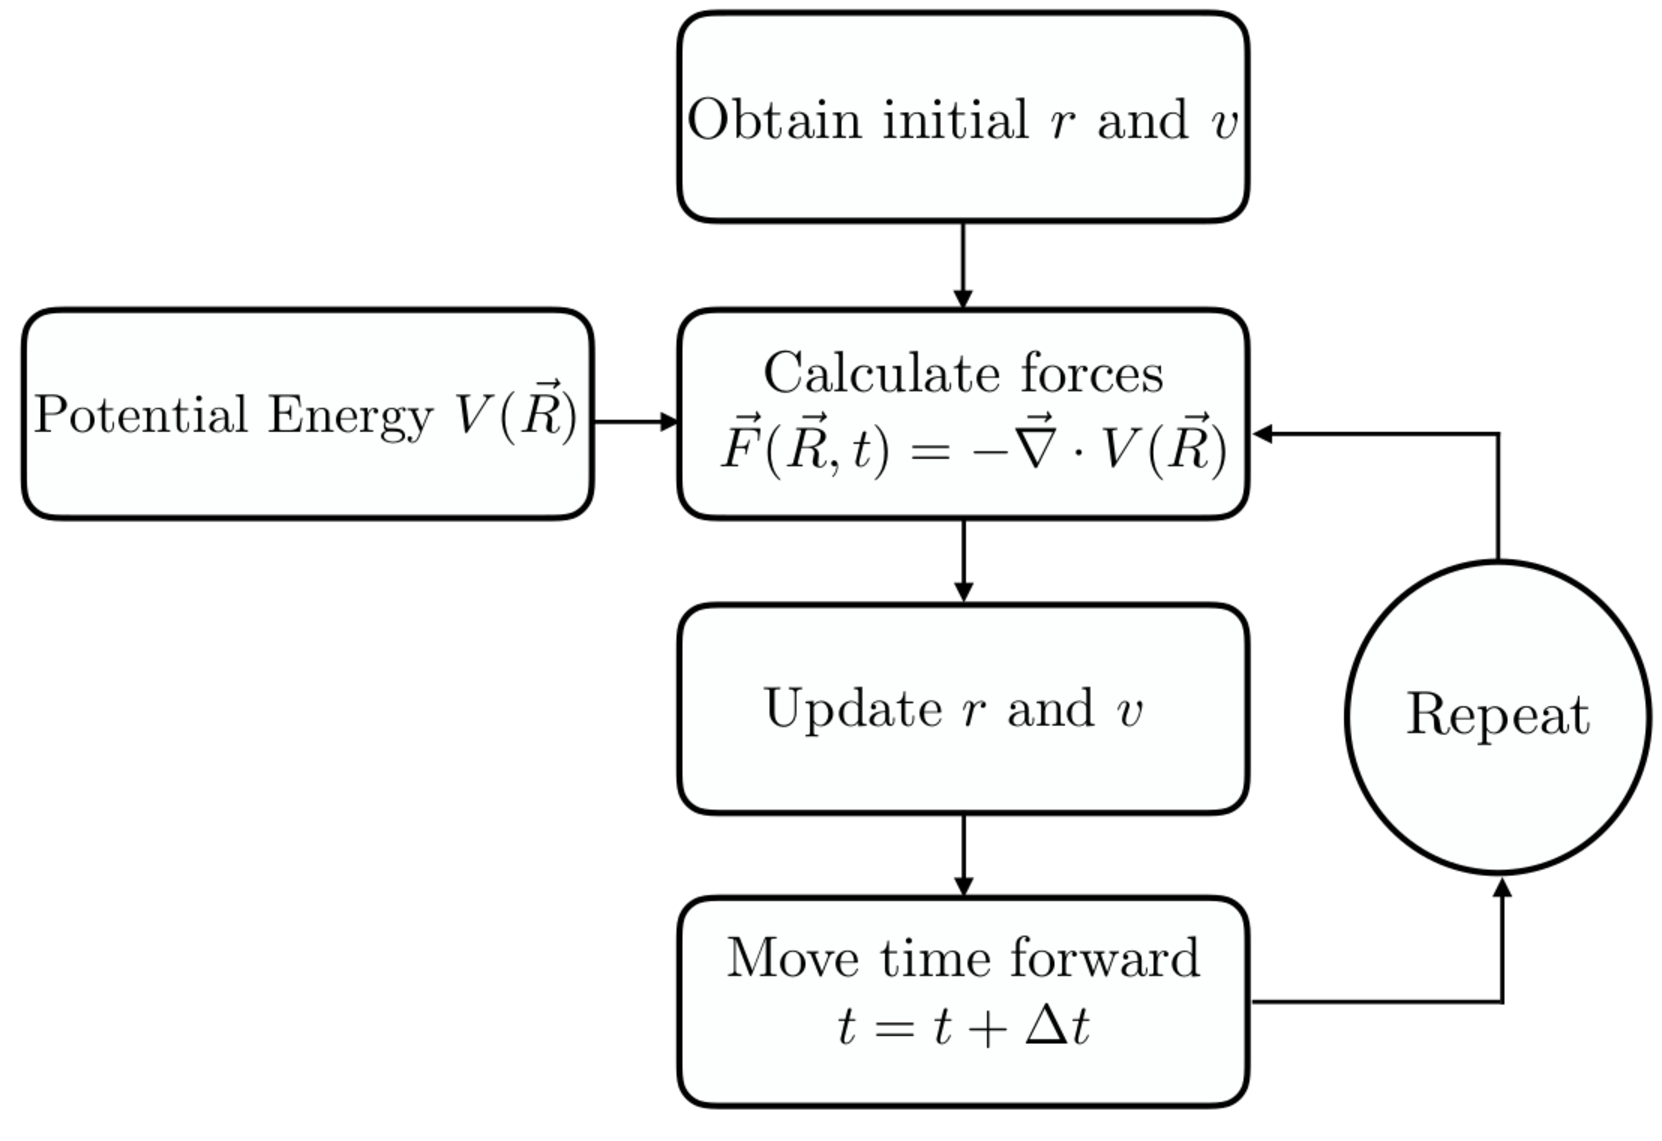
\includegraphics[scale=0.45]{figures/MDschematic.pdf}
    \caption{The initial positions, $r$, and velocities, $v$, are established in a system and from the potential energy, forces on the atoms is found. From the forces, positions can be changed then the velocities can be updated. The time can be moved forward and the process repeated at the calculated forces step until the desired time is reached.}
    \label{fig:MDschematic}
\end{figure}

Forces between each pair of atomic sites are computed from an interaction potential, where the forces are the gradient of the scalar potential:
\begin{equation}
\vec{F}(\vec{R},t) = -\vec{\nabla} \cdot V(\vec{R})
\end{equation}
These potentials are approximated using intra and inter molecular forces in the system to make an approximate potential energy surface with respect to the nuclear coordinates of the system.~\cite{Leach2001} 
\begin{equation}
   V(\vec{R}) = V_{bonded} + V_{electrostatic} + V_{vdW} + V_{metallic} +V_{constraints} + V_{hb}     
\end{equation}
The simplest of these to start with is the intra-molecular forces $V_{bonded}$, composed of bonds, bends, and torsions. Typical bonding potentials take the form of either harmonic bonds,
\begin{equation}
    V_{bond}(r) = \frac{k_{ij}}{2} (r - r_{ij}^0)^2
\end{equation}
or Morse bonds,
\begin{equation}
    V_{bond}(r) = D_{ij} [1 - \exp^{-\beta (r - r_{ij}^0)}]^2 .
\end{equation}
While other potential forms such as cubic and quartic can be used, the main form used in the following work will follow the harmonic form. In the harmonic form there are two variables that need to be provided: $k_{ij}$ and $r_{ij}^0$. The former is the spring constant associated with how the bond behaves when stretched and contracted. The latter is the equilibrium bond distance between the two atoms.

Similar to the bonding potentials, the bending potentials may take many forms. In this work, the harmonic potential,
\begin{equation}
    V_{bend} (\theta) = \frac{k_{ijk}}{2} (\theta - \theta_{ijk}^0)^2,
\end{equation}
was used, where $\theta$ is the angle between three connecting beads i, j, and k. $\theta_{ijk}^0$ is the equilibrium bend angle and $k_{ijk}$ is the spring constant for the bend.

The potential due to torsions within a bonded system is from the rotation of the plane made from the $i$, $j$, and $k$ points relative to the $l$ point:
\begin{equation}
    V_{torsions} (\phi_{ijkl})= c_1 [1 + \cos{\phi_{ijkl}}] + c_2 [1 + \cos{2\phi_{ijkl}}] + c_3 [1 + \cos{3\phi_{ijkl}}]  
\end{equation}
where the angle $\phi_{ijkl}$ is $(\hat{r}_{ij} \times \hat{r}_{jk}) \cdot (\hat{r}_{jk} \times \hat{r}_{kl})$ and $\hat{r}_{ab}$ is the unit vector between $a$ and $b$.


Inter-molecular,  or non-bonded interactions, are interactions between molecules which include the electrostatic interactions and van der Waals interactions, as well as metalic interactions.
The potential for electrostatic interactions
\begin{equation}
    V_{electrostatic} = \frac{q_i q_j}{4 \pi \epsilon_0 \mid r_{ij}\mid},
\end{equation}
describes the potential between two charged sites interacting via Coulomb's law.
Van der Waals interactions in this work are described via the Lennard Jones potential,
\begin{equation}
    V_{vdW} = 4\epsilon\bigg[\bigg(\frac{\sigma}{\mid r\mid}\bigg)^{12} + \bigg(\frac{\sigma}{\mid r\mid}\bigg)^6\big]
\end{equation}
where $\epsilon$ is the well depth when the distance between the two bodies is at the minimum and $\sigma$ is the distance the well starts from zero. 
The $\frac{1}{r^6}$ term is similar to dispersion and the $\frac{1}{r^{12}}$ term is empirically added to approximate repulsion due to electron exchange correltation.

The last, and one of the most important terms for the work is $V_{metallic}$. Quantum Sutton-Chen(qSC) potential is the metallic potential used in all the following projects.\cite{Qi:1999ph} The potential is broken into two parts: a pair potential and the local density accounting for cohension.
\begin{equation}
    V_{metallic} = \sum_i \epsilon \Bigg[ \sum_{j\neqi} V_{ij}^{pair} (r_ij) - c\sqrt{\rho_i}\Bigg]
\end{equation}
\begin{equation}    
    V_{ij}^{pair} (r) = \bigg(\frac{a_{ij}}{r_{ij}}\bigg)^{n_{ij}}
\end{equation}
\begin{equation}
    \rho_i = \sum_{i\neq j}\bigg( \frac{a_{ij}}{r_{ij}}\bigg)^{m_{ij}}
\end{equation}
For gold, which is the only metal present in this work the following values are used: $n=11$, $m=8$, $\epsilon=7.8052 x 10^-3$ eV, $c=53.582$, and $a=4.0651$ \AA.
The $epsilon$ value is the well depth of the metallic interact and $a$ is the lattice parameter of the metal. 
The qSC potential is the quantum corrected form of the Sutton-Chen potential.
Other common potential for metal interactions are Lennard-Jones and Embedded Atom Method (EAM).\cite{EAM:1986}

The last two terms in the full potential equation, $V_{constraints}$ and $V_{hb}$, hydrogen bonding, are not relevant to the simulations presented in this work.

\subsection{Representations of Atoms}
Molecular dyanamics is a lower accuracy method than first principals methods. There are different levels of simplification of the treatment of molecules.~\cite{Leach2001} 
Chiefly, there are three ways of treating the molecules in a given system that will be discussed here. 
The first, all-atom, is representing each atom within the system as a bead. In a molecule, these beads share bonds with atoms they are covalently bonded with and experiences bends and torsions within the larger molecule.

The next is a simplified version of the all-atom representation, united-atom, which compresses the hydrogen atoms onto the larger atom to which they were bonded. The mass and atomic radius of this bead is increased according to the number for hydrogens added.

United-atom calculations are faster due to the decrease in N, the number of atoms. They also are a better representation of heat transport. The vibrations of the molecules are of paramount importance in thermal transport and bonds to hydrogen have a high vibrational frequency. In molecular dynamics, the vibrational modes are occupied equally due to equipartition of the energy, thus the vibrational spectrum of the molecule will have high frequency \ce{C-H}, \ce{N-H}, or \ce{O-H} peaks. These high frequencies are irrelevant in most thermal transport calculations and thus all-atom simulations add expense and information that detracts from the low frequency picture of the system.

The last treatment discussed here is coarse-grained systems. These systems are further simplifications of the atoms present in the molecules. In coarse-grain systems, beads from the united atom model would be grouped into a single bead that represents a small molecule. The granularity of the beads can be adjusted from system to system and depends on the property desired and the timescale of the simulation. In general, coarse-graining is used widely for biologically relevant systems (i.e. proteins, lipids, etc.).
    
\subsection{Boundary Conditions}
In many simulations the desired quantity is a bulk property. To simulate a full bulk system would require too many atoms and too much time than possible within the lifetime of a graduate student. Further, the large box would have effects from the edges of the box. So how can the surface effects be avoided and simulate a bulk-like simulation?

\begin{figure}
    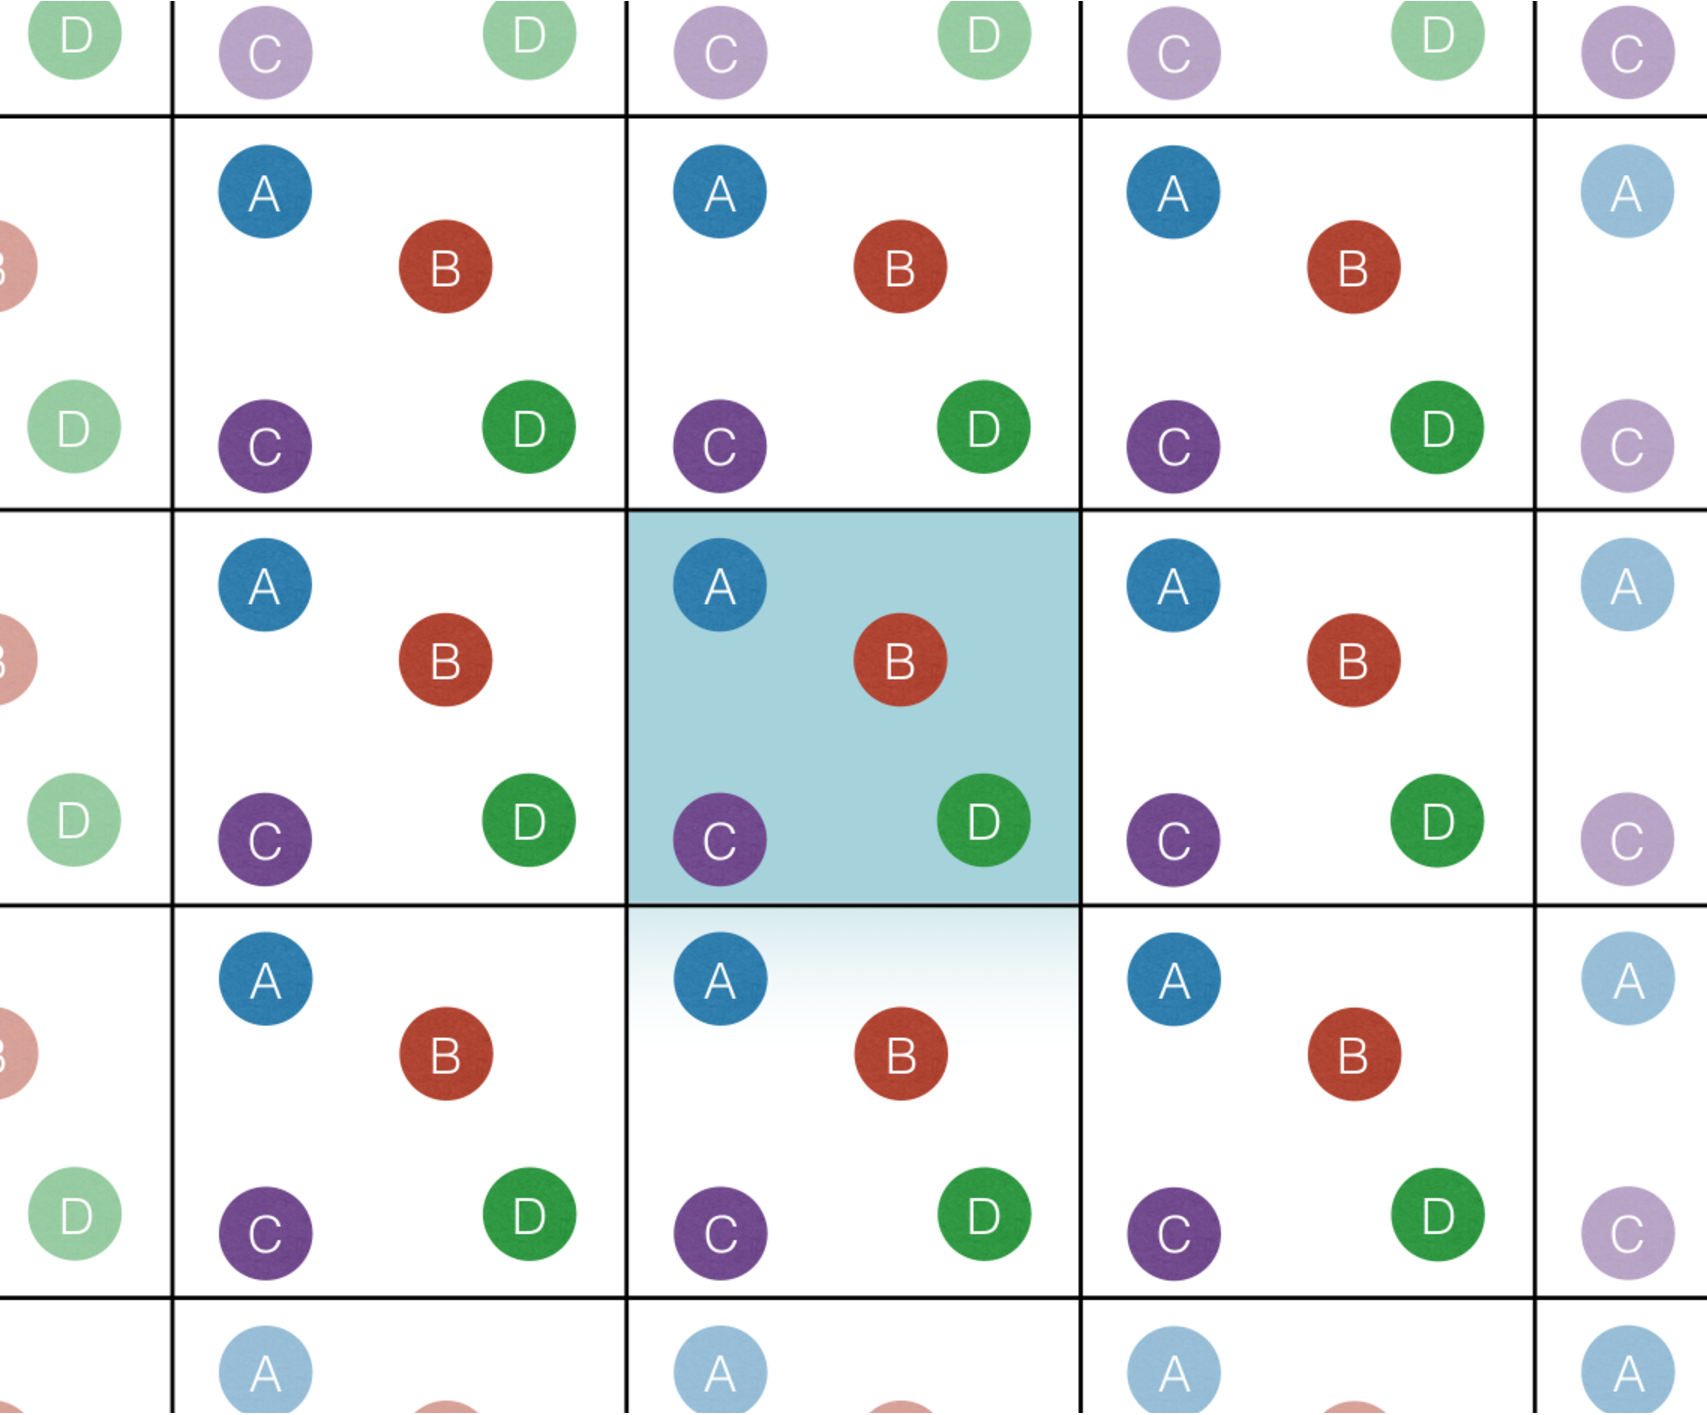
\includegraphics[scale=0.5]{figures/pbc-center.pdf}
    \caption{This figure is an example of periodic boundaries in two dimensions. Here the middle cell (colored square) is the system and each surrounding cell is an `image' of the original. As can be seen in the relation between particle A and C, sometimes the image particle provides the closest interaction or minimum image and would be within the cutoff radius when calculating interactions.}
    \label{fig:pbc}
\end{figure}

The above issues can be addressed with periodic boundary conditions. A simulation cell that has bulk-like density can reproduce bulk properties. Periodic boundary conditions are typically applied to orthorhombic simulation boxes, though any space filling geometry works. An `image' copy of the the simulation box is replicated in every direction. For example, in two dimensions periodic boundaries are represented in Figure \ref{fig:pbc}, where the simulation box has eight copies. In three dimensions, twenty-six images of the original box surround the simulation cell, for an orthorhombic box.
    
In a simulation, it is only necessary to track the particles in the central box.
The particles' images in neighboring cells are located at integer increments of the box dimension along each principal axis. 
So if the particle exits the right boundary of the cell, it will return in the box on the left boundary (from the neighboring simulation cell), which preserves the number density of the cell. 
In addition to periodic boundaries, the minimum image convention is used to make the simulation computationally tractable. A particle only interacts with the closest periodic image of another particle in the system. 
This convention requires a spherical cutoff, where a particle's non-bonded interactions with other particles end at a finite distance, $r$, from the particle which is less than half the length of the periodic box. This ensures that the particle sees one image of each particle and does not interacting with an image of itself. 

Though periodic boundaries allows for bulk properties to be found, it creates artificial periodicity in the system and might require an unreasonable system size due to the box structure. Later in this work, simulations of isolated particles are utilized to get single particle properties. 
These isolated systems use the Langevin Hull method. While there are several non-periodic methods that allow for a constant pressure, the Langevin Hull can handle heterogeneous mixtures of materials with different compressibilites.~\cite{Vardeman2011} This method is a modified version of Kohanoff, Caro, and Finnis' method for constant pressure and temperature non-periodic simulations based on Langevin dynamics.~\cite{Kohanoff:2005qm, Baltazar:2006ru} 

\begin{figure}
    \centering
    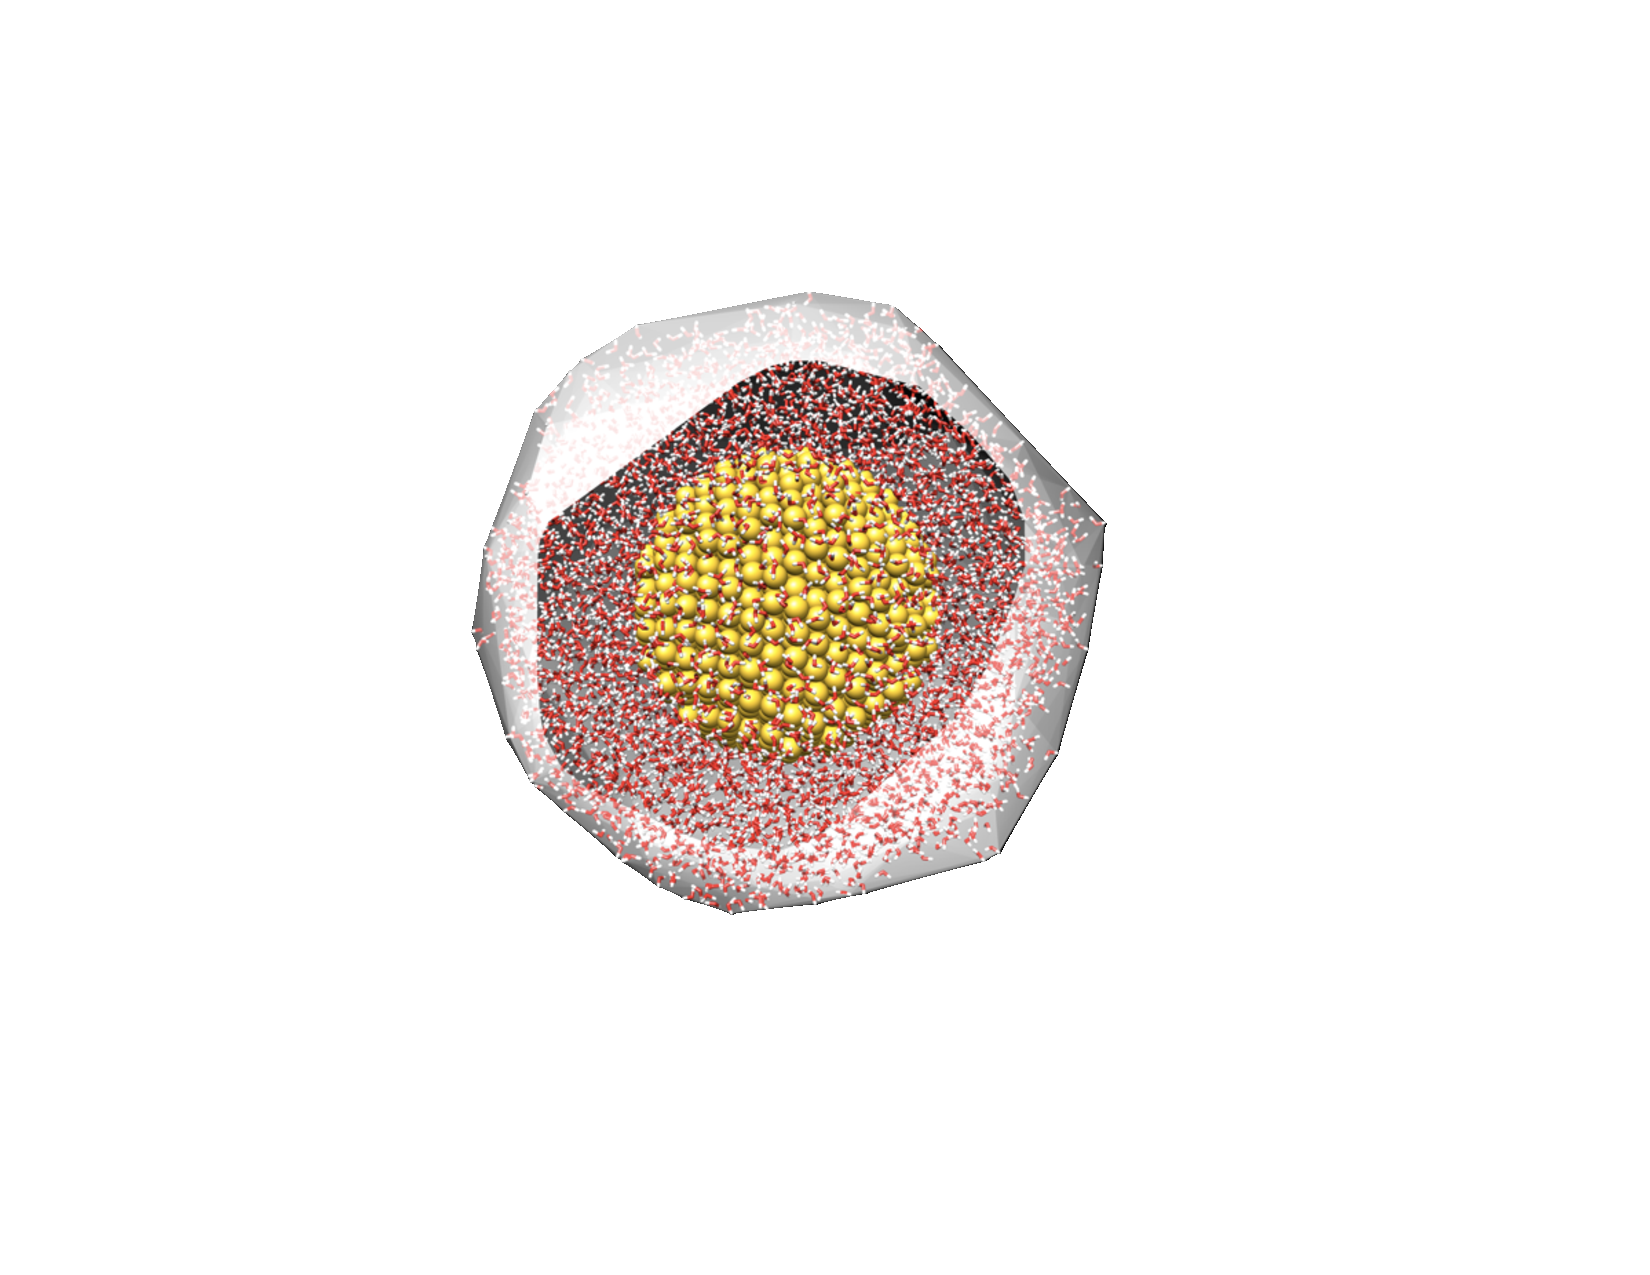
\includegraphics[scale=1]{figures/hull.pdf}
    \caption{Visualization of a gold particle solvated in water within the Langevin Hull taken from Vardeman \textit{et. al.}.~\cite{Vardeman2011}. The temperature and pressure bath interact with only the outer most atoms on the hull, the grey translucent surface. At each time step the hull is computed to ensure the atoms are interacting in the correct classifications, as edge atoms or as interior atoms.}
    \label{fig:hull}
\end{figure}

In the Langevin Hull method, the boundary of the system is a completely convex hull made of facets from points triangulated with the outermost atoms of the system. This hull interacts with a system bath that applies constant pressure and provides a thermal bath for the system through the facets of the hull. When looking at thermal properties of a system, the thermal coupling can be turned off to prevent artificial behavior due to the bath.

\section{Transport Coefficients}
Transport phenomena are controlled by the constitutive equations that describe how a material responds to various stimuli via transport.
The processes that are at the center of transport phenomena concern the transfer of mass, heat, or momentum. The transport of any of those listed would create a measurable flux in the system. The conservation equations conserve the desired property of interest in the presence of a flux.
The constitutive equations relate a transport property (diffusion, thermal conductivity, viscosity) to a flux via an empirical relationship. The flux, in all these cases, is proportional to the gradient and a constant of proportionality.

\begin{table}[h]
\centering
\caption{Constitutive and balance equations related to the transport coefficients of diffusivity, $D$, thermal conductivity, $\lambda$, and shear viscosity, $\eta$.  
\label{tab:coeff}}
\renewcommand*{\arraystretch}{2}
\begin{tabular}{ ccc }
\toprule
Transport & Constitutive & Balance\\
coefficients& equations& equations\\
\hline
$D$ & $\vec{j} = -D \cdot \vec{\nabla}c(\vec{r},t)$ & $\frac{\partial c(\vec{r},t)}{\partial t}+\vec{\nabla}\vec{j}=0$ \\
$\lambda$ & $\vec{q} = -\lambda \cdot \vec{\nabla}T(\vec{r},t)$ & $C_p \frac{\partial T(\vec{r},t)}{\partial t}+\vec{\nabla}\vec{q}=0$ \\
$\eta$ & $\sigma_{x,z} = -\eta \cdot \vec{\nabla_{z}}(\rho v_x)$ & $\rho \frac{D\vec{v}(\vec{r}, t)}{Dt}+\vec{\nabla} \overset{\leftrightarrow}{\sigma}=0$\\
\bottomrule
\end{tabular}
\end{table}
\begin{itemize}
    \item Diffusion (Fick’s Law):
$\vec{j} = -D \cdot \vec{\nabla}c(\vec{r},t)$

The diffusivity, $D$, or the diffusion coefficient is the proportionality between the concentration gradient of a species and the mass flux, $j$. 

\item Thermal Conductivity (Fourier’s Law):
$\vec{q} = -\lambda \cdot \vec{\nabla}T(\vec{r},t)$

The local heat flux density, $q$, is the produc of the conductivity of the material, $\lambda$, and the temperature gradient through the material. Therefore, $\lambda$ indicates the material's ability to conduct heat due to a temperature gradient. 

\item Viscosity (Newton’s Law of Viscosity): 
$\sigma_{x,z} = -\eta \cdot \vec{\nabla_{z}}(\rho v_x)$

The shear stress in the fluid, $\sigma$, is the product of the shear viscosity, $\eta$, and the perpendicular velocity gradient, $\vec{\nabla_{z}}(\rho v_x)$.

%\item Electrical Conductivity (Ohm's Law):
%$J = \sigma E$

%Where J, the current density at a point is equal to the electric field, E, at the same point by the material's electrical conductivity, $\sigma$.
\end{itemize}

All the transport coefficients ($D$, $\lambda$, $\eta$) describe how an instantaneous flux in a system relates to a corresponding gradient. Table \ref{tab:coeff} lists how the transport coefficients are involved in constitutive equations, where $\rho$ is the density and $C$ is the heat capacity of a material.

Transport phenomena are utilized in many fields, such as chemistry, physics, chemical engineering, electrical engineering, and mechanical engineering; to obtain the transport coefficients that describe a mechanical or chemical system. Atomistic simulations can provide insight for tuning experimental design. The three main ways to calculate transport coefficients, with a focus on thermal conductivity, will be discussed in detail in the following sections.

\subsection{Equilibruim Molecular Dynamics}
Transport properties from classical molecular dynamics simulations can be found using many methods. Equilibrium Molecular Dynamics (EMD) simulations use the most straightforward method. Under linear response theory, the transport coefficient can often be found using a relevant time correlation function to the transport coefficient of interest.~\cite{Heyes:1988ee,MASSOBRIO:1984bl,Helfand:1960os,Viscardy:2007rp,che:6888,kinaci:014106} In most cases either the Einstein relation or the Green-Kubo formulation are utilized to compute transport properties from the time correlation function in EMD.

The Einstein relation for thermal conductivity uses the Helfand moment, $G^\lambda (t)$, which is a centroid of the particle energies:
\begin{equation}
    G^\lambda (t) = \sum^{N}_{a=1} r_a (E_a - <E_a>)
\end{equation}
where $E_a$ is the energy of the particle $a$. Energy is given by the following: 
\begin{equation}
    E_a = \frac{p_a^2}{2m} + \frac{1}{2}\sum_{b\neq a} U(r_{ab})
\end{equation}
where $p_a$ is the momentum of $a$, $m$ is the mass, and $U(r_{ab})$ is the potential energy due to the presence of $a$.

The Einstein relation can  find the thermal conductivity using the fluctuations in the Helfand moment:
\begin{equation}
    \lambda = \lim_{N,V,t \rightarrow \infty} \frac{1}{2k_B T^2 Vt} \bigg< \Big[ G^\lambda (t) - G^\lambda (0) \Big]^2\bigg>
\end{equation}
where $k_B$ is the Boltzmann constant, $T$ is the temperature, $V$ is the volume, and $t$ is the time.

The equivalent Green-Kubo relation for thermal conductance is
\begin{equation}
    \lambda = \frac{1}{3Vk_BT^2}\int^\infty_0 dt <q(t) \cdot q(0)>
\end{equation}
where $q$ is the heat current.
The heat current can be found through
\begin{equation}
    q(t) = \sum^N_{i=1} E_i \vec{v_i} + \frac{1}{2}\sum_{j \neq i} \vec{r_{ij}} (f_{ij} \cdot \vec{v_j}).
\end{equation}
The first term is a summation of the energy times the velocity of all particles. The second term contains the force on atom $i$ due to atom $j$, $f_{ij}$.
In contrast to the Einstein relation where the mass, velocity, and potential are easily obtained from an equilibrium simulation, the heat current requires significantly more effort.

Both the Einstein and Green-Kubo relations for thermal conductiviy rely on correlation functions, where the long-time tails are able to significantly contribute to the integrated area and need long simulation times to achieve convergence.
The noise and poor convergence in the long-time tails give a poor estimation for the thermal conductivity and thus EMD simulations are not the best method for calculating this transport coefficient.
Moreover, these calculations have further complications when the systems contain an interface or are non-homogeneous.

\subsection{Non-Equilibruim Molecular Dynamics}
Since EMD has limitations due to the noise in the correlation function, methods in non-equilibrium molecular dynamics, NEMD, were developed that introduce a gradient into the simulations.~\cite{Backer:2005sf,Hess:2002nr,Picalek:2009rz, Vasquez:2004ty}
Typically these methods are used to impose a temperature or velocity gradient on a system to measure the corresponding transport coefficient. ~\cite{Evans:1982oq, Erpenbeck:1984qe, Evans:1986nx, Vogelsang:1988qv, Maginn:1993kl, Hess:2002nr, Schelling:2002dp, Berthier:2002ai, Evans:2002tg, Vasquez:2004ty, Backer:2005sf, Jiang:2008hc, Picalek:2009rz}
With linear response of a flux due to the applied gradient, the transport coefficient can be calculated using the constitutive equation: $J_z = -\lambda \frac{\partial T}{\partial z}$, where $\frac{\partial T}{\partial z}$ is imposed and $J_z$ is the resulting flux.
In NEMD, the temperature gradient is imposed by choosing sections of the simulation box to have particular temperatures. For example, a center portion of the system will be set to high temperature and the edges set to a lower temperature to impose the gradient. 
The imposed thermal gradient must be relatively small to maintain a linear relationship between the flux and the gradient. 
The corresponding transport coefficient, thermal conductivity, can be found if linear response holds.

Accurately measuring the thermal flux from the imposed gradient is difficult.
This method requires thermostats to maintain the thermal gradient which means that it does not ensure momentum or energy conservation and that simulations are restricted to the canonical ensemble.
Additionally, in heterogeneous systems, particularly with interfaces, it can be difficult to know what the shape of the imposed gradient should be at the boundaries of materials.

\subsection{Reverse Non-Equilibruim Molecular Dynamics}
Reverse non-equilibrium molecular dynamics (RNEMD) methods impose an unphysical flux and measure the gradient that develops.~\cite{Muller-Plathe:1997wq,Muller-Plathe:1999ao,Kuang:2012fe}
Imposed flux methods are preferable because the simulation imposes the difficult to measure quantity, the flux, causing the system to develop a gradient, which is easier to measure, between the regions where the flux is imposed. 
Since the measurement of a gradient is less complex, the imposed flux methods will typically take less time to obtain converged results, therefore the simulations are less time intensive and less costly.

The original RNEMD formulation imposes an artificial momentum flux between parallel slabs of material separated in the simulation cell. The flux was created by periodically swapping the momentum between molecules in each of the slabs in a homogeneous system.~\cite{Muller-Plathe:1997wq} 
This method was modified to obtain other transport coefficients ~\cite{Muller-Plathe:1999ao} and to handle heterogeneous systems.~\cite{Muller-plathe:2005} 
An attractive feature of RNEMD is that the algorithm conserves total linear momentum and total energy.
However, issues with large fluxes can result in non-linear gradients, where linear response can not be used to find the transport coefficient.~\cite{Tenney:2010rp}

This method has become widely used for thermal and mechanical properties of homogeneous and heterogeneous systems of solids and liquids~\cite{Muller-Plathe:1997wq,Muller-Plathe:1999ao, Tenney:2010rp}, as well as, interfaces.~\cite{Patel:2005zm, Shenogina:2009ix,Kuang:2011ef, Stocker:2013cl}
Gradients near interfaces exhibit distinct behavior at the boundaries of dissimilar materials.

Recent advances in RNEMD methodology have involved scaling particle velocities instead of swapping. The scaling method uses constraint equations that require the simulation to conserve total energy and total linear momentum.~\cite{Kuang:2011ef, Kuang:2012fe}
In addition, this RNEMD method has been extended to handle non-periodic heterogeneous systems.~\cite{Stocker:2014qq}

\section{Systems of Interest}
The systems that are explored in this work contain a solvated gold substrate or particle with heat transport from the gold to the solvent. 
Thermal properties of gold particles have been of great experimental interest, with a particular interest in detangling the important factors for transport: particle size,~\cite{Zanjani2014,Liu2015,Wilhelmsen2015,Stocker2016,Tascini2016} composition,~\cite{Wilson:2002uq, Ong:2013rt} surface modification,~\cite{kuang:AuThl,Ong:2013rt,Ong:2014yq,Liu2015,Stocker2016,Hannah2015,Park2016,Leitner2017} surface supports,~\cite{Park2012} exposed surface facets,~\cite{Hannah2015} and the chemical details of the environment.~\cite{Ge2006,Park2012,Ong:2013rt,Ong:2014yq,Wilhelmsen2015,Park2016} 

Three distinct studies examining interfacial thermal conductivity and heat transport will be explored with three different systems in this work.
The first system contains nanospheres with a range of particle radii and ligands with different length and rigidity.~\cite{Stocker2016}
The second system strips away the ligand layer and looks at bare particles with the intention of finding the role of in particle morphology.~\cite{Neidhart}
How exactly does the surface of the particle affect heat transport?
The third system looks at a more complex problem: how does the particle size and the system solvent change thermal conductivity of a nanoarray?
To simplify the atomistic models, we use a united-atom model for the ligand layer and solvent.
All the non-periodic systems use the Langevin Hull~\cite{Vardeman2011} and RNEMD methods for calculating transport properties.~\cite{Stocker:2014qq}


%%%%%%%%%%%%%%%%%%%%%%%%%%%%%%%%%%%%%%%%%%%%%%%%%%%%%%%%%%%%%%%%%%%%%%%%%%%%%%%%%%%
%		CHAPTER 2 -- Ligand Dependence of the Thermal Conductivity
%%%%%%%%%%%%%%%%%%%%%%%%%%%%%%%%%%%%%%%%%%%%%%%%%%%%%%%%%%%%%%%%%%%%%%%%%%%%%%%%%%%

\chapter{INTERFACIAL THERMAL CONDUCTANCE OF THIOLATE-PROTECTED GOLD NANOSPHERES}

\section{Introduction}
  Molecular dynamics simulations of thiolate-protected and solvated gold nanoparticles were carried out in the presence of a non-equilibrium heat flux between the solvent and the core of the particle. The interfacial thermal conductance ($G$) was computed for these interfaces, and the behavior of the thermal conductance was studied as a function of particle size, ligand flexibility, and ligand chain length. In all cases, thermal conductance of the ligand-protected particles was higher than the bare metal--solvent interface.  A number of mechanisms for the enhanced conductance were investigated, including thiolate-driven corrugation of the metal surface, solvent ordering at the interface, solvent-ligand interpenetration, and ligand ordering relative to the particle
  surface. Only the smallest particles exhibited significant
  corrugation.  All ligands permitted substantial solvent-ligand
  interpenetration, and ligand chain length has a significant
  influence on the orientational ordering of interfacial solvent.
  Solvent -- ligand vibrational overlap, particularly in the low
  frequency range ($< 80 \mathrm{cm}^{-1}$) was significantly altered
  by ligand rigidity, and had direct influence on the interfacial
  thermal conductance.
%\end{abstract}


Heat transport across various nanostructured interfaces has been the
subject of intense experimental
interest,\cite{Wilson:2002uq,Ge:2004yg,Shenogina:2009ix,Wang10082007,Schmidt:2008ad,Juve:2009pt,Alper:2010pd,Harikrishna:2013ys}
and the interfacial thermal conductance, $G$, is the principal
quantity of interest for understanding interfacial heat
transport.\cite{Cahill:2003fk} Because nanoparticles have a
significant fraction of their atoms at the particle / solvent
interface, the chemical details of these interfaces govern the thermal
transport properties.  Time-domain thermoreflectance (TDTR)
measurements on planar self-assembled monolayer (SAM) junctions
between quartz and gold films showed that surface chemistry,
particularly the density of covalent bonds to the gold surface, can
control energy transport between the two solids.\cite{Losego:2012fr}
Experiments and simulations on three-dimensional nanocrystal arrays
have similarly shown that surface-attached ligands mediate the thermal
transport in these materials, placing particular importance on the
overlap between the ligand and nanoparticle vibrational densities of
states.\cite{Ong:2013rt,Ong:2014yq} Likewise, simulations of
polymer-coated gold nanoparticles in water have shown that the surface
coating introduces a dominant thermal transport channel to the
surrounding solvent.\cite{Soussi:2015fj}

For ligand-protected nanoparticles in a solvent, there may be three
distinct heat transfer processes: (1) from the particles to the
ligands, (2) vibrational energy tranfer along the length of the
ligand, followed by (3) heat transport from the ligand to the
surrounding solvent.\cite{Ge:2006kx}

Heat transport at the gold-alkylthiolate-solvent interface has been
previously explored both through molecular dynamics simulations and
via
TDTR.\cite{Kikugawa:2009vn,Kuang:2011ef,Stocker:2013cl,Tian:2015uq}
Most of these studies have found that alkylthiolates enhance the
thermal conductance to the solvent, and that the vibrational overlap
provided by the chemically-bound ligand species plays a role in this
enhancement.

Reverse nonequilibrium molecular dynamics (RNEMD)
methods~\cite{Muller-Plathe:1997wq} have been previously applied to
calculate the thermal conductance at flat (111) metal / organic
solvent interfaces that had been chemically protected by varying
coverages of alkanethiolate groups.\cite{Kuang:2011ef} These
simulations suggested an explanation for the increased thermal
conductivity at alkanethiol-capped metal surfaces compared with bare
metal interfaces.  Specifically, the chemical bond between the metal
and the ligand introduces a vibrational overlap that is not present
without the protecting group, and the overlap between the vibrational
spectra (metal to ligand, ligand to solvent) provides a mechanism for
rapid thermal transport across the interface. The simulations also
suggested that this phenomenon is a non-monotonic function of the
fractional coverage of the surface, as moderate coverages allow energy
transfer to solvent molecules that come into close contact with the
ligands.

Similarly, simulations of mixed-chain alkylthiolate surfaces
showed that solvent trapped close to the interface can be efficient at
moving thermal energy away from the surface.\cite{Stocker:2013cl}
Trapped solvent molecules that were orientationally aligned with
nearby ligands were able to increase the thermal conductance of the
interface.  This indicates that the ligand-to-solvent vibrational
energy transfer is a key feature for increasing particle-to-solvent
thermal conductance.

RNEMD methods have been extended for use in non-periodic geometries
by creating scaling/shearing moves between concentric regions of a
simulation.\cite{Stocker:2014qq} In this section, a
non-periodic variant of RNEMD has been applied to investigate the role that
curved nanoparticle surfaces play in heat and mass transport.  On
planar surfaces, it has been seen that orientational ordering of surface
protecting ligands had a large effect on the heat conduction from the
metal to the solvent.\cite{Stocker:2013cl}
 Smaller nanoparticles have high surface curvature that creates gaps in well-ordered self-assembled monolayers,
and the effect of those gaps on the thermal conductance is unknown.

%%%%%%%%%%%%%%%%%%%%%%%%%%%%%%%%%%%%%%%%%%%%%%%%%%%%%%%%%%%%%%%%%%%%%%%%%%%%%%%%%%%
%		INTERFACIAL THERMAL CONDUCTANCE OF METALLIC NANOPARTICLES
%%%%%%%%%%%%%%%%%%%%%%%%%%%%%%%%%%%%%%%%%%%%%%%%%%%%%%%%%%%%%%%%%%%%%%%%%%%%%%%%%%%
\section{Interfacial Thermal Conductance of Metallic Nanoparticles}

For a solvated nanoparticle, it is possible to define a critical value
for the interfacial thermal conductance,
\begin{equation}
G_c = \frac{3 C_s \Lambda_s}{R C_p}
\end{equation}
which depends on the solvent heat capacity, $C_s$, solvent thermal
conductivity, $\Lambda_s$, particle radius, $R$, and nanoparticle heat
capacity, $C_p$.\cite{Wilson:2002uq} In the limit of infinite
interfacial thermal conductance, $G \gg G_c$, cooling of the
nanoparticle is limited by the solvent properties, $C_s$ and
$\Lambda_s$.  In the opposite limit, $G \ll G_c$, the heat dissipation
is controlled by the thermal conductance of the particle / fluid
interface. It is this regime with which this study is concerned, where
properties of ligands and the particle surface may be tuned to
manipulate the rate of cooling for solvated nanoparticles.  Based on
estimates of $G$ from previous simulations as well as experimental
results for solvated nanostructures, gold nanoparticles solvated in
hexane are in the $G \ll G_c$ regime for radii smaller than 40 nm. The
particles included in this study are more than an order of magnitude
smaller than this critical radius, therefore the heat dissipation should be
controlled entirely by the surface features of the particle / ligand /
solvent interface.

%%%%%%%%%%%%%%%%%%%%%%%%%%%%%%%%%%%%%%%%%%%%%%%%%%%%%%%%%%%%%%%%%%%%%%%%%%%%%%%%%%%
%		STRUCTURE OF SELF-ASSEMBLED MONOLAYERS ON NANOPARTICLES
%%%%%%%%%%%%%%%%%%%%%%%%%%%%%%%%%%%%%%%%%%%%%%%%%%%%%%%%%%%%%%%%%%%%%%%%%%%%%%%%%%%
\subsection{Structures of Self-Assembled Monolayers on Nanoparticles}

Though the ligand packing on planar surfaces has been characterized
for many different ligands and surface facets, it is not obvious
\emph{a priori} how the same ligands will behave on the highly curved
surfaces of spherical nanoparticles. Thus, as new applications of
ligand-stabilized nanostructures have been proposed, the structure and
dynamics of ligands on metallic nanoparticles have been studied using
molecular simulation,\cite{Henz:2008qf} NMR, XPS, FTIR,
calorimetry, and surface
microscopies.\cite{Badia1996:2,Badia1996,Badia1997:2,Badia1997,Badia2000}
Badia, \textit{et al.} used transmission electron microscopy to
determine that alkanethiol ligands on gold nanoparticles pack
approximately 30\% more densely than on planar Au(111)
surfaces.\cite{Badia1996:2} Subsequent experiments demonstrated that
even at full coverages, surface curvature creates voids between linear
ligand chains that can be filled via interdigitation of ligands on
neighboring particles.\cite{Badia1996} The molecular dynamics
simulations of Henz, \textit{et al.} indicate that at low coverages,
the thiolate alkane chains will lie flat on the nanoparticle
surface\cite{Henz:2008qf} Above 90\% coverage, the ligands
stand upright and recover the rigidity and tilt angle displayed on
planar facets. Their simulations also indicate a high degree of mixing
between the thiolate sulfur atoms and surface gold atoms at high
coverages.

In this work, thiolated gold nanospheres were modeled using a united
atom force field and non-equilibrium molecular dynamics. Gold
nanoparticles with radii ranging from 10 - 25 \AA\ were created from a
bulk fcc lattice.  These particles were passivated with a 50\%
coverage (compared with the coverage densities reported by Badia
\textit{et al.}) of a selection of thiolates.  Three straight-chain
thiolates of varying chain lengths and rigidities were utilized.
These are summarized in Fig. \ref{fig:structures}.  The passivated
particles were then solvated in hexane.  Details on the united atom
force field are given below.

\begin{figure}
  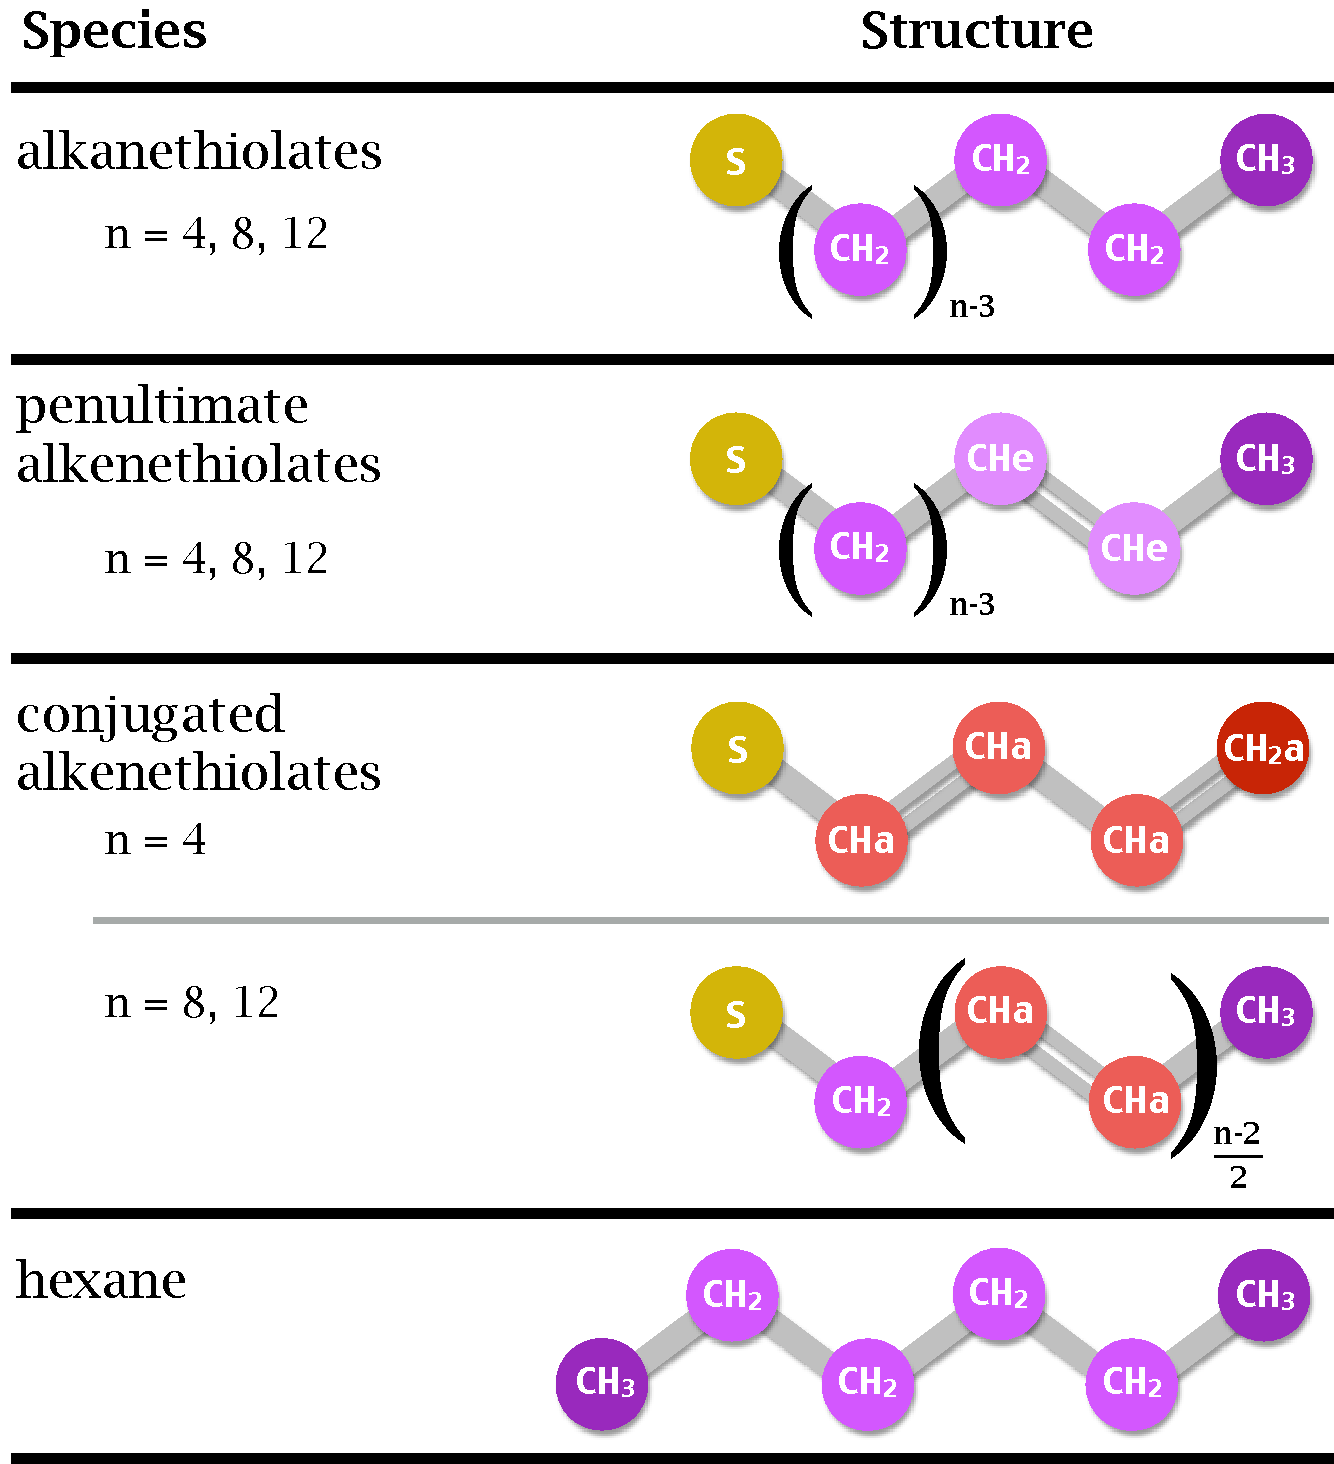
\includegraphics[width=\linewidth]{figures/structures}
  \caption{Topologies of the thiolate capping agents and solvent
    utilized in the simulations. The chemically-distinct sites (S,
    \ce{CH2}, \ce{CH3}, CHe, CHa and \ce{CH2a}) are treated as united
    atoms. Most parameters are taken from references
    \bibpunct{}{}{,}{n}{}{,} \protect\cite{TraPPE-UA.alkanes},
    \protect\cite{TraPPE-UA.alkylbenzenes}
    \protect\cite{TraPPE-UA.thiols}. Cross-interactions with the Au
    atoms were adapted from references
    \protect\cite{landman:1998},~\protect\cite{vlugt:cpc2007154},~and
    \protect\cite{hautman:4994}.}
  \label{fig:structures}
\bibpunct{[}{]}{,}{n}{}{,}
\end{figure}


%%%%%%%%%%%%%%%%%%%%%%%%%%%%%%%%%%%%%%%%%%%%%%%%%%%%%%%%%%%%%%%%%%%%%%%%%%%%%%%%%%%
%		COMPUTATIONAL DETAILS
%%%%%%%%%%%%%%%%%%%%%%%%%%%%%%%%%%%%%%%%%%%%%%%%%%%%%%%%%%%%%%%%%%%%%%%%%%%%%%%%%%%
\section{Computational Details}

%%%%%%%%%%%%%%%%%%%%%%%%%%%%%%%%%%%%%%%%%%%%%%%%%%%%%%%%%%%%%%%%%%%%%%%%%%%%%%%%%%%
%		NON-PERIODIC VSS-RNEMD METHODOLOGY
%%%%%%%%%%%%%%%%%%%%%%%%%%%%%%%%%%%%%%%%%%%%%%%%%%%%%%%%%%%%%%%%%%%%%%%%%%%%%%%%%%%
\subsection{Creating a thermal flux between particles and solvent}

The non-periodic variant of the velocity shearing and scaling RNEMD
algorithm (VSS-RNEMD)\cite{Stocker:2014qq} applies a series of
velocity scaling and shearing moves at regular intervals to impose a
flux between two concentric spherical regions. The scaling coefficients 
$a$ and $b$ are solved for to impose a thermal
flux between the shells (without an accompanying angular shear).
\begin{eqnarray}
	a = \sqrt{1 - \frac{q_r \Delta t}{K_a - K_a^\mathrm{rot}}}\\ \nonumber\\
	b = \sqrt{1 + \frac{q_r \Delta t}{K_b - K_b^\mathrm{rot}}}
\end{eqnarray}
at each time interval.  These scaling coefficients conserve total
kinetic energy and angular momentum subject to an imposed heat rate,
$q_r$.  The coefficients also depend on the instantaneous kinetic
energy, $K_{\{a,b\}}$, and the total rotational kinetic energy of each
shell, $K_{\{a,b\}}^\mathrm{rot} = \sum_i m_i \left( \mathbf{v}_i
  \times \mathbf{r}_i \right)^2 / 2$.

The scaling coefficients are determined and the velocity changes are
applied at regular intervals, 
\begin{eqnarray}
	\mathbf{v}_i \leftarrow a \left ( \mathbf{v}_i - \left < \omega_a \right > \times \mathbf{r}_i \right ) + \left < \omega_a \right > \times \mathbf{r}_i~~\:\\
	\mathbf{v}_j \leftarrow b \left ( \mathbf{v}_j - \left < \omega_b \right > \times \mathbf{r}_j \right ) + \left < \omega_b \right > \times \mathbf{r}_j.
\end{eqnarray}
Here $\left < \omega_a \right > \times \mathbf{r}_i$ is the
contribution to the velocity of particle $i$ due to the overall
angular velocity of the $a$ shell. In the absence of an angular
momentum flux, the angular velocity $\left < \omega_a \right >$ of the
shell is nearly 0 and the resultant particle velocity is a nearly
linear scaling of the initial velocity by the coefficient $a$ or $b$.

Repeated application of this thermal energy exchange yields a radial
temperature profile for the solvated nanoparticles that depends
linearly on the applied heat rate, $q_r$. Similar to the behavior in
the slab geometries, the temperature profiles have discontinuities at
the interfaces between dissimilar materials.  The size of the
discontinuity depends on the interfacial thermal conductance, which is
the primary quantity of interest.

%%%%%%%%%%%%%%%%%%%%%%%%%%%%%%%%%%%%%%%%%%%%%%%%%%%%%%%%%%%%%%%%%%%%%%%%%%%%%%%%%%%
%		CALCULATING TRANSPORT PROPERTIES
%%%%%%%%%%%%%%%%%%%%%%%%%%%%%%%%%%%%%%%%%%%%%%%%%%%%%%%%%%%%%%%%%%%%%%%%%%%%%%%%%%%
%%%%%%%%%%%%%%%%%%%%%%%%%%%%%%%%%%%%%%%%%%%%%%%%%%%%%%%%%%%%%%%%%%%%%%%%%%%%%%%%%%%
%		INTERFACIAL THERMAL CONDUCTANCE
%%%%%%%%%%%%%%%%%%%%%%%%%%%%%%%%%%%%%%%%%%%%%%%%%%%%%%%%%%%%%%%%%%%%%%%%%%%%%%%%%%%
\subsection{Interfacial Thermal Conductance}

The thermal conductance of each spherical shell may be defined as the inverse
Kapitza resistance of the shell.\cite{Stocker:2014qq}
To describe the thermal conductance
of an interface of considerable thickness -- such as the ligand layers
shown here -- sum the individual thermal resistances of each
concentric spherical shell to arrive at the inverse of the total
interfacial thermal conductance. 
In concentric spherical shells, the
intermediate temperatures and surface areas remain in the final sum,
requiring the use of a series of individual resistance terms:

\begin{equation}
  \frac{1}{G} = R_\mathrm{total} = \frac{1}{q_r} \sum_i \left(T_{i+i} -
    T_i\right) 4 \pi r_i^2.
\end{equation}

The longest ligand considered here is in excess of 15 \AA\ in length,
and 10 concentric spherical shells are used to describe the total
interfacial thermal conductance of the ligand layer.

%%%%%%%%%%%%%%%%%%%%%%%%%%%%%%%%%%%%%%%%%%%%%%%%%%%%%%%%%%%%%%%%%%%%%%%%%%%%%%%%%%%
%		FORCE FIELDS
%%%%%%%%%%%%%%%%%%%%%%%%%%%%%%%%%%%%%%%%%%%%%%%%%%%%%%%%%%%%%%%%%%%%%%%%%%%%%%%%%%%
\subsection{Force Fields}

Throughout this work, gold -- gold interactions are described by the
quantum Sutton-Chen (QSC) model.\cite{Qi:1999ph} Previous
work\cite{Kuang:2011ef} has demonstrated that the electronic
contributions to heat conduction (which are missing from the QSC
model) across heterogeneous metal / non-metal interfaces are
negligible compared to phonon excitation, which is captured by the
classical model. The hexane solvent is described by the TraPPE united
atom model,\cite{TraPPE-UA.alkanes} where sites are located at the
carbon centers for alkyl groups. The TraPPE-UA model for hexane
provides both computational efficiency and reasonable accuracy for
bulk thermal conductivity values. Bonding interactions were used for
intra-molecular sites closer than 3 bonds. Effective Lennard-Jones
potentials were used for non-bonded interactions.

\begin{table}[h]
\bibpunct{}{}{,}{n}{}{,}
\centering
\caption{Non-bonded interaction parameters (including cross interactions with Au atoms). \label{tab:atypes}}
\begin{tabular}{ c|cccccl }
 \toprule
Site & mass & $\sigma_{ii}$ & $\epsilon_{ii}$ & $\sigma_{\ce{Au}-i}$ & $\epsilon_{\ce{Au}-i}$  & source \\
     & (amu)& (\AA)        & (kcal/mol)     & (\AA)             &  (kcal/mol)          &  \\
 \colrule
 \ce{CH3}    & 15.04    & 3.75  & 0.1947 & 3.54   & 0.2146 & Refs. \protect\cite{TraPPE-UA.alkanes}, \protect\cite{vlugt:cpc2007154} and \protect\cite{landman:1998}\\
 \ce{CH2}    & 14.03    & 3.95  & 0.09141& 3.54   & 0.1749 & Refs. \protect\cite{TraPPE-UA.alkanes}, \protect\cite{vlugt:cpc2007154} and \protect\cite{landman:1998}\\
 CHene       & 13.02    & 3.73  & 0.09340& 3.4625 & 0.1680 & Refs. \protect\cite{TraPPE-UA.alkylbenzenes}, \protect\cite{vlugt:cpc2007154} and \protect\cite{landman:1998}\\
 S           & 32.0655  & 4.45  & 0.2504 & 2.40   & 8.465  & Refs. \protect\cite{landman:1998} ($\sigma$) and \protect\cite{vlugt:cpc2007154} ($\epsilon$) \\
 CHar        & 13.02    & 3.695 & 0.1004 & 3.4625 & 0.1680 & Refs. \protect\cite{TraPPE-UA.alkylbenzenes} and \protect\cite{vlugt:cpc2007154}\\
 \ce{CH2ar}  & 14.03    & 3.695 & 0.1004 & 3.4625 & 0.1680 & Refs. \protect\cite{TraPPE-UA.alkylbenzenes} and \protect\cite{vlugt:cpc2007154}\\
 \botrule
\end{tabular}
\bibpunct{[}{]}{,}{n}{,}{,}
\end{table}


The TraPPE-UA force field includes parameters for thiol
molecules\cite{TraPPE-UA.thiols} as well as unsaturated and aromatic
carbon sites.\cite{TraPPE-UA.alkylbenzenes} These were used for the
thiolate molecules in our simulations, and missing parameters for the
ligands were supplemented using fits described below.
Bonds are rigid in TraPPE-UA, so although equilibrium
bond distances were taken from this force field, flexible bonds were
implemented using bond stretching spring constants adapted from the
OPLS-AA force field.\cite{Jorgensen:1996sf}

\begin{table}[h]
\bibpunct{}{}{,}{n}{}{,}
\centering
\caption{Bond parameters. \label{tab:bond}}
\begin{tabular}{ cc|ccl }
 \toprule
 $i$&$j$ & $r_0$ & $k_\mathrm{bond}$ & source \\
    &    & (\AA) & $(\mathrm{~kcal/mole/\AA}^2)$ & \\
 \colrule
\ce{CH3}   & \ce{CH3} & 1.540   & 536  & Refs. \protect\cite{TraPPE-UA.alkanes} and \protect\cite{Jorgensen:1996sf}\\
\ce{CH3}   & \ce{CH2} & 1.540   & 536  & Refs. \protect\cite{TraPPE-UA.alkanes} and \protect\cite{Jorgensen:1996sf} \\
\ce{CH2}   & \ce{CH2} & 1.540   & 536  & Refs. \protect\cite{TraPPE-UA.alkanes} and \protect\cite{Jorgensen:1996sf} \\
CHene      & CHene    & 1.330   & 1098 & Refs. \protect\cite{TraPPE-UA.alkylbenzenes} and \protect\cite{Jorgensen:1996sf}\\
\ce{CH3}   & CHene    & 1.540   & 634  & Refs. \protect\cite{TraPPE-UA.alkylbenzenes} and \protect\cite{Jorgensen:1996sf} \\
\ce{CH2}   & CHene    & 1.540   & 634  & Refs. \protect\cite{TraPPE-UA.alkylbenzenes} and \protect\cite{Jorgensen:1996sf} \\
S          & \ce{CH2} & 1.820   & 444  & Refs. \protect\cite{TraPPE-UA.thiols} and \protect\cite{Jorgensen:1996sf} \\
CHar       & CHar     & 1.40    & 938  & Refs. \protect\cite{TraPPE-UA.alkylbenzenes} and \protect\cite{Jorgensen:1996sf} \\
CHar       & \ce{CH2} & 1.540   & 536  & Refs. \protect\cite{TraPPE-UA.alkylbenzenes} and \protect\cite{Jorgensen:1996sf}\\
CHar       & \ce{CH3} & 1.540   & 536  & Refs. \protect\cite{TraPPE-UA.alkylbenzenes} and \protect\cite{Jorgensen:1996sf}\\
\ce{CH2ar} & CHar     & 1.40    & 938  & Refs. \protect\cite{TraPPE-UA.alkylbenzenes} and \protect\cite{Jorgensen:1996sf} \\
S          & CHar     & 1.80384 & 527.951 & This Work \\
 \botrule
\end{tabular}
\bibpunct{[}{]}{,}{n}{,}{,}
\end{table}

Parameters not found in the TraPPE-UA force field for the
intramolecular interactions of the conjugated and the penultimate
alkenethiolate ligands were calculated using constrained geometry
scans using the B3LYP functional~\cite{Becke:1993kq,Lee:1988qf} and
the 6-31G(d,p) basis set. Structures were scanned starting at the
minimum energy gas phase structure for small ($C_4$) ligands.  Only
one degree of freedom was constrained for any given scan -- all other
atoms were allowed to minimize subject to that constraint.  The
resulting potential energy surfaces were fit to a harmonic potential
for the bond stretching,
\begin{equation}
V_\mathrm{bond} = \frac{k_\mathrm{bond}}{2} \left( r - r_0 \right)^2,
\end{equation}
and angle bending potentials,
\begin{equation}
V_\mathrm{bend} = \frac{k_\mathrm{bend}}{2} \left(\theta - \theta_0\right)^2.
\end{equation}
Torsional potentials were fit to the TraPPE torsional function,
\begin{equation}
V_\mathrm{tor} = c_0 + c_1  \left(1 + \cos\phi \right) + c_2  \left(1 - \cos 2\phi \right) + c_3  \left(1 + \cos 3 \phi \right).
\end{equation}

For the penultimate thiolate ligands, the model molecule used was
2-Butene-1-thiol, for which one bend angle (\ce{S-CH2-CHene}) was
scanned to fit an equilibrium angle and force constant, as well as one
torsion (\ce{S-CH2-CHene-CHene}).  The parameters for these two
potentials also served as model for the longer conjugated thiolate
ligands which require bend angle parameters for (\ce{S-CH2-CHar}) and
torsion parameters for (\ce{S-CH2-CHar-CHar}).

For the $C_4$ conjugated thiolate ligands, the model molecule for the
quantum mechanical calculations was 1,3-Butadiene-1-thiol.  This
ligand required fitting one bond (\ce{S-CHar}), and one bend angle
(\ce{S-CHar-CHar}).

The geometries of the model molecules were optimized prior to
performing the constrained angle scans, and the fit values for the
bond, bend, and torsional parameters were in relatively good agreement
with similar parameters already present in TraPPE.

\begin{table}[h]
\bibpunct{}{}{,}{n}{,}{,}
\centering
\caption{Bend angle parameters. The central atom in the bend is atom $j$.\label{tab:bend}}
\begin{tabular}{ ccc|ccl }
\toprule
 $i$&$j$&$k$ & $\theta_0$ & $k_\mathrm{bend}$ & source\\
    &   &    & ($\degree$) & (kcal/mol/rad\textsuperscript{2}) & \\
 \colrule
\ce{CH2} & \ce{CH2} & S         & 114.0   &   124.20& Ref. \protect\cite{TraPPE-UA.thiols}\\
\ce{CH3} & \ce{CH2} & \ce{CH2}  & 114.0   &   124.20& Ref. \protect\cite{TraPPE-UA.thiols}\\
\ce{CH2} & \ce{CH2} & \ce{CH2}  & 114.0   &   124.20& Ref. \protect\cite{TraPPE-UA.thiols}\\
CHene    & CHene    & \ce{CH3}  & 119.7   &   139.94& Ref. \protect\cite{TraPPE-UA.alkylbenzenes}\\
CHene    & CHene    & \ce{CH2}  & 119.7   &   139.94& Ref. \protect\cite{TraPPE-UA.alkylbenzenes}\\
\ce{CH2} & \ce{CH2} & CHene     & 114.0   &   124.20& Ref. \protect\cite{TraPPE-UA.alkylbenzenes}\\
CHar     & CHar     & CHar      & 120.0   &   126.0 & Refs. \protect\cite{TraPPE-UA.alkylbenzenes} and \protect\cite{Jorgensen:1996sf}\\
CHar     & CHar     & \ce{CH2}  & 120.0   &   140.0 & Refs. \protect\cite{TraPPE-UA.alkylbenzenes} and \protect\cite{Jorgensen:1996sf}\\
CHar     & CHar     & \ce{CH3}  & 120.0   &   140.0 & Refs. \protect\cite{TraPPE-UA.alkylbenzenes} and \protect\cite{Jorgensen:1996sf}\\
CHar     & CHar     & \ce{CH2ar}& 120.0   &   126.0 & Refs. \protect\cite{TraPPE-UA.alkylbenzenes} and \protect\cite{Jorgensen:1996sf}\\
S        & \ce{CH2} & CHene     & 109.97  &  127.37 & This work  \\
S        & \ce{CH2} & CHar      & 109.97  &  127.37 & This work  \\
S        & CHar     & CHar      & 123.911 & 138.093 & This work  \\
 \botrule
\end{tabular}
\bibpunct{[}{]}{,}{n}{,}{,}
\end{table}

\begin{table}[h]
\bibpunct{}{}{,}{n}{,}{,}
\centering
\caption{Torsion parameters. The central atoms for each torsion are atoms $j$ and $k$,
  and wildcard atom types are denoted by ``X''.  All $c_n$ parameters
  have units of kcal/mol. The torsions around carbon-carbon double bonds
  are harmonic and assume a trans (180$\degree$) geometry.  The force
  constant for this torsion is given in $\mathrm{kcal~mol~}^{-1}\mathrm{degrees}^{-2}$.  \label{tab:torsion}}
\begin{tabular}{ cccc|ccccl }
\toprule
 $i$&$j$&$k$&$l$& $c_0$&$c_1$& $c_2$ & $c_3$ & source\\
 \colrule
\ce{CH3} & \ce{CH2} & \ce{CH2} & \ce{CH2} & 0.0     & 0.7055   & -0.13551 &  1.5725    & Ref. \protect\cite{TraPPE-UA.alkanes}\\
\ce{CH2} & \ce{CH2} & \ce{CH2} & \ce{CH2} & 0.0     & 0.7055   & -0.13551 &  1.5725    & Ref. \protect\cite{TraPPE-UA.alkanes}\\
\ce{CH2} & \ce{CH2} & \ce{CH2} & S        & 0.0     & 0.7055   & -0.13551 &  1.5725    & Ref. \protect\cite{TraPPE-UA.thiols}\\ \colrule
X        & CHene    & CHene    & X        & \multicolumn{4}{c}{\multirow{2}{*}{$V = \frac{0.008112}{2} (\phi - 180.0)^2$}} & \multirow{2}{*}{Ref. \protect\cite{TraPPE-UA.alkylbenzenes}} \\
X        & CHar     & CHar     & X        &         & & & & \\ \colrule
\ce{CH2} & \ce{CH2} & CHene    & CHene    & 1.368   & 0.1716   & -0.2181  &  -0.56081  & Ref. \protect\cite{TraPPE-UA.alkylbenzenes}\\
\ce{CH2} & \ce{CH2} & \ce{CH2} & CHene    & 0.0     & 0.7055   & -0.13551 &   1.5725   & Ref. \protect\cite{TraPPE-UA.alkylbenzenes}\\
CHene    & CHene    & \ce{CH2} & S        & 3.20753 & 0.207417 & -0.912929&  -0.958538 & This work \\
CHar     & CHar     & \ce{CH2} & S        & 3.20753 & 0.207417 & -0.912929&  -0.958538 & This work \\
 \botrule
\end{tabular}
\bibpunct{[}{]}{,}{n}{,}{,}
\end{table}

To derive suitable parameters for the thiolates adsorbed on Au(111)
surfaces, we adopted the S parameters from Luedtke and
Landman\cite{landman:1998} and modified the parameters for the CTS
atom to maintain charge neutrality in the molecule.

Other interactions between metal (Au) and non-metal atoms were adapted
from an adsorption study of alkyl thiols on gold surfaces by Vlugt,
\textit{et al.}\cite{vlugt:cpc2007154} They fit an effective pair-wise
Lennard-Jones form of potential parameters for the interaction between
Au and pseudo-atoms CH$_x$ and S based on a well-established and
widely-used effective potential of Hautman and Klein for the Au(111)
surface.\cite{hautman:4994} 
All simulations were carried out with the open 
source molecular dynamics package,
OpenMD.\cite{openmd,OOPSE}


%%%%%%%%%%%%%%%%%%%%%%%%%%%%%%%%%%%%%%%%%%%%%%%%%%%%%%%%%%%%%%%%%%%%%%%%%%%%%%%%%%%
%		SIMULATION PROTOCOL
%%%%%%%%%%%%%%%%%%%%%%%%%%%%%%%%%%%%%%%%%%%%%%%%%%%%%%%%%%%%%%%%%%%%%%%%%%%%%%%%%%%
\subsection{Simulation Protocol}

Gold nanospheres with radii ranging from 10 - 25 \AA\ were created
from a bulk fcc lattice and were thermally equilibrated prior to the
addition of ligands. A 50\% coverage of ligands (based on coverages
reported by Badia, \textit{et al.}\cite{Badia1996:2}) was placed on
the surface of the equilibrated nanoparticles using
Packmol\cite{packmol}. Three lengths for the
straight-chain ligands, $C_4$, $C_8$, and $C_{12}$, differentiated by
the number of carbons in the chains are used in this study.  Additionally, to explore the
effects of ligand flexibility, three levels of ligand
``stiffness'' are examined.  The most flexible chain is a fully saturated
alkanethiolate, while moderate rigidity is introduced using an alkene
thiolate with one double bond in the penultimate (solvent-facing)
carbon-carbon location.  The most rigid ligands are fully-conjugated
chains where all of the carbons are represented with conjugated (aryl)
united-atom carbon atoms (CHar or terminal \ce{CH2ar}).

The nanoparticle / ligand complexes were thermally equilibrated to
allow for ligand conformational flexibility. Packmol was then used to
solvate the structures inside a spherical droplet of hexane. The
thickness of the solvent layer was chosen to be at least 1.5$\times$
the combined radius of the nanoparticle / ligand structure. The fully
solvated system was equilibrated for at least 1 ns using the
``Langevin Hull'' algorithm to apply 50 atm of pressure and a target
temperature of 250 K.\cite{Vardeman2011} Typical system sizes ranged
from 18,310 united atom sites for the 10 \AA\ particles with $C_4$
ligands to 89,490 sites for the 25 \AA\ particles with $C_{12}$
ligands.  Figure \ref{fig:NP25_C12h1} shows one of the solvated 25
\AA\ nanoparticles passivated with the $C_{12}$ alkane thiolate
ligands.

\begin{figure}
  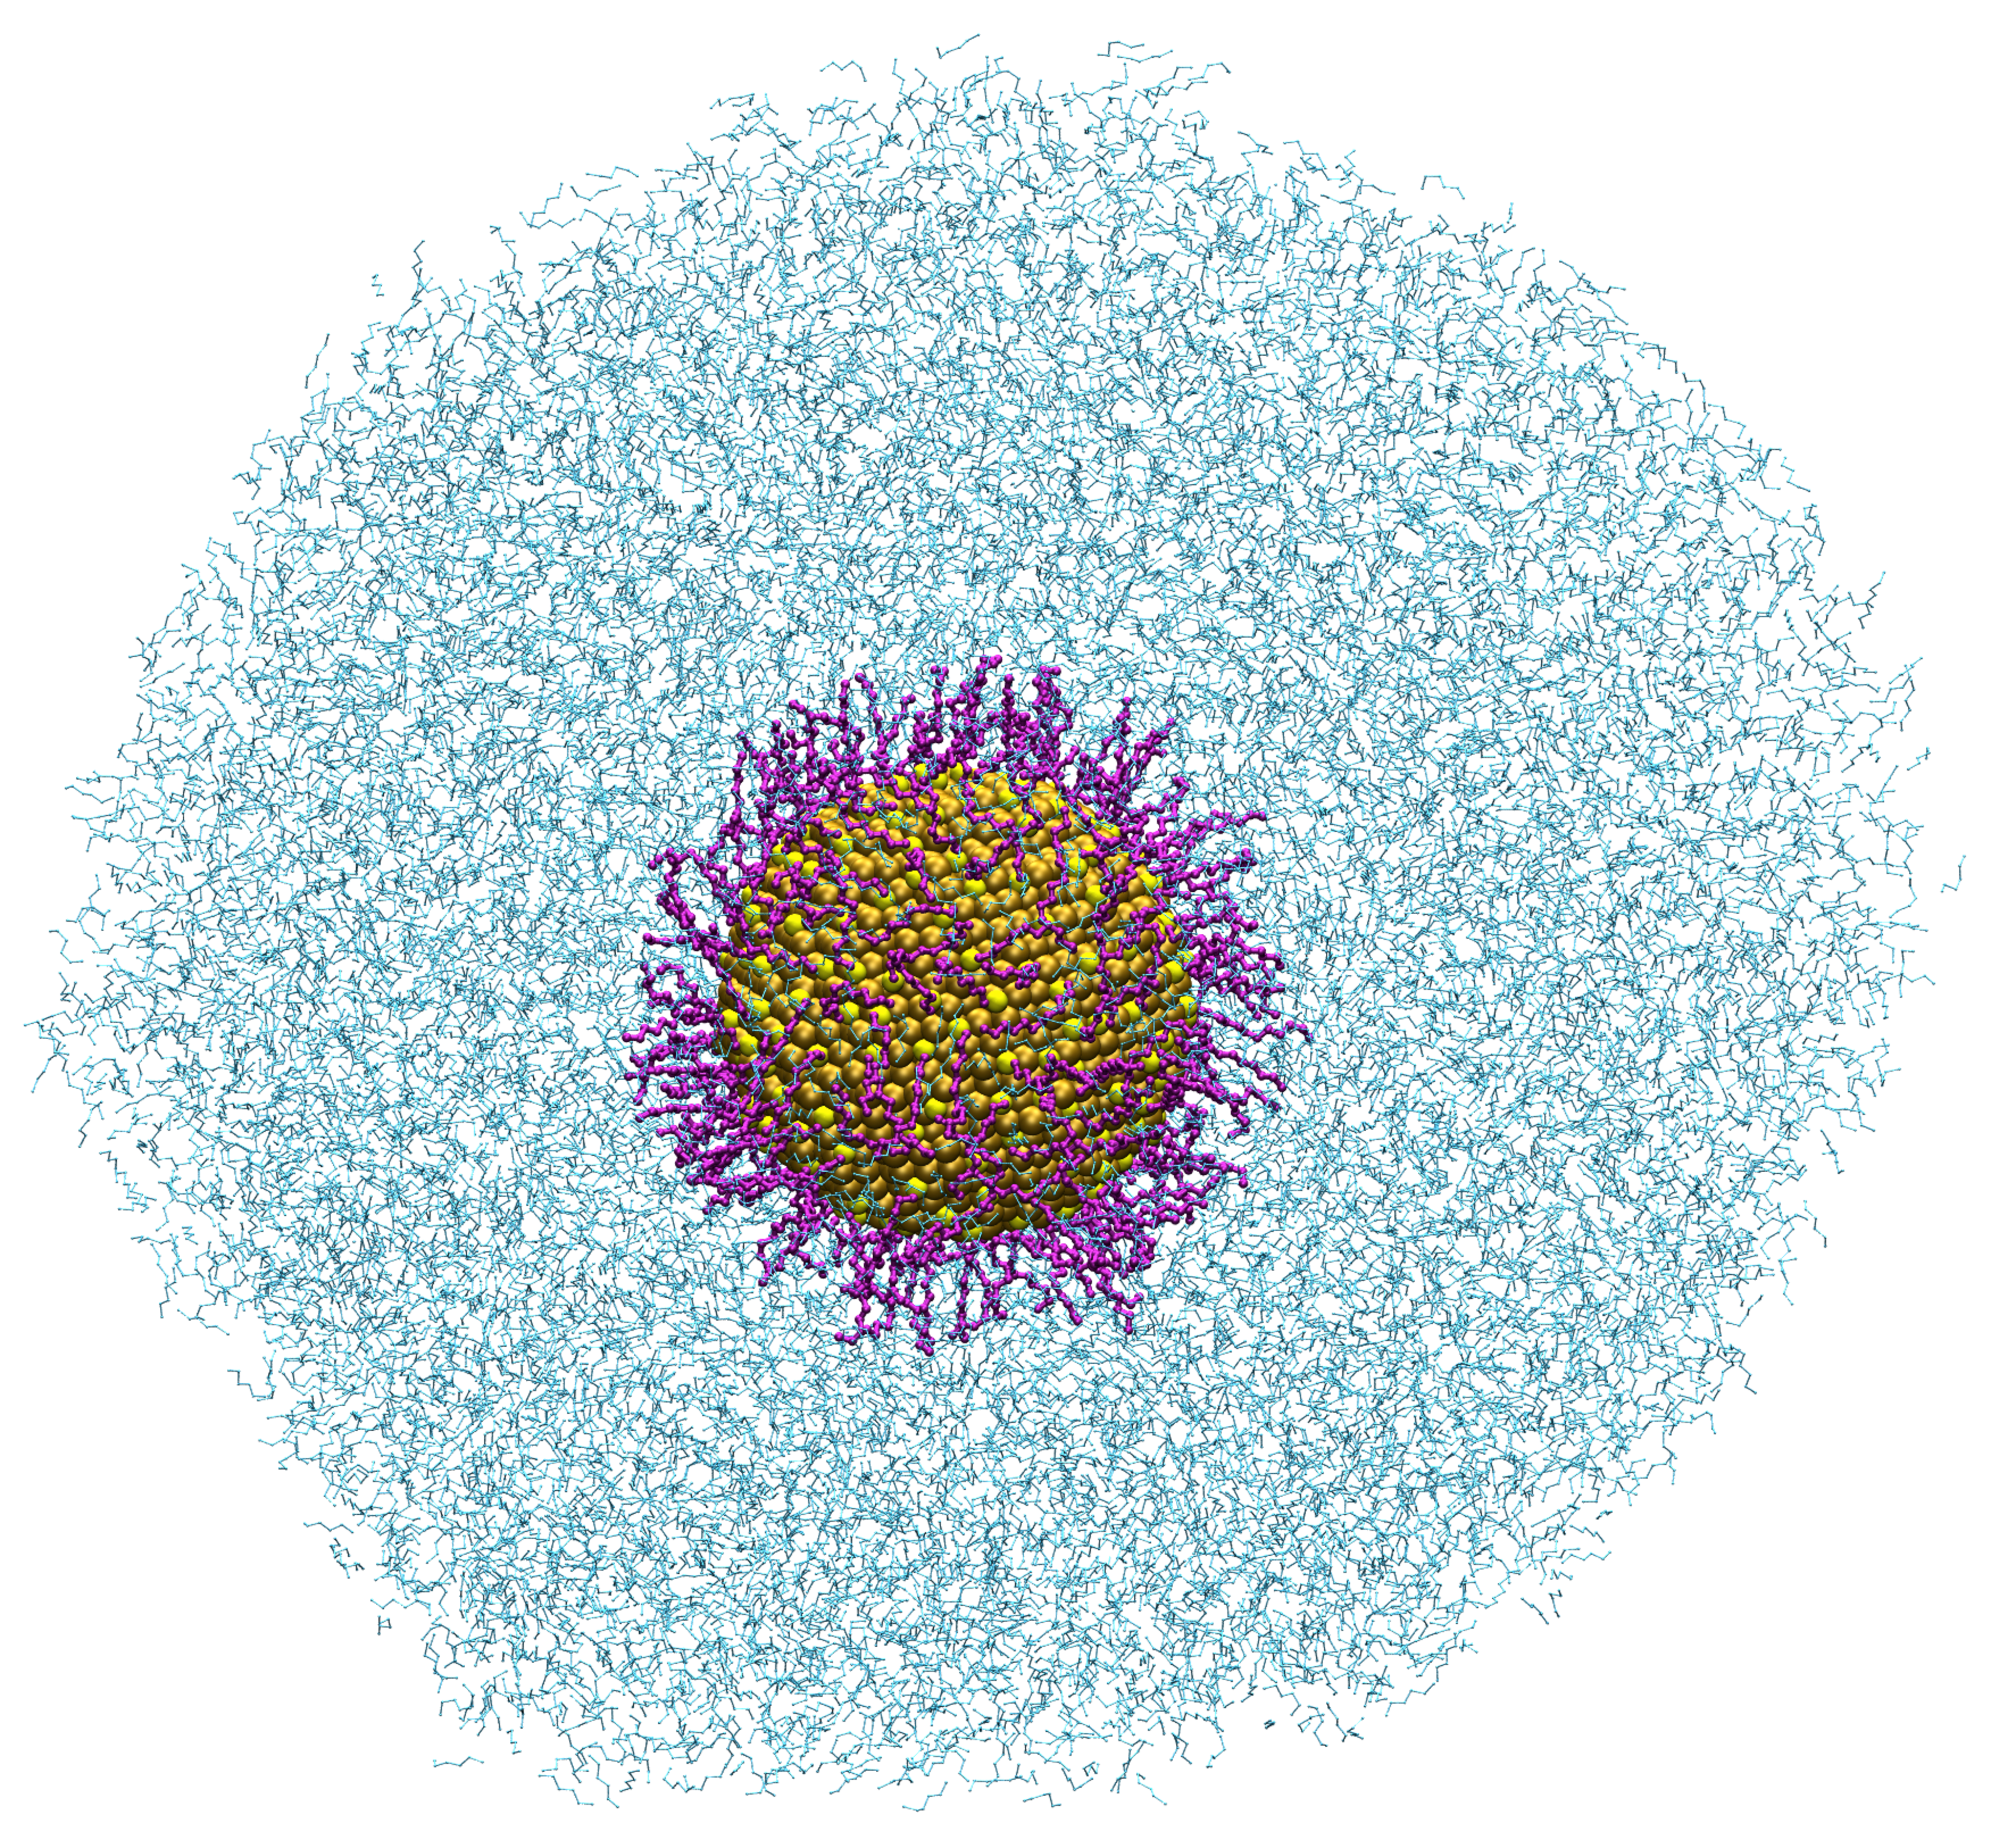
\includegraphics[width=\linewidth]{figures/NP25_C12h1}
  \caption{A 25 \AA\ radius gold nanoparticle protected with a
    half-monolayer of TraPPE-UA dodecanethiolate (C$_{12}$) ligands
    and solvated in TraPPE-UA hexane. The interfacial thermal
    conductance is computed by applying a kinetic energy flux between
    the nanoparticle and an outer shell of solvent.}
  \label{fig:NP25_C12h1}
\end{figure}

Once equilibrated, thermal fluxes were applied for 1 ns, until stable
temperature gradients had developed (see figure
\ref{fig:temp_profile}). Systems were run under moderate pressure (50
atm) with an average temperature (250K) that maintained a compact
solvent cluster and avoided formation of a vapor layer near the heated
metal surface.  Pressure was applied to the system via the
non-periodic ``Langevin Hull'' algorithm.\cite{Vardeman2011} However,
thermal coupling to the external temperature bath was removed to avoid
interference with the imposed RNEMD flux.

\begin{figure}
	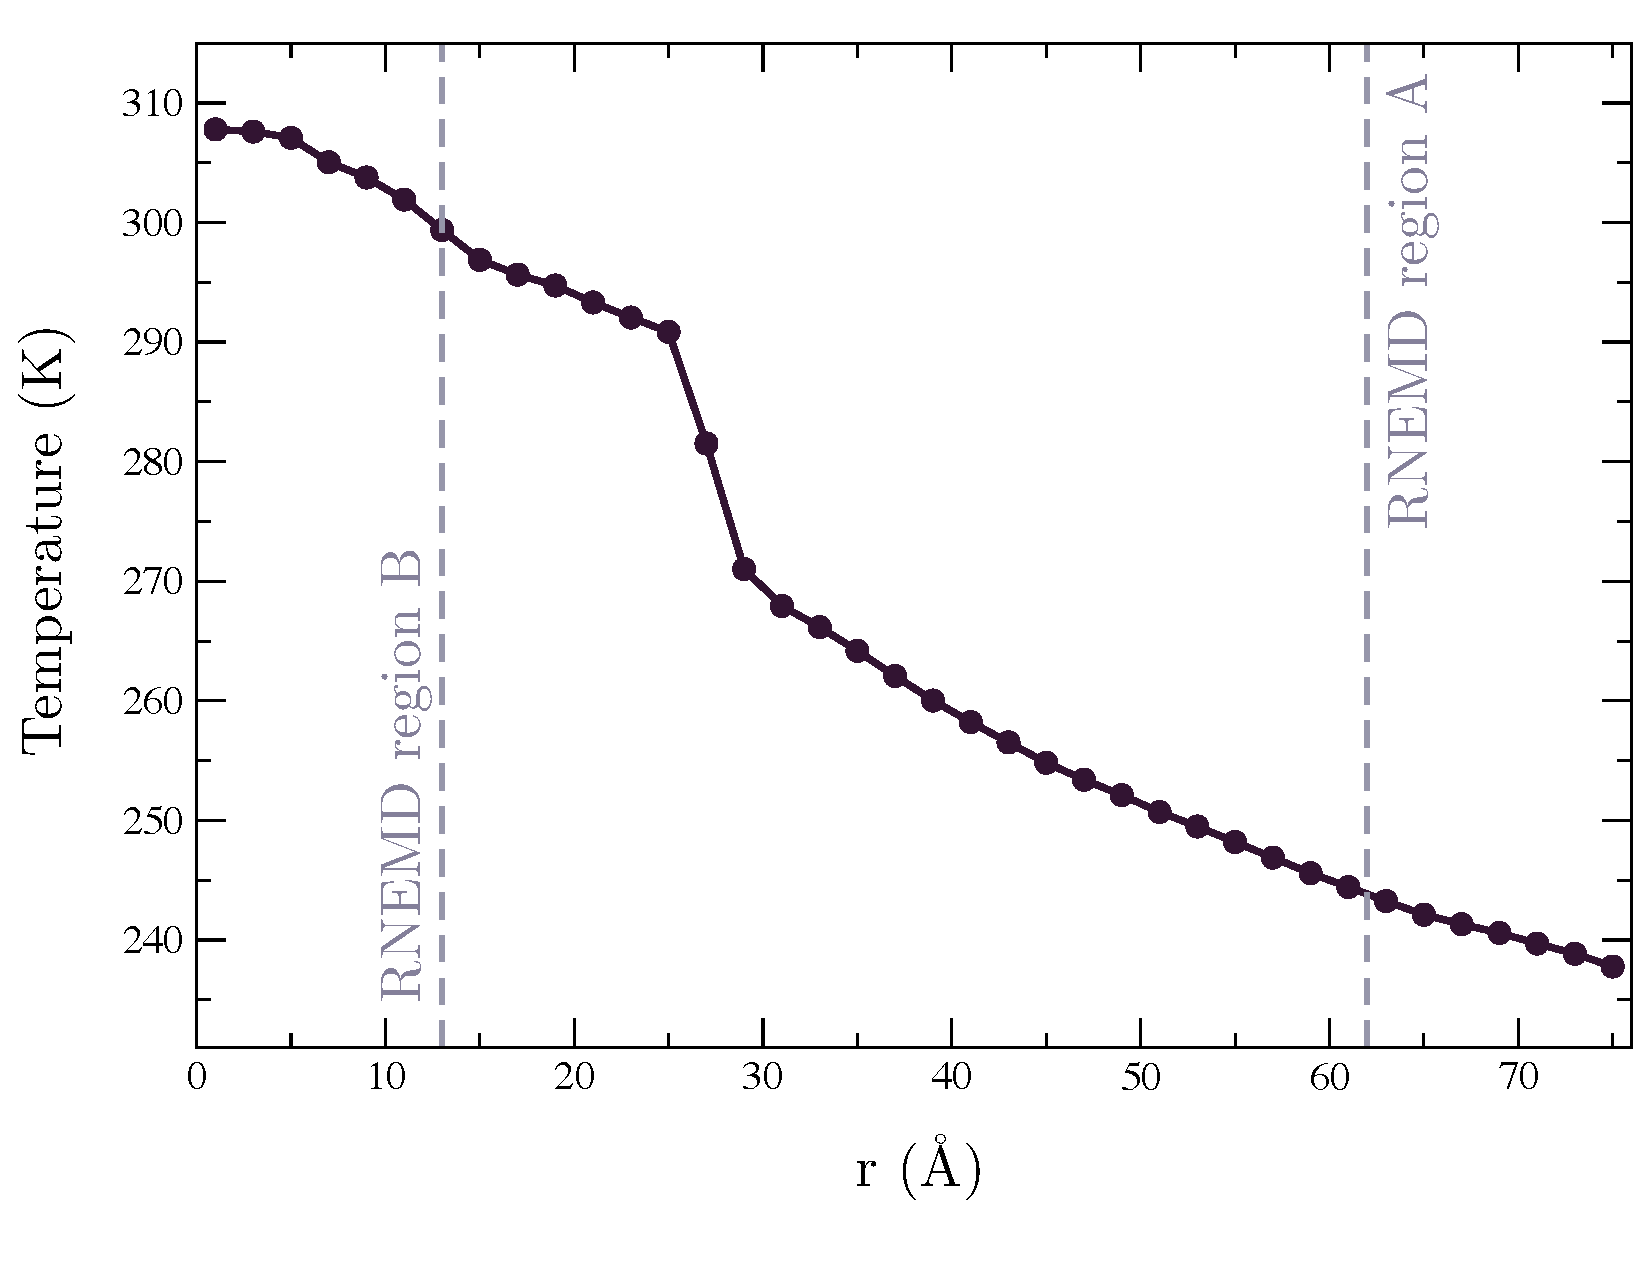
\includegraphics[width=\linewidth]{figures/temp_profile}
	\caption{Radial temperature profile for a 25 \AA\ radius
          particle protected with a 50\% coverage of TraPPE-UA
          butanethiolate (C$_4$) ligands and solvated in TraPPE-UA
          hexane. A kinetic energy flux is applied between RNEMD
          region A and RNEMD region B. The size of the temperature
          discontinuity at the interface is governed by the
          interfacial thermal conductance.}
	\label{fig:temp_profile}
\end{figure}

Although the VSS-RNEMD moves conserve \emph{total} angular momentum
and energy, systems which contain a metal nanoparticle embedded in a
significant volume of solvent will still experience nanoparticle
diffusion inside the solvent droplet. To aid in measuring an accurate
temperature profile for these systems, a single gold atom at the
origin of the coordinate system was assigned a mass $10,000 \times$
its original mass. The bonded and nonbonded interactions for this atom
remain unchanged and the heavy atom is excluded from the RNEMD
velocity scaling.  The only effect of this gold atom is to effectively
pin the nanoparticle at the origin of the coordinate system, thereby
preventing translational diffusion of the nanoparticle due to Brownian
motion.

To provide statistical independence, five separate configurations were
simulated for each particle radius and ligand. The structures were
unique, starting at the point of ligand placement, in order to sample
multiple surface-ligand configurations.


%%%%%%%%%%%%%%%%%%%%%%%%%%%%%%%%%%%%%%%%%%%%%%%%%%%%%%%%%%%%%%%%%%%%%%%%%%%%%%%%%%%
%		EFFECT OF PARTICLE SIZE
%%%%%%%%%%%%%%%%%%%%%%%%%%%%%%%%%%%%%%%%%%%%%%%%%%%%%%%%%%%%%%%%%%%%%%%%%%%%%%%%%%%
\section{Results}

We modeled four sizes of nanoparticles ($R =$ 10, 15, 20, and 25
\AA). The smallest particle size produces the lowest interfacial
thermal conductance values for most of the of protecting groups
(Fig. \ref{fig:NPthiols_G}).  Between the other three sizes of
nanoparticles, there is no systematic dependence of the interfacial
thermal conductance on the nanoparticle size. It is likely that the
differences in local curvature of the nanoparticle sizes studied here
do not disrupt the ligand packing and behavior in drastically
different ways.

\begin{figure}
  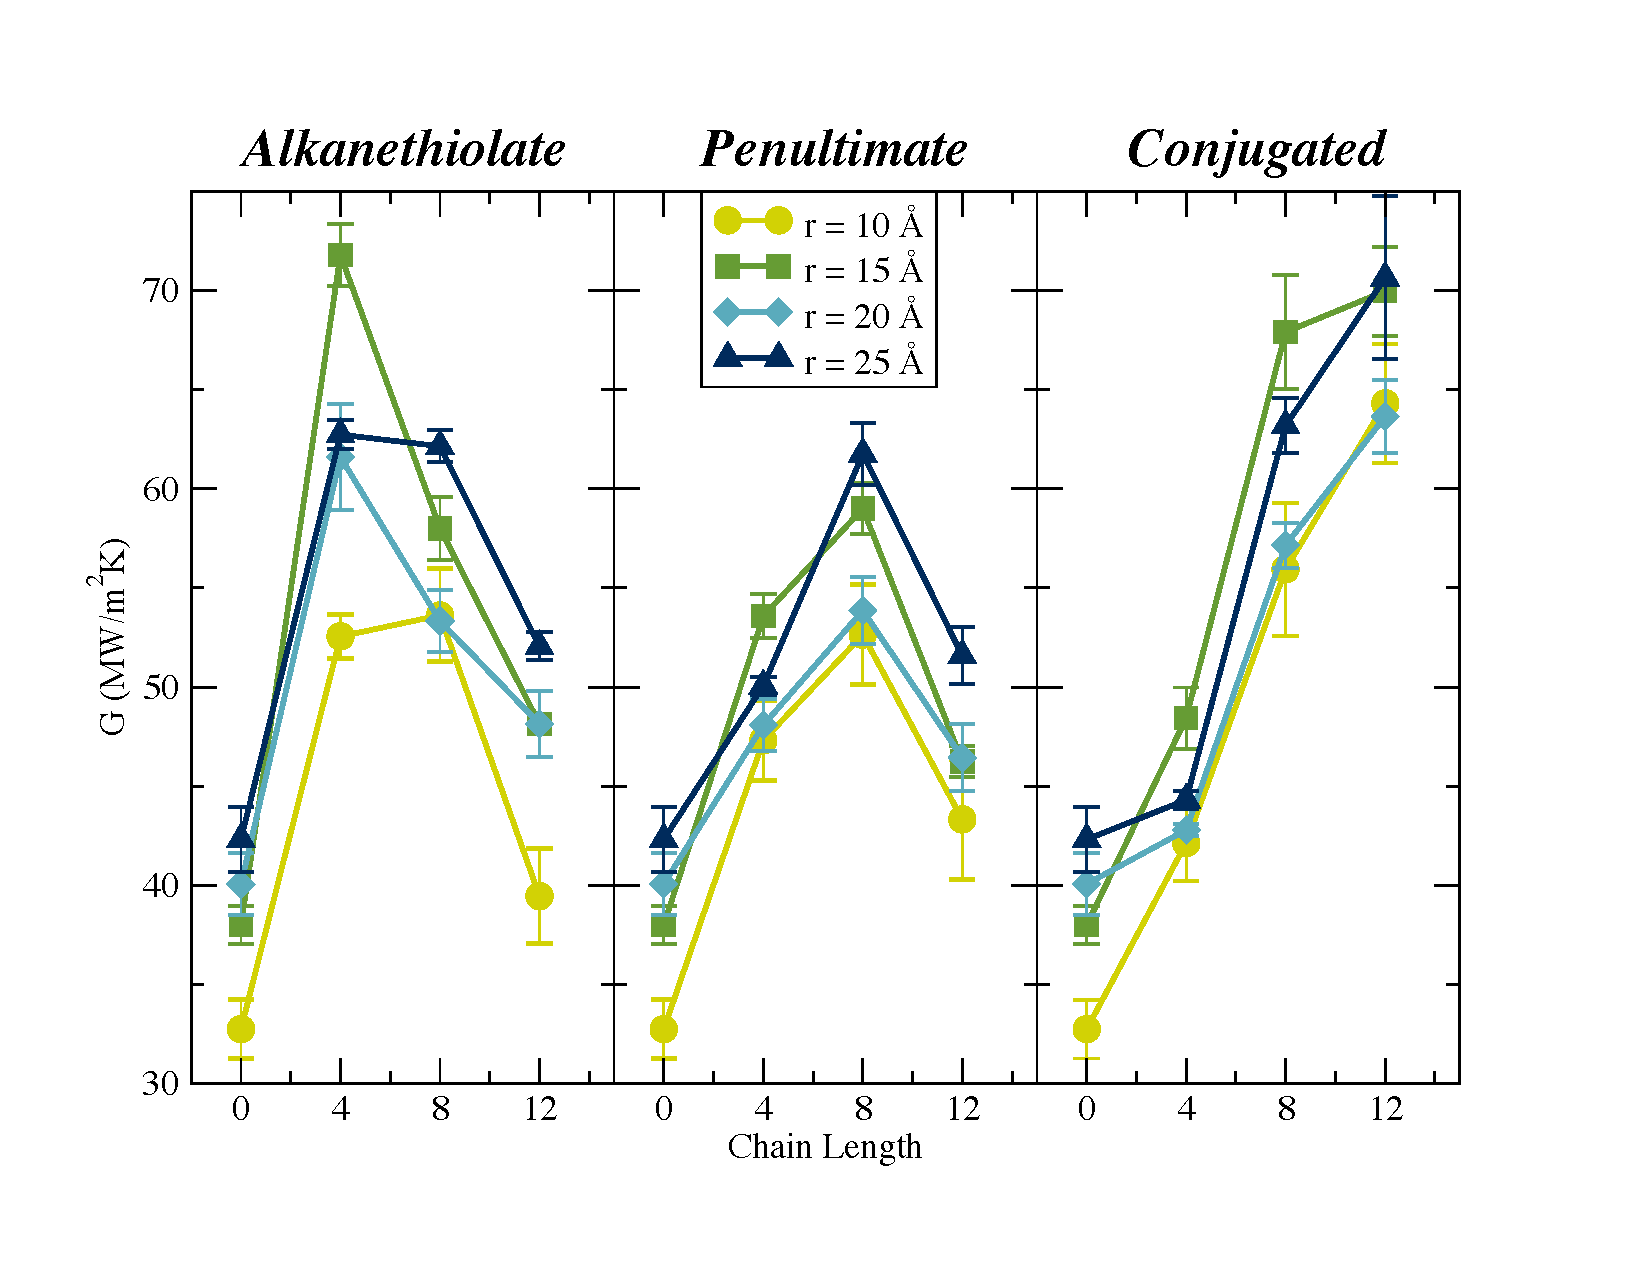
\includegraphics[width=\linewidth]{figures/G3}
  \caption{Interfacial thermal conductance ($G$) values for 4
      sizes of solvated nanoparticles that are bare or protected with
      a 50\% coverage of C$_{4}$, C$_{8}$, or C$_{12}$ thiolate
      ligands. Ligands of different flexibility are shown in separate
      panels.  The middle panel indicates ligands which have a single
      carbon-carbon double bond in the penultimate position.}
  \label{fig:NPthiols_G}
\end{figure}

%%%%%%%%%%%%%%%%%%%%%%%%%%%%%%%%%%%%%%%%%%%%%%%%%%%%%%%%%%%%%%%%%%%%%%%%%%%%%%%%%%%
%		EFFECT OF LIGAND CHAIN LENGTH
%%%%%%%%%%%%%%%%%%%%%%%%%%%%%%%%%%%%%%%%%%%%%%%%%%%%%%%%%%%%%%%%%%%%%%%%%%%%%%%%%%%

Unlike a previous study of varying thiolate ligand chain lengths on
planar Au(111) surfaces, the interfacial thermal conductance of
ligand-protected nanospheres exhibits a distinct dependence on the
ligand identity.\cite{} A half-monolayer coverage of ligands yields
interfacial conductance that is strongly dependent on both ligand
length and flexibility.

There are many factors that could be playing a role in the
ligand-dependent conductuance.  The sulfur-gold interaction is
particularly strong, and the presence of the ligands can easily
disrupt the crystalline structure of the gold at the surface of the
particles, providing more efficient scattering of phonons into the
ligand / solvent layer. This effect would be particularly important at
small particle sizes.

\texit{In previous studies of mixed-length ligand layers with full coverage,
we observed that ligand-solvent alignment was an important factor for
heat transfer into the solvent.  With high surface curvature and lower
effective coverages, ligand behavior also becomes more complex. Some
chains may be lying down on the surface, and solvent may not be
penetrating the ligand layer to the same degree as in the planar
surfaces.
}  

Additionally, the ligand flexibility directly alters the vibrational
density of states for the layer that mediates the transfer of phonons
between the metal and the solvent. This could be a partial explanation
for the observed differences between the fully conjugated and more
flexible ligands.

In the following sections details on how I
measure surface corrugation, solvent-ligand interpenetration, and
ordering of the solvent and ligand at the surfaces of the
nanospheres are provided. Followed by an investigation of 
the overlap between vibrational densities of states for the various ligands.

%%%%%%%%%%%%%%%%%%%%%%%%%%%%%%%%%%%%%%%%%%%%%%%%%%%%%%%%%%%%%%%%%%%%%%%%%%%%%%%%%%%
%		CORRUGATION OF PARTICLE SURFACE
%%%%%%%%%%%%%%%%%%%%%%%%%%%%%%%%%%%%%%%%%%%%%%%%%%%%%%%%%%%%%%%%%%%%%%%%%%%%%%%%%%%
\subsection{Corrugation of the Particle Surface}

The bonding sites for thiols on gold surfaces have been studied
extensively and include configurations beyond the traditional atop,
bridge, and hollow sites found on planar surfaces. In particular, the
deep potential well between the gold atoms and the thiolate sulfur
atoms leads to insertion of the sulfur into the gold lattice and
displacement of interfacial gold atoms. The degree of ligand-induced
surface restructuring may have an impact on the interfacial thermal
conductance and is an important phenomenon to quantify.

Henz, \textit{et al.}\cite{Henz:2008qf} used the metal
density as a function of radius to measure the degree of mixing
between the thiol sulfurs and surface gold atoms at the edge of a
nanoparticle. Although metal density is important, disruption of the
local crystalline ordering would also have a large effect on the
phonon spectrum in the particles. To measure this effect, the
fraction of gold atoms exhibiting local fcc ordering as a function of
radius to describe the ligand-induced disruption of the nanoparticle
surface is used.

The local bond orientational order can be described using the method
of Steinhardt \textit{et al.}\cite{Steinhardt1983} The local bonding
environment, $\bar{q}_{\ell m}$, for each atom in the system is
determined by averaging over the spherical harmonics between that atom
and each of its neighbors,
\begin{equation}
\bar{q}_{\ell m} = \sum_i Y_\ell^m(\theta_i, \phi_i)
\end{equation}
where $\theta_i$ and $\phi_i$ are the relative angular coordinates of
neighbor $i$ in the laboratory frame.  A global average orientational
bond order parameter, $\bar{Q}_{\ell m}$, is the average over each
$\bar{q}_{\ell m}$ for all atoms in the system. To remove the
dependence on the laboratory coordinate frame, the third order
rotationally invariant combination of $\bar{Q}_{\ell m}$,
$\hat{w}_\ell$, is utilized here.\cite{Steinhardt1983,Vardeman:2008fk}

For $\ell=4$, the ideal face-centered cubic (fcc), body-centered cubic
(bcc), hexagonally close-packed (hcp), and simple cubic (sc) local
structures exhibit $\hat{w}_4$ values of -0.159, 0.134, 0.159, and
0.159, respectively. Because $\hat{w}_4$ exhibits an extreme value for
fcc structures, it is ideal for measuring local fcc
ordering. The spatial distribution of $\hat{w}_4$ local bond
orientational order parameters, $p(\hat{w}_4 , r)$, can provide
information about the location of individual atoms that are central to
local fcc ordering.

The fraction of fcc-ordered gold atoms at a given radius in the
nanoparticle,
\begin{equation}
	f_\mathrm{fcc}(r) = \int_{-\infty}^{w_c} p(\hat{w}_4, r) d \hat{w}_4
\end{equation}
is described by the distribution of the local bond orientational order
parameters, $p(\hat{w}_4, r)$, and $w_c$, a cutoff for the peak
$\hat{w}_4$ value displayed by fcc structures. A $w_c$ value of -0.12
was chosen to isolate the fcc peak in $\hat{w}_4$.

As illustrated in Figure \ref{fig:Corrugation}, the presence of
ligands decreases the fcc ordering of the gold atoms at the
nanoparticle surface. For the smaller nanoparticles, this disruption
extends into the core of the nanoparticle, indicating widespread
disruption of the lattice.

\begin{figure}
  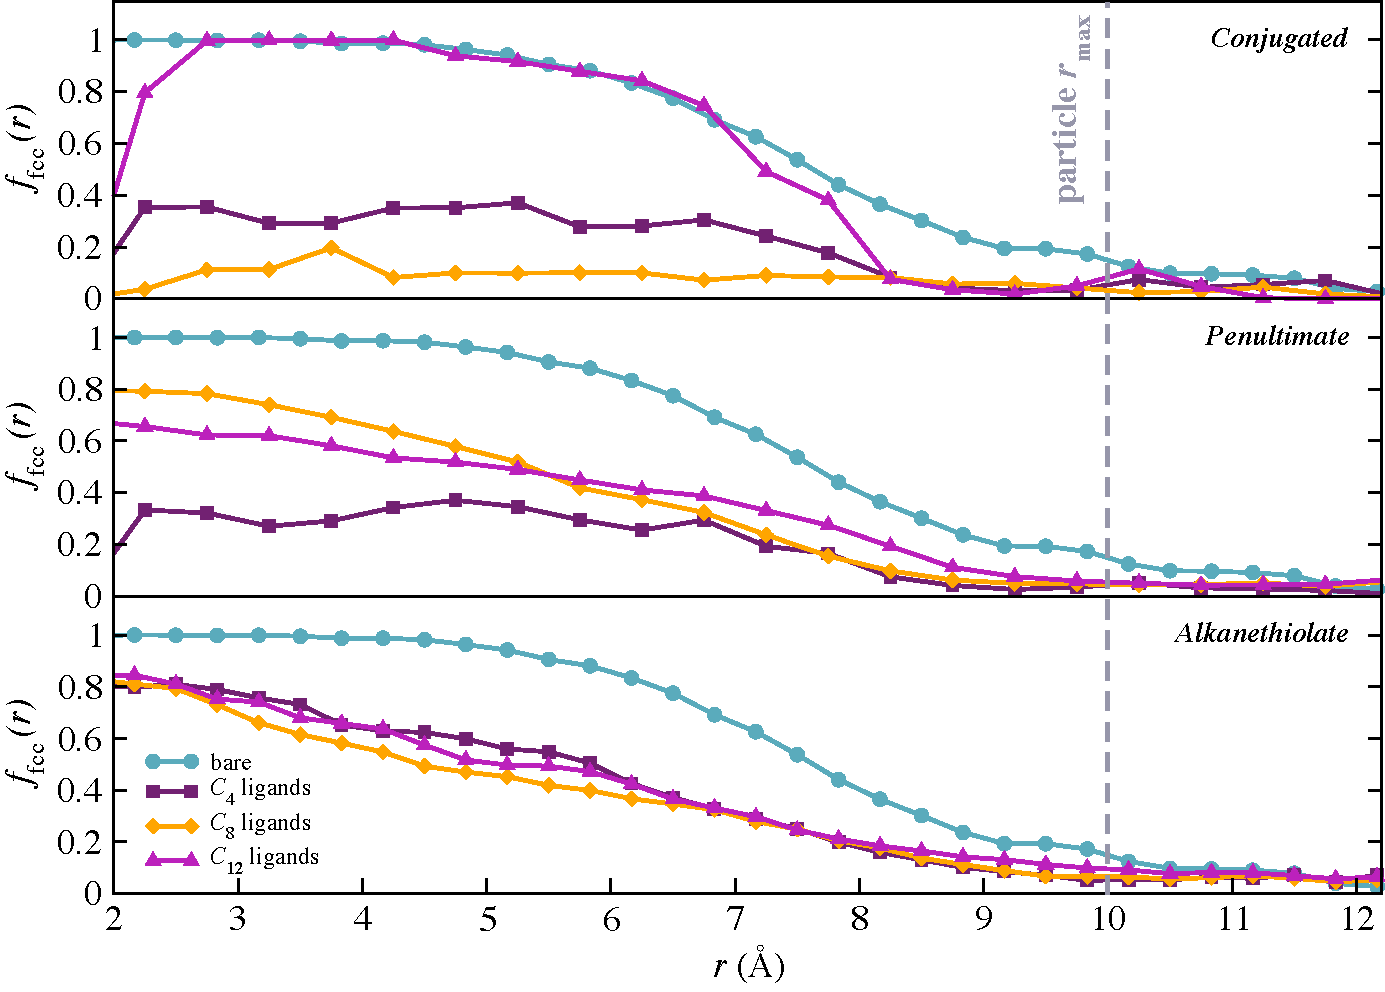
\includegraphics[width=\linewidth]{figures/fcc}
  \caption{Fraction of gold atoms with fcc ordering as a function of
    radius for a 10 \AA\ radius nanoparticle. The decreased fraction
    of fcc-ordered atoms in ligand-protected nanoparticles relative to
    bare particles indicates restructuring of the nanoparticle surface
    by the thiolate sulfur atoms.}
  \label{fig:Corrugation}
\end{figure}

The thickness of the disrupted nanoparticle surface can be described by
defining a corrugation factor, $c$, as the ratio of the radius at
which the fraction of gold atoms with fcc ordering is 0.9 and the
radius at which the fraction is 0.5.

\begin{equation}
	c = 1 - \frac{r(f_\mathrm{fcc} = 0.9)}{r(f_\mathrm{fcc} = 0.5)}
\end{equation}

A sharp interface will have a steep drop in $f_\mathrm{fcc}$ at the
edge of the particle ($c \rightarrow$ 0). In the opposite limit where
the entire nanoparticle surface is restructured by ligands, the radius
at which there is a high probability of fcc ordering moves
dramatically inward ($c \rightarrow$ 1).

The computed corrugation factors are shown in Figure
\ref{fig:NPthiols_corrugation} for bare nanoparticles and for
ligand-protected particles as a function of ligand chain length. The
largest nanoparticles are only slightly restructured by the presence
of ligands on the surface, while the smallest particle ($r$ = 10 \AA)
exhibits significant disruption of the original fcc ordering when
covered with a half-monolayer of thiol ligands.

\begin{figure}
  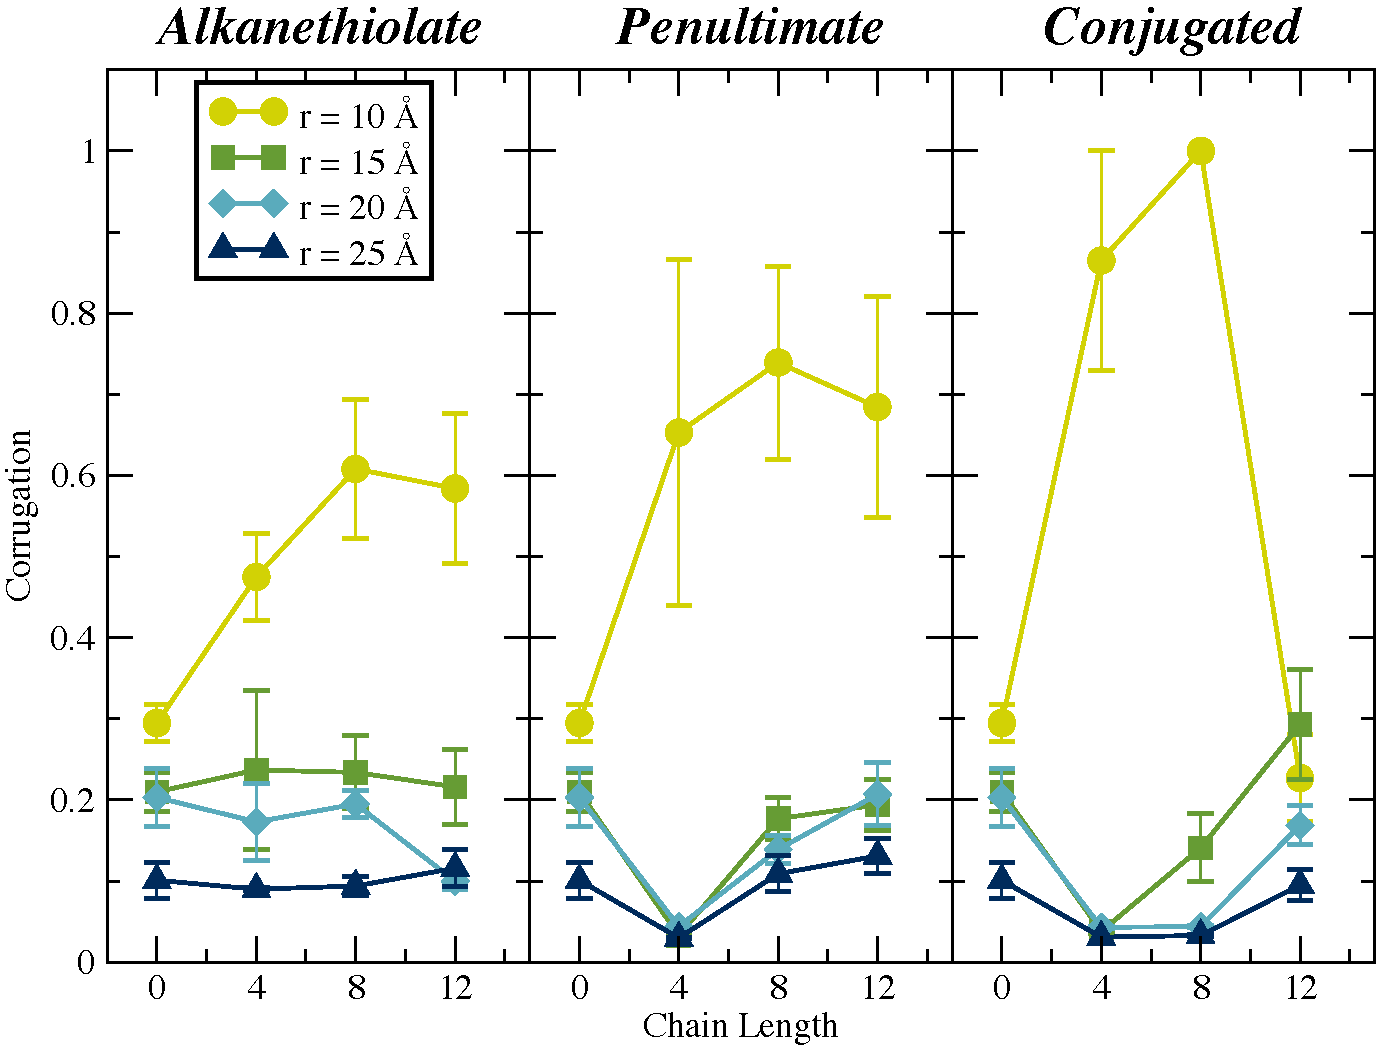
\includegraphics[width=\linewidth]{figures/C3.pdf}
  \caption{Computed corrugation values for 4 sizes of solvated
    nanoparticles that are bare or protected with a 50\% coverage of
    C$_{4}$, C$_{8}$, or C$_{12}$ thiolate ligands.  The smallest (10
    \AA ) particles show significant disruption to their crystal
    structures, and the length and stiffness of the ligands is a
    contributing factor to the surface disruption.}
  \label{fig:NPthiols_corrugation}
\end{figure}

Since the thiolate ligands do not significantly alter the larger
particle crystallinity, the surface corrugation does not seem to be a
likely candidate to explain the large increase in thermal conductance
at the interface when ligands are added.

% \begin{equation}
% 	C = \frac{r_{bare}(\rho_{\scriptscriptstyle{0.85}}) - r_{capped}(\rho_{\scriptscriptstyle{0.85}})}{r_{bare}(\rho_{\scriptscriptstyle{0.85}})}.
% \end{equation}
% 
% Here, $r_{bare}(\rho_{\scriptscriptstyle{0.85}})$ is the radius of a bare nanoparticle at which the density is $85\%$ the bulk value and $r_{capped}(\rho_{\scriptscriptstyle{0.85}})$ is the corresponding radius for a particle of the same size with a layer of ligands. $C$ has a value of 0 for a bare particle and approaches $1$ as the degree of surface atom mixing increases.




%%%%%%%%%%%%%%%%%%%%%%%%%%%%%%%%%%%%%%%%%%%%%%%%%%%%%%%%%%%%%%%%%%%%%%%%%%%%%%%%%%%
%		MOBILITY OF INTERFACIAL SOLVENT
%%%%%%%%%%%%%%%%%%%%%%%%%%%%%%%%%%%%%%%%%%%%%%%%%%%%%%%%%%%%%%%%%%%%%%%%%%%%%%%%%%%
% \subsection{Mobility of Interfacial Solvent}

% Another possible mechanism for increasing interfacial conductance is
% the mobility of the interfacial solvent.  We used a survival
% correlation function, $C(t)$, to measure the residence time of a
% solvent molecule in the nanoparticle thiolate
% layer.\cite{Stocker:2013cl} This function correlates the identity of
% all hexane molecules within the radial range of the thiolate layer at
% two separate times. If the solvent molecule is present at both times,
% the configuration contributes a $1$, while the absence of the molecule
% at the later time indicates that the solvent molecule has migrated
% into the bulk, and this configuration contributes a $0$. A steep decay
% in $C(t)$ indicates a high turnover rate of solvent molecules from the
% chain region to the bulk. We may define the escape rate for trapped
% solvent molecules at the interface as
% \begin{equation}
%  k_\mathrm{escape} = \left( \int_0^T C(t) dt \right)^{-1}
%   \label{eq:mobility}
% \end{equation}
% where T is the length of the simulation. This is a direct measure of
% the rate at which solvent molecules initially entangled in the
% thiolate layer can escape into the bulk. When $k_\mathrm{escape}
% \rightarrow 0$, the solvent becomes permanently trapped in the
% interfacial region.

% The solvent escape rates for bare and ligand-protected nanoparticles
% are shown in Figure \ref{fig:NPthiols_combo}. As the ligand chain
% becomes longer and more flexible, interfacial solvent molecules become
% trapped in the ligand layer and the solvent escape rate decreases.
% This mechanism contributes a partial explanation as to why the longer
% ligands have significantly lower thermal conductance.

%%%%%%%%%%%%%%%%%%%%%%%%%%%%%%%%%%%%%%%%%%%%%%%%%%%%%%%%%%%%%%%%%%%%%%%%%%%%%%%%%%%
%		ORIENTATION OF LIGAND CHAINS
%%%%%%%%%%%%%%%%%%%%%%%%%%%%%%%%%%%%%%%%%%%%%%%%%%%%%%%%%%%%%%%%%%%%%%%%%%%%%%%%%%%
\subsection{Orientation of Ligand Chains}

Previous theoretical work on heat conduction through alkane chains has
shown that short chains are dominated by harmonic interactions, where
the energy is carried ballistically through the
chain.\cite{Segal:2003qy} As the saturated ligand chain length
increases in length, it exhibits significantly more conformational
flexibility. Thus, different lengths of ligands should favor different
chain orientations on the surface of the nanoparticle, and can
localize the ligand vibrational density of states close to the
particle, lowering the effectiveness of the heat
conduction.\cite{Segal:2003qy} To determine the distribution of ligand
orientations relative to the particle surface the 
probability of finding a ligand with a particular orientation relative
to the surface normal of the nanoparticle is examined,
\begin{equation} 
\cos{(\theta)}=\frac{\vec{r}_i\cdot\hat{u}_i}{|\vec{r}_i||\hat{u}_i|}
\end{equation}
where $\vec{r}_{i}$ is the vector between the cluster center of mass
and the sulfur atom on ligand molecule {\it i}, and $\hat{u}_{i}$ is
the  vector between the sulfur atom and \ce{CH3} pseudo-atom on ligand
molecule {\it i}. As depicted in Figure \ref{fig:NP_pAngle}, $\theta
\rightarrow 180^{\circ}$ for a ligand chain standing upright on the
particle ($\cos{(\theta)} \rightarrow -1$) and $\theta \rightarrow
90^{\circ}$ for a ligand chain lying down on the surface
($\cos{(\theta)} \rightarrow 0$). As the thiolate alkane chain
increases in length and becomes more flexible, the ligands are more
willing to lie down on the nanoparticle surface and exhibit increased
population at $\cos{(\theta)} = 0$.

\begin{figure}
  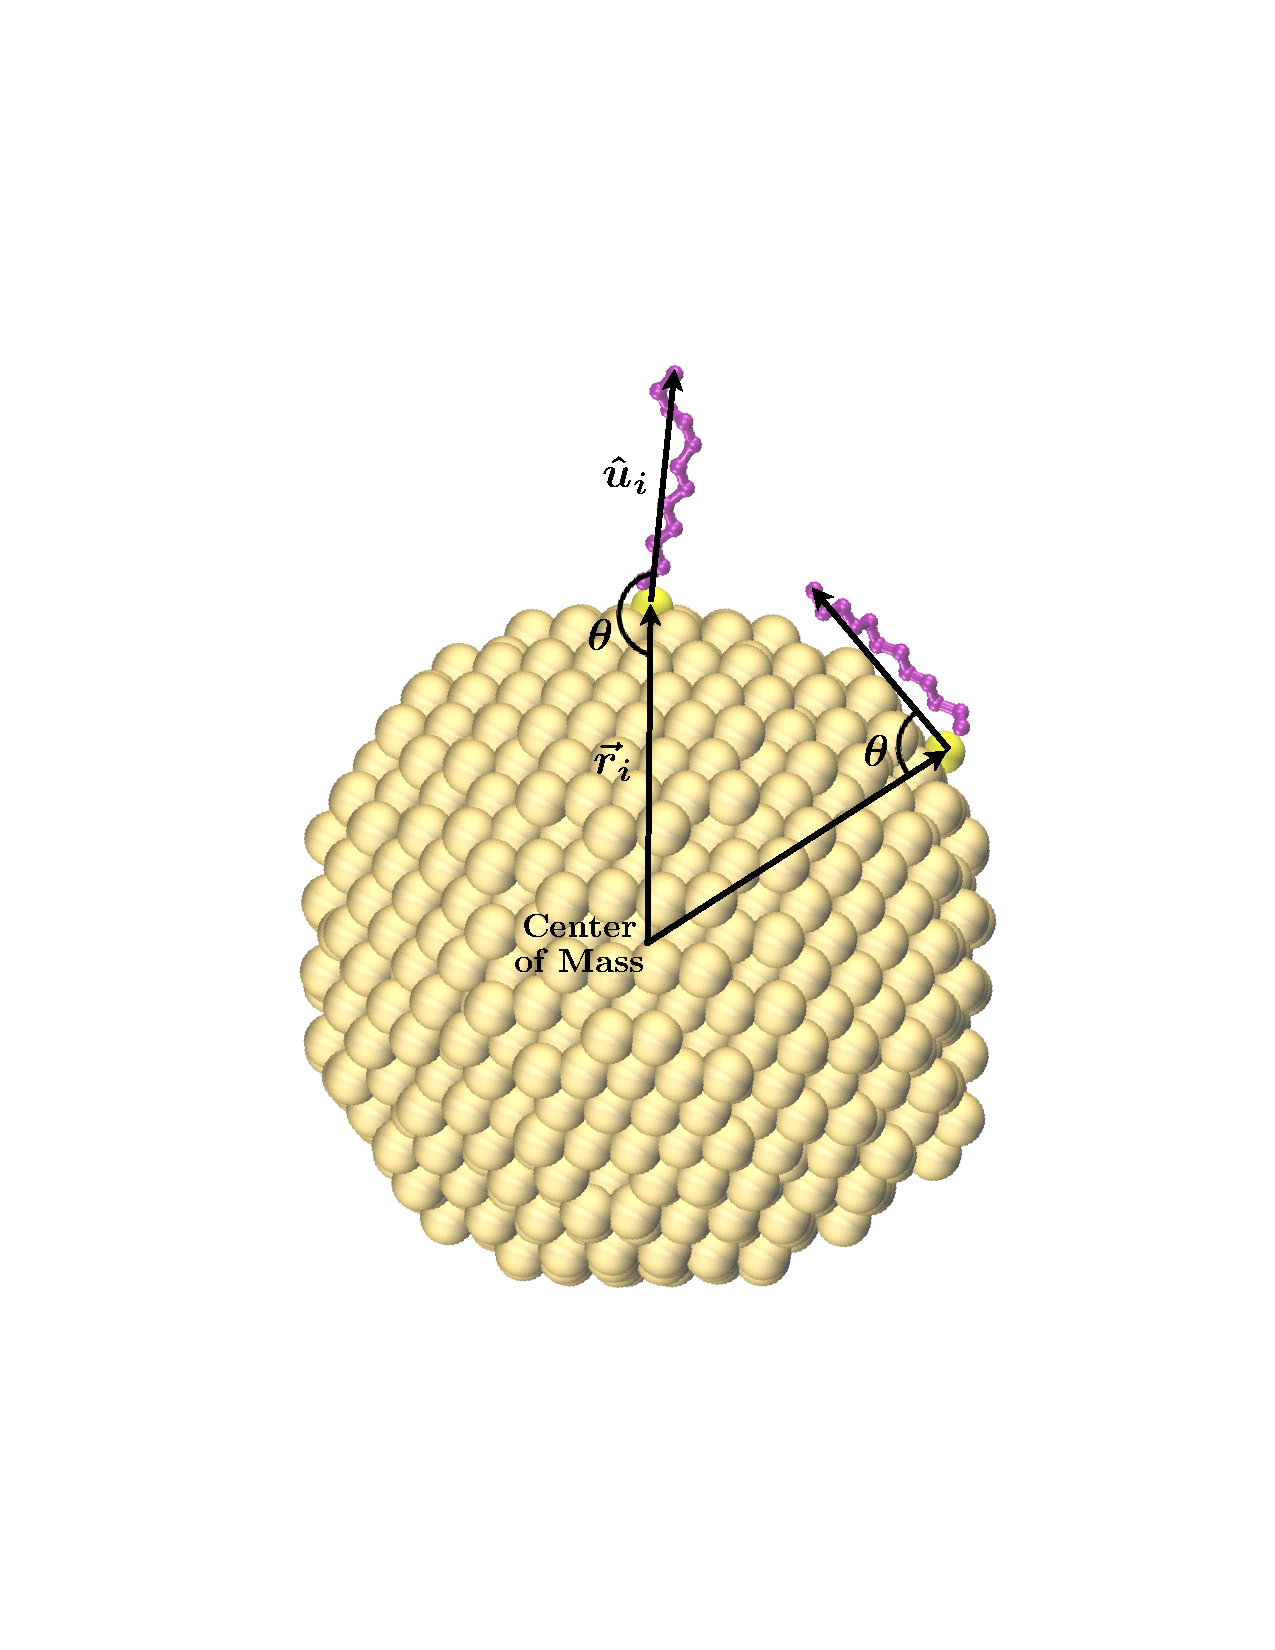
\includegraphics[width=\linewidth]{figures/NP_pAngle}
  \caption{The two extreme cases of ligand orientation relative to the
    nanoparticle surface: the ligand completely outstretched
    ($\cos{(\theta)} = -1$) and the ligand fully lying down on the
    particle surface ($\cos{(\theta)} = 0$).}
  \label{fig:NP_pAngle}
\end{figure}

An order parameter describing the average ligand chain orientation relative to
the nanoparticle surface is available using the second order Legendre
parameter,
\begin{equation}
	P_2 = \left< \frac{1}{2} \left(3\cos^2(\theta) - 1 \right) \right>
\end{equation}

Ligand populations that are perpendicular to the particle surface have
$P_2$ values of 1, while ligand populations lying flat on the
nanoparticle surface have $P_2$ values of $-0.5$. Disordered ligand
layers will exhibit mean $P_2$ values of 0. As shown in Figure
\ref{fig:NPthiols_P2} the ligand $P_2$ values approaches 0 as
ligand chain length -- and ligand flexibility -- increases.

%%%%%%%%%%%%%%%%%%%%%%%%%%%%%%%%%%%%%%%%%%%%%%%%%%%%%%%%%%%%%%%%%%%%%%%%%%%%%%%%%%%
%		ORIENTATION OF INTERFACIAL SOLVENT
%%%%%%%%%%%%%%%%%%%%%%%%%%%%%%%%%%%%%%%%%%%%%%%%%%%%%%%%%%%%%%%%%%%%%%%%%%%%%%%%%%%
\subsection{Orientation of Interfacial Solvent}

Similarly, I examined the distribution of \emph{hexane} molecule
orientations relative to the particle surface using the same angular
analysis utilized for the ligand chain orientations. In this case,
$\vec{r}_i$ is the vector between the particle center of mass and one
of the \ce{CH2} pseudo-atoms in the middle of hexane molecule $i$ and
$\hat{u}_i$ is the vector between the two \ce{CH3} pseudo-atoms on
molecule $i$. Since only the orientation of
solvent molecules near the ligand layer is of interest, 
I select only the hexane
molecules within a specific $r$-range, between the edge of the
particle and the end of the ligand chains. A large population of
hexane molecules with $\cos{(\theta)} \sim \pm 1$ would indicate
interdigitation of the solvent molecules between the upright ligand
chains. A more random distribution of $\cos{(\theta)}$ values
indicates a disordered arrangement of solvent molecules near the particle
surface. Again, $P_2$ order parameter values provide a population
analysis for the solvent that is close to the particle surface.

The average orientation of the interfacial solvent molecules is
notably flat on the \emph{bare} nanoparticle surfaces. This blanket of
hexane molecules on the particle surface may act as an insulating
layer, increasing the interfacial thermal resistance. As the length
(and flexibility) of the ligand increases, the average interfacial
solvent P$_2$ value approaches 0, indicating a more random orientation
of the ligand chains. The average orientation of solvent within the
$C_8$ and $C_{12}$ ligand layers is essentially random. Solvent
molecules in the interfacial region of $C_4$ ligand-protected
nanoparticles do not lie as flat on the surface as in the case of the
bare particles, but are not as randomly oriented as the longer ligand
lengths.

\begin{figure}
  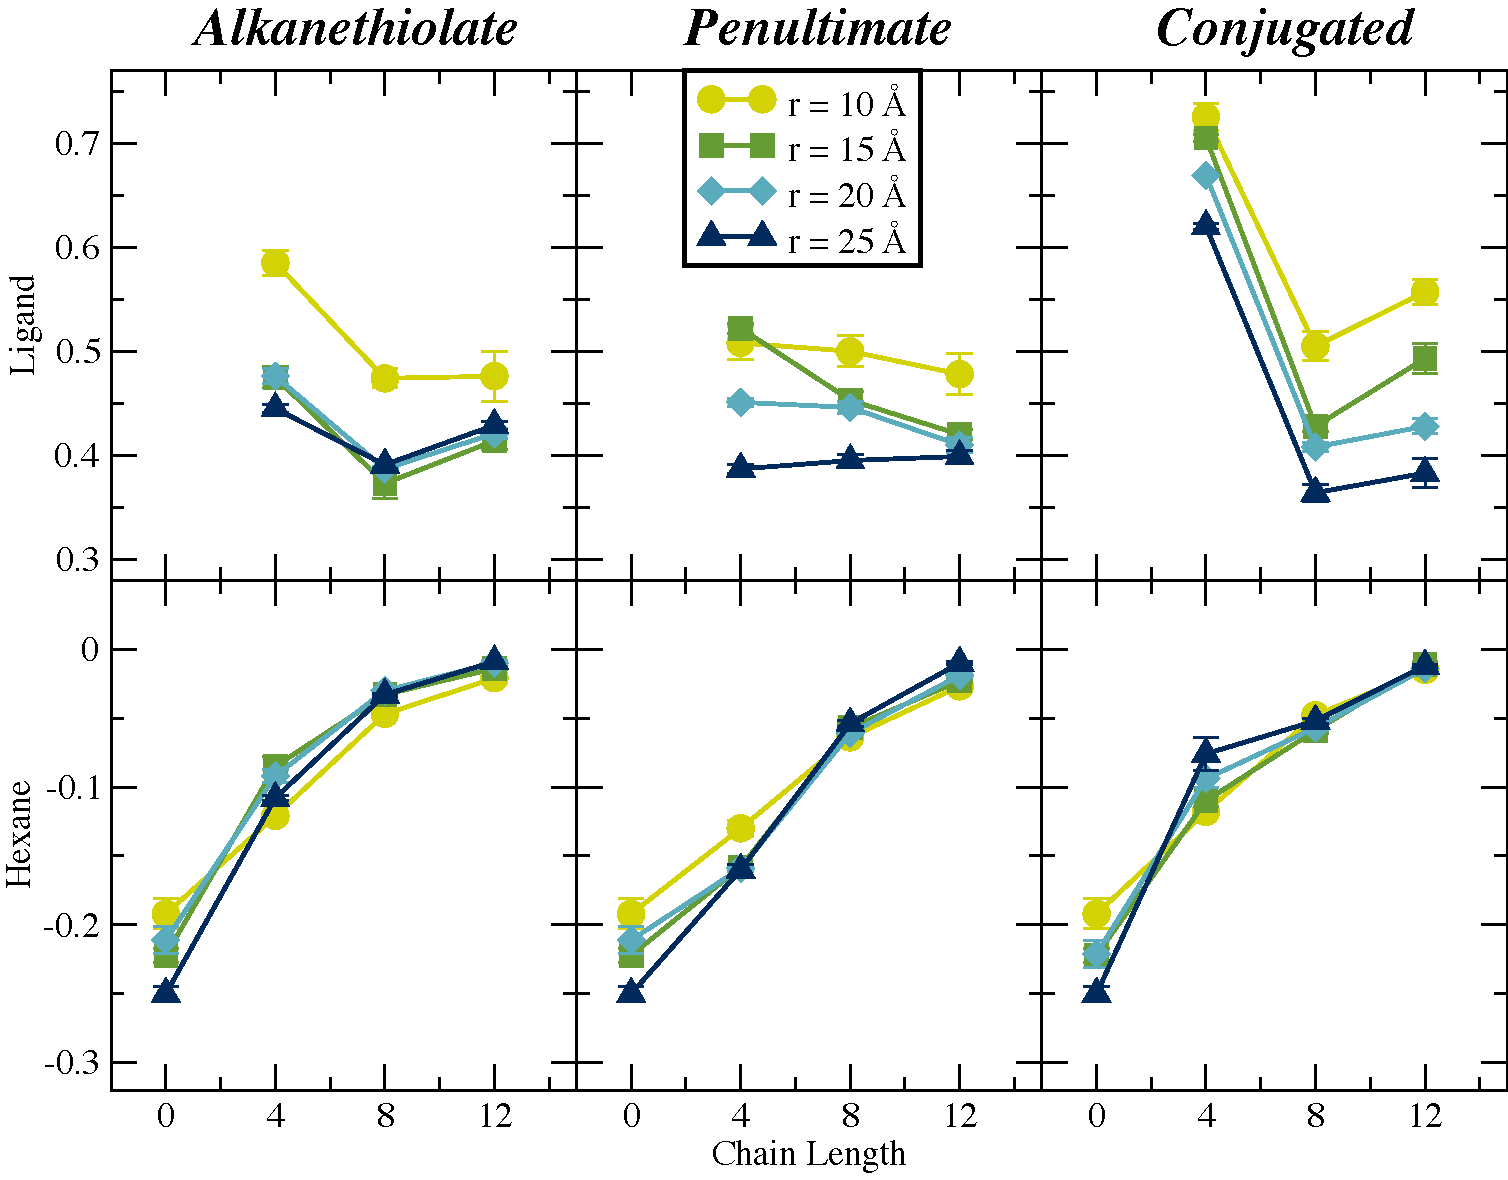
\includegraphics[width=\linewidth]{figures/P2_3.pdf}
  \caption{Computed ligand and interfacial solvent orientational $P_2$
    values for 4 sizes of solvated nanoparticles that are bare or
    protected with a 50\% coverage of C$_{4}$, C$_{8}$, or C$_{12}$
    alkanethiolate ligands. Increasing stiffness of the ligand orients
    these molecules normal to the particle surface, while the length
    of the ligand chains works to prevent solvent from lying flat on
    the surface.}
  \label{fig:NPthiols_P2}
\end{figure}

These results are particularly interesting in light of previous
work by Stocker \textit{et. al}\cite{Stocker:2013cl}, where solvent molecules readily filled
the vertical gaps between neighboring ligand chains and there was a
strong correlation between ligand and solvent molecular
orientations. It appears that the introduction of surface curvature
and a lower ligand packing density creates a disordered ligand layer
that lacks well-formed channels for the solvent molecules to occupy.

%%%%%%%%%%%%%%%%%%%%%%%%%%%%%%%%%%%%%%%%%%%%%%%%%%%%%%%%%%%%%%%%%%%%%%%%%%%%%%%%%%%
%		SOLVENT PENETRATION OF LIGAND LAYER
%%%%%%%%%%%%%%%%%%%%%%%%%%%%%%%%%%%%%%%%%%%%%%%%%%%%%%%%%%%%%%%%%%%%%%%%%%%%%%%%%%%
\subsection{Solvent Penetration of Ligand Layer}

The extent of ligand -- solvent interaction is also determined by the
degree to which these components occupy the same region of space
adjacent to the nanoparticle. The radial density profiles of these
components help determine this degree of interaction.  Figure
\ref{fig:density} shows representative density profiles for solvated
25 \AA\ radius nanoparticles with no ligands, and with a 50\% coverage
of C$_{4}$, C$_{8}$, and C$_{12}$ thiolates.

\begin{figure}
  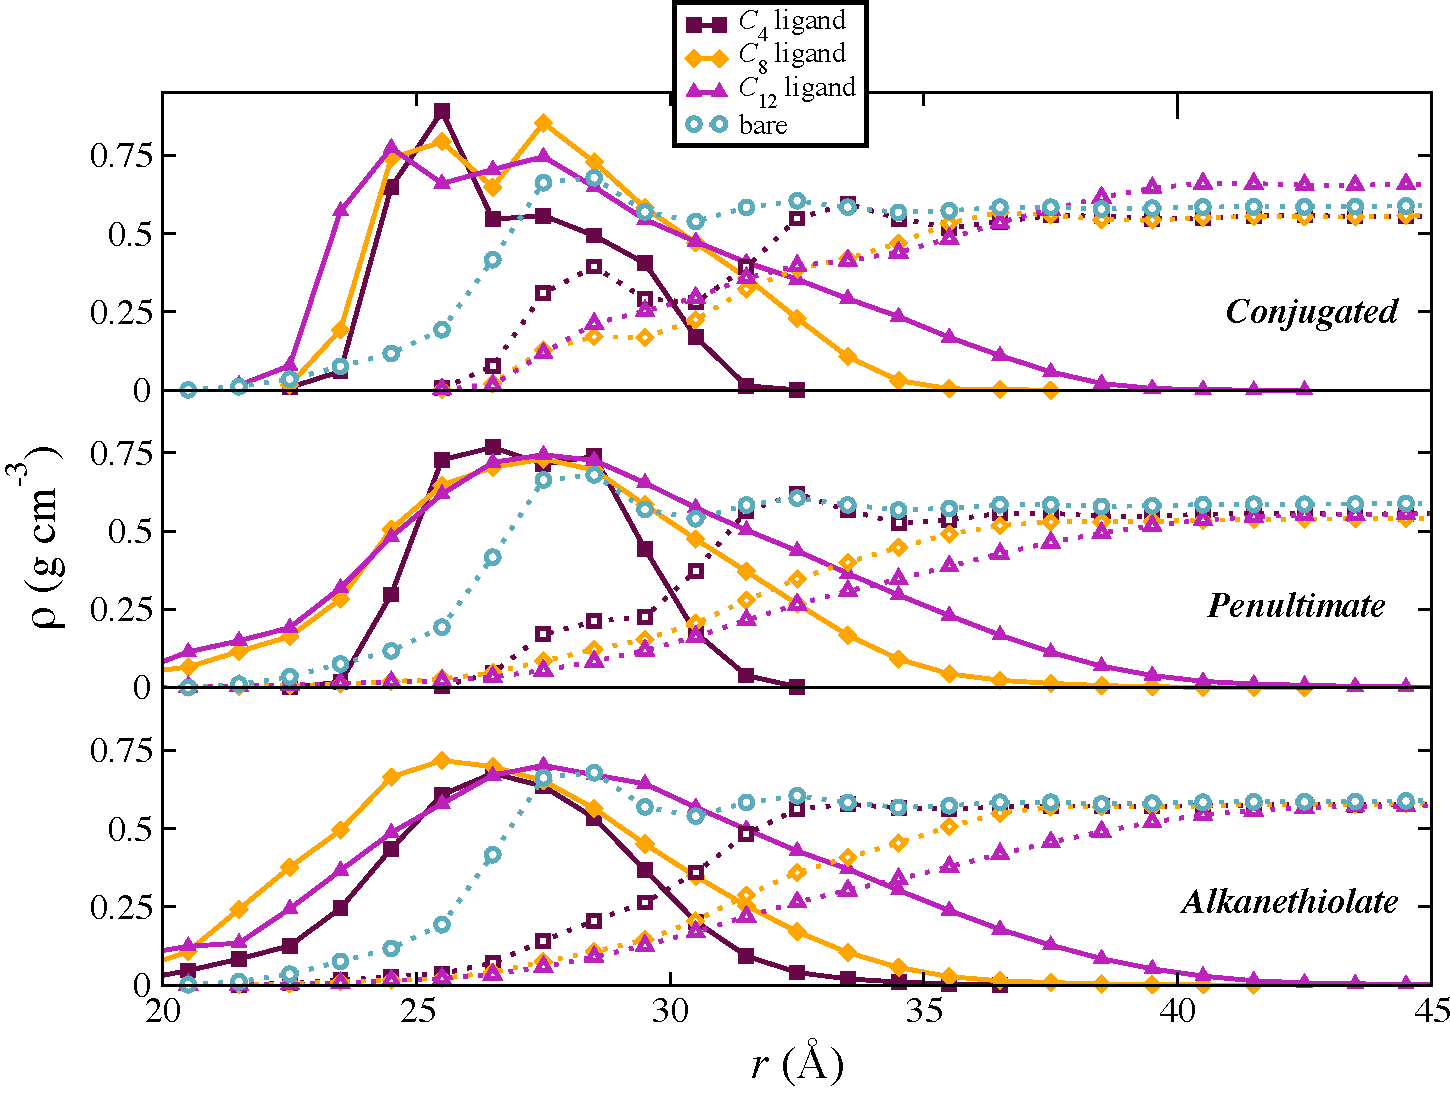
\includegraphics[width=\linewidth]{figures/density}
  \caption{Radial density profiles for 25 \AA\ radius nanoparticles
    with no ligands (circles), C$_{4}$ ligands (squares), C$_{8}$
    ligands (diamonds), and C$_{12}$ ligands (triangles). Ligand
    density is indicated with filled symbols, solvent (hexane) density
    is indicated with open symbols. As ligand chain length increases,
    the nearby solvent is excluded from the ligand layer.  The
    conjugated ligands (upper panel) can create a separated solvent
    shell within the ligand layer and also allow significantly more
    solvent to penetrate close to the particle.}
  \label{fig:density}
\end{figure}

The differences between the radii at which the hexane surrounding the
ligand-covered particles reaches bulk density correspond nearly
exactly to the differences between the lengths of the ligand
chains. Beyond the edge of the ligand layer, the solvent reaches its
bulk density within a few angstroms. The differing shapes of the
density curves indicate that the solvent is increasingly excluded from
the ligand layer as the chain length increases.

The conjugated ligands create a distinct solvent shell within the
ligand layer and also allow significantly more solvent to penetrate
close to the particle. A density overlap parameter can be defined,
\begin{equation}
O_{l-s} = \frac{1}{V} \int_0^{r_\mathrm{max}} 4 \pi r^2 \frac{4 \rho_l(r) \rho_s(r)}{\left(\rho_l(r) +
    \rho_s(r)\right)^2} dr
\end{equation}
where $\rho_l(r)$ and $\rho_s(r)$ are the ligand and solvent densities
at a radius $r$, and $V$ is the total integration volume
($V = 4\pi r_\mathrm{max}^3 / 3$).  The fraction in the integrand is a
dimensionless quantity that is unity when ligand and solvent densities
are identical at radius $r$, but falls to zero when either of the two
components are excluded from that region.

\begin{figure}
  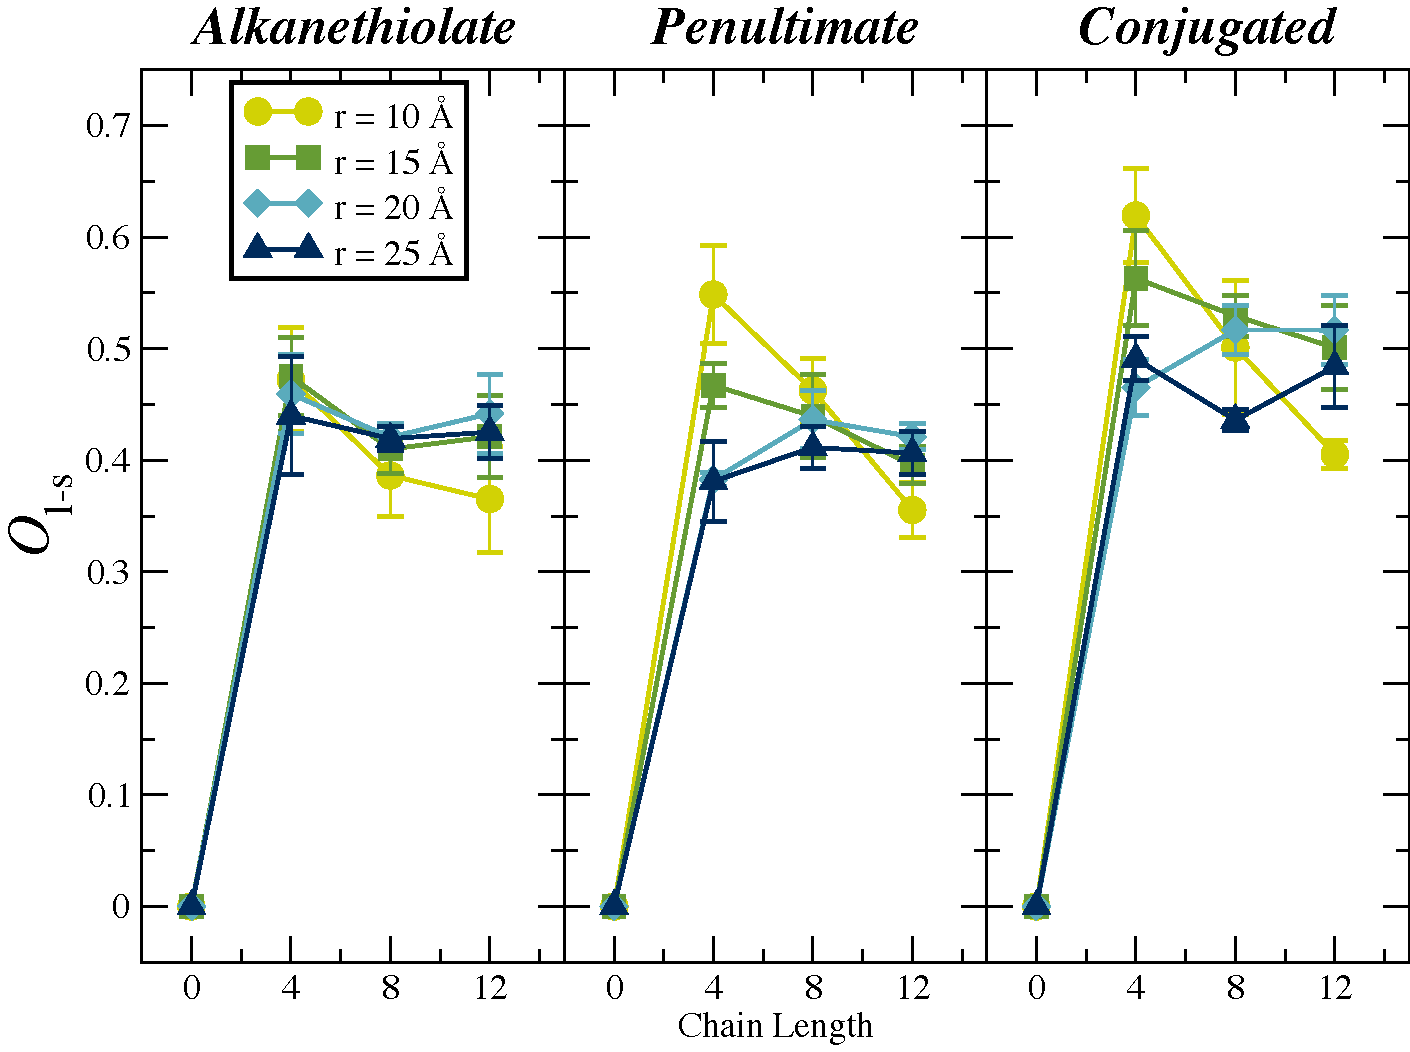
\includegraphics[width=\linewidth]{figures/rho3}
  \caption{Density overlap parameters ($O_{l-s}$) for solvated
    nanoparticles protected by thiolate ligands. In general, the
    rigidity of the fully-conjugated ligands provides the easiest
    route for solvent to enter the interfacial region. Additionally,
    shorter chains allow a greater degree of solvent penetration of
    the ligand layer.}
  \label{fig:rho3}
\end{figure}

The density overlap parameters are shown in Fig. \ref{fig:rho3}.  The
calculated overlap parameters indicate that the conjugated ligand
allows for the most solvent penetration close to the particle, and
that shorter chains generally permit greater solvent penetration in
the interfacial region. Increasing overlap can certainly allow for
enhanced thermal transport, but this is clearly not the only
contributing factor. Even when the solvent and ligand are in close
physical contact, there must also be good vibrational overlap between
the phonon densities of states in the ligand and solvent to transmit
vibrational energy between the two materials.

\subsection{Ligand-mediated Vibrational Overlap}

In phonon scattering models for interfacial thermal
conductance,\cite{Swartz:1989uq,Young:1989xy,Cahill:2003fk,Reddy:2005fk,Schmidt:2010nr}
the frequency-dependent transmission probability
($t_{a \rightarrow b}(\omega)$) predicts phonon transfer between
materials $a$ and $b$.  Many of the models for interfacial phonon
transmission estimate this quantity using the phonon density of states
and group velocity, and make use of a Debye model for the density of
states in the solid.

A consensus picture is that in order to transfer the energy carried by
an incoming phonon of frequency $\omega$ on the $a$ side, the phonon
density of states on the $b$ side must have a phonon of the same
frequency. The overlap of the phonon densities of states, particularly
at low frequencies, therefore contributes to the transfer of heat.
Phonon scattering must be done in a direction perpendicular to
the interface.  In the geometries described here, there are two
interfaces (particle $\rightarrow$ ligand, and ligand $\rightarrow$
solvent), and the vibrational overlap between the ligand and the other
two components is relevant to heat transfer.
 
To estimate the relevant densities of states, I have projected the
velocity of each atom $i$ in the region of the interface onto a
direction normal to the interface. For the nanosphere geometries
studied here, the normal direction depends on the instantaneous
positon of the atom relative to the center of mass of the particle.
\begin{equation}
v_\perp(t) = \mathbf{v}(t) \cdot \frac{\mathbf{r}(t)}{\left|\mathbf{r}(t)\right|}
\end{equation}
The quantity $v_\perp(t)$ measures the instantaneous velocity of an
atom in a direction perpendicular to the nanoparticle interface.  In
the interfacial region, the autocorrelation function of these
velocities,
\begin{equation}
  C_\perp(t) = \left< v_\perp(t) \cdot v_\perp(0) \right>,
\end{equation}
will include contributions from all of the phonon modes present at the
interface.  The Fourier transform of the time-symmetrized
autocorrelation function provides an estimate of the vibrational
density of states,\cite{Shin:2010sf}
\begin{equation}
  \rho(\omega) = \frac{1}{\tau} \int_{-\tau/2}^{\tau/2} C_\perp(t) e^{-i
    \omega t} dt.
\end{equation}
Here $\tau$ is the total observation time for the autocorrelation
function.  In Fig.~\ref{fig:vdos} shows the low-frequency region of
the normalized vibrational densities of states for the three chemical
components (gold nanoparticle, C$_{12}$ ligands, and interfacial
solvent).  The double bond in the penultimate location is a small
perturbation on ligands of this size, and that is reflected in
relatively similar spectra in the lower panels.  The fully conjugated
ligand, however, shifts the peak in the lowest frequency band from
$\sim 29 \mathrm{cm}^{-1}$ to $\sim 55 \mathrm{cm}^{-1}$, yielding
significant overlap with the density of states in the nanoparticle.
This ligand increases the overlap with the solvent density of
states in a band between 280 and 380 $\mathrm{cm}^{-1}$.  This
provides some physical basis for the high interfacial conductance
observed for the fully conjugated $C_8$ and $C_{12}$ ligands.

\begin{figure}
  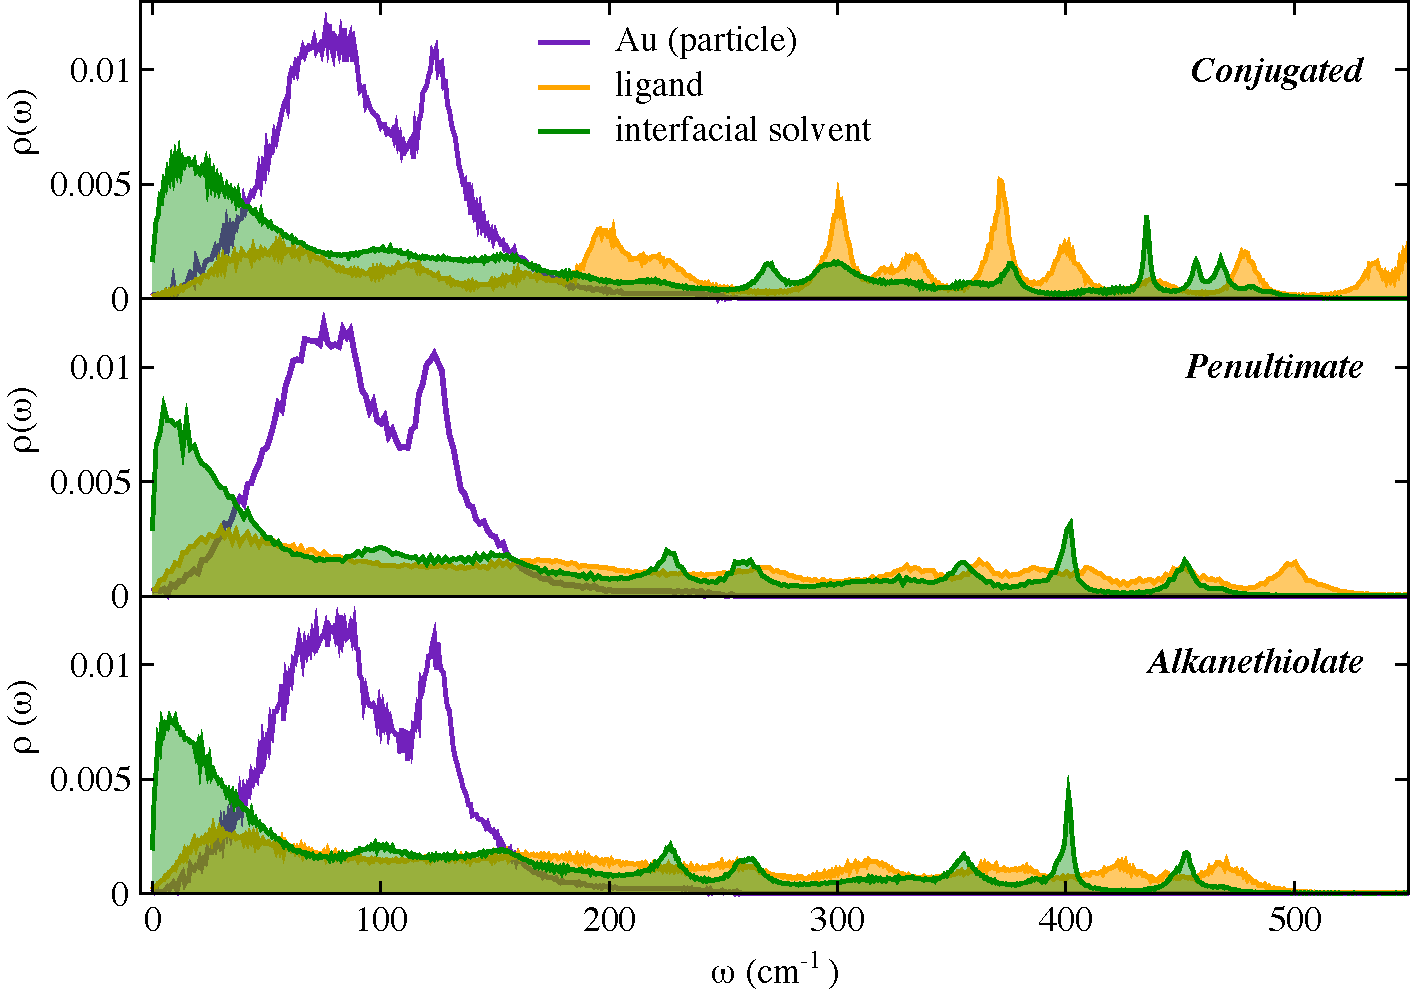
\includegraphics[width=\linewidth]{figures/rho_omega_12}
  \caption{The low frequency portion of the vibrational density of
    states for three chemical components (gold nanoparticles, C$_{12}$
    ligands, and hexane solvent). These densities of states were
    computed using the velocity autocorrelation functions for atoms in
    the interfacial region, constructed with velocities projected onto
    a direction normal to the interface.}
  \label{fig:vdos}
\end{figure}

The similarity between the density of states for the alkanethiolate
and penultimate ligands explains why the interfacial
conductance is nearly the same for these two ligands, particularly at
longer chain lengths.

%%%%%%%%%%%%%%%%%%%%%%%%%%%%%%%%%%%%%%%%%%%%%%%%%%%%%%%%%%%%%%%%%%%%%%%%%%%%%%%%%%%
%		DISCUSSION
%%%%%%%%%%%%%%%%%%%%%%%%%%%%%%%%%%%%%%%%%%%%%%%%%%%%%%%%%%%%%%%%%%%%%%%%%%%%%%%%%%%
\section{Discussion}

The chemical bond between the metal and the ligand introduces
vibrational overlap that is not present between the bare metal surface
and solvent. Thus, regardless of ligand identity or chain length, the
presence of a half-monolayer ligand coverage yields a higher
interfacial thermal conductance value than the bare nanoparticle.  The
mechanism for the varying conductance for the different ligands is
somewhat less clear.  Ligand-based alterations to vibrational density
of states is a major contributor, but some of the ligands can disrupt
the crystalline structure of the smaller nanospheres, while others can
re-order the interfacial solvent and alter the interpenetration
profile between ligand and solvent chains. Further work to separate
the effects of ligand-solvent interpenetration and surface
reconstruction is clearly needed for a complete picture of the heat
transport in these systems.

%%%%%%%%%%%%%%%%%%%%%%%%%%%%%%%%%%%%%%%%%%%%%%%%%%%%%%%%%%%%%%%%%%%%%%%%%%%%%%%
% **ACKNOWLEDGMENTS**
%%%%%%%%%%%%%%%%%%%%%%%%%%%%%%%%%%%%%%%%%%%%%%%%%%%%%%%%%%%%%%%%%%%%%%%%%%%%%%%
%\begin{acknowledgments}
  %Support for this project was provided by the National Science Foundation
  %under grant CHE-1362211. Computational time was provided by the
 % Center for Research Computing (CRC) at the University of Notre Dame.
%\end{acknowledgments}

%\newpage
%\bibliographystyle{aip}
%\bibliography{NPthiols}

%\end{document}


%%%%%%%%%%%%%%%%%%%%%%%%%%%%%%%%%%%%%%%%%%%%%%%%%%%%%%%%%%%%%%%%%%%%%%%%%%%%%%%%%%%
%		CHAPTER 3 -- Morphology Dependence of the Interfacial Thermal Conductance
%%%%%%%%%%%%%%%%%%%%%%%%%%%%%%%%%%%%%%%%%%%%%%%%%%%%%%%%%%%%%%%%%%%%%%%%%%%%%%%%%%%
\chapter{THERMAL TRANSPORT IS INFLUENCE By NANOPARTICLE SHAPE}\label{chap:morph}
%\begin{abstract}
%\section{Abstract}
%  Molecular dynamics simulations were performed to model the
%  interfacial thermal conductance ($G$) from bare gold nanoparticles
%  (icosahedral, cuboctahedral, and spherical) to a hexane
%  solvent. The computed conductance was found to depend not only on
%  particle shape, but also on the size of the nanoparticles,
%  particularly for nanospheres.  These results are compared with
%  conductance out of the planar facets: (111), (100), and (110);
%  all commonly exhibited in small patches by the spherical
%  particles. Undercoordination of the surface atoms and the
%  vibrational density of states in the icosahedra explain some of
%  these observations. The exposed surfaces of icosahedral particles
%  are dominated by (111) facets with 9-coordinated gold atoms.
%  Cuboctahedral particles are dominated by the (100) and (111) facets
%  with 8- and 9-coordinated surface atoms, respectively.  The
%  nanospheres approach a constant surface density of 6-9 coordinated
%  sites at large particle sizes, and these surface atoms play a large
%  role in the conductance to the solvent.  The surface-normal
%  vibrational densities of states were used to explain a simple
%  surface undercoordination model, which shows a size-dependent
%  enhancement of low-frequency coupling to the solvent.
%\end{abstract}


%%%%%%%%%%%%%%%%%%%%%%%%%%%%%%%%%%%%%%%%%%%%%%%%%%%%%%%%%%%%%%%%%%%%%%%%%%%%%%%%%%%
%		INTRODUCTION
%%%%%%%%%%%%%%%%%%%%%%%%%%%%%%%%%%%%%%%%%%%%%%%%%%%%%%%%%%%%%%%%%%%%%%%%%%%%%%%%%%%
\section{Introduction}
Thermal transport between nanoparticles and their surrounding
environments depends on many factors, including particle
size,\cite{Zanjani2014,Liu2015,Wilhelmsen2015,Stocker2016,Tascini2016}
composition,\cite{Wilson:2002uq, Ge:2004yg,Ong:2013rt} surface
modification,\cite{Ge:2004yg,kuang:AuThl,Ong:2013rt,Ong:2014yq,Liu2015,Stocker2016,Hannah2015,Park2016,Meng:2017,Leitner2017}
surface supports,\cite{Schmidt:2010,Park2012} exposed surface
facets,\cite{Norris:2013,Hannah2015,Han:2017} and the chemical details
of the
environment.\cite{Ge2006,Schmidt:2010,Park2012,Ong:2013rt,Ong:2014yq,Wilhelmsen2015,Giri:2016,Park2016,Bhanushali:2017,Yadav:2017}
Particle morphology may also play a role in heat transfer out of
nanostructures.  This is the central question of this work -- all
other things being equal, will different particle morphologies yield
different heat transfer properties to the solvent?

Tascini \textit{et al.}\cite{Tascini2016} studied the
curvature dependence of the interfacial thermal conductance for
partially solvated nanospheres. They found an empirical relationship,
\begin{equation}
G(r) = G(\infty) + \frac{\delta}{r}
\label{Tascini}
\end{equation}
where $G(r)$ is the conductance out of a sphere of radius $r$,
$G(\infty)$ is a parameter describing the infinite-radius limit of the
conductance, and $\delta$ describes the approach to the infinite size
limit. Notably, the Tascini \textit{et al.} simulations predict a
positive $\delta$, where smaller particles exhibit high interfacial
thermal conductance and approach an infinite surface limit that has
lower thermal conductance to the solvent. This makes intuitive sense
-- one might expect the large particle limit to approach the behavior
of flat interfaces.

To test this hypothesis, heat transfer out of gold
nanospheres that were in direct contact with a molecular solvent have been computed. The
spheres were cut out of an infinite FCC lattice and spanned a range of
sizes.  The spheres
expose many surface facets including patches of the (111), (100), and
(110) facets, due to the cuts in the underlying FCC lattice.
The interfacial thermal conductance out of similarly-sized
 icosahedral particles that exhibit only (111) facets and cuboctahedral particles that display
only (111) and (100) facets have been compared to the spheres. 
Additionally, the interfacial thermal conductance to flat interfaces 
that match the facets exposed on the surfaces of the spheres are presented
for comparison.

One possible explanation for an empirical relationship like
Eq. (\ref{Tascini}) is that there is a significant contribution to
interfacial thermal conductance that depends on the surface area to
volume ratio, suggesting a large role for the surface atoms. In 
previous work, the thermal conductance out of chemically-modified gold
surfaces was examined via reverse nonequilibrium molecular dynamics
(RNEMD). \cite{kuang:AuThl,Stocker:2014qq,Stocker2016} %add citation
In these studies, surfactants attached to the gold surfaces contained
a strong gold -- sulfur interaction that acted as a bridge for
vibrational energy to travel to the ligand.  Although the presence and
density of the ligand layer has a large effect on the interfacial
conductance, no clear trend was established regarding the size and
curvature of the underlying nanoparticles. Previous studies from
Tascini \textit{et al.}\cite{Tascini2016} and Ong \textit{et
  al.}\cite{Ong:2014yq} predict a decrease in the interfacial thermal
conductance as the particle radius increases, although Ong \textit{et
  al.}\cite{Ong:2014yq} and Zanjani \textit{et al.}\cite{Zanjani2014}
predict higher thermal conductivity with increasing core diameter in
nanocrystal arrays. However, if surface modifications dominate
conductance, the presence of a moderate density of ligands will
obscure the effects of particle curvature.

\subsection{Size- and temperature-dependent particle morphologies}
The nanoparticles simulated for this work ranged in size from 309
atoms to 14,993 atoms.  Ercolessi \textit{et al.}\cite{Ercolessi1991}
annealed at temperatures from 400K to 1400K and found the dominant
structures for different sizes of gold particles
($N = 100 \text{-} 900$ atoms).  For $N = 100 \text{-} 200$, the
structures were dominated by glassy clusters while for
$N = 200 \text{-} 900$, the structures were predominantly
cuboctahedral. Similarly, Myshlyavtsev and Stishenko found, when
comparing gold nanostructures, a transition from a fully (111)
icosahedral structure to a (100)-terminated cuboctahedral structures
between 561 to 1,415 atoms, depending on the potential energy
function.\cite{Myshlyavtsev2013} Distinct vibrational densities of
states have also been observed for the cuboctahedral clusters relative
to icosahedra.\cite{Sauceda2015}

In a study of the thermal stability of gold icosahedra, Wang
\textit{et al.}\cite{Wang2004} found that softening of the vertex and
edge atoms occurs at $\approx$ 800K.  During this process they saw
enhanced surface atom diffusion due to the mobility of the vertex and
edge atoms.

The size range ($N = 300 \text{-} 15,000$) and temperatures (250K) for
the calculations described here exhibit stable icosahedra with
relatively low surface atom mobility, except for the smallest
($r = 18 \text{-} 22$~\AA) particles, which may be metastable relative to
cuboctahedra.

\subsection{Theory}
Under the diffuse mismatch model (DMM), the thermal conductance at an interface between $a$ and $b$ can be approximated,  
\begin{equation}
G_{ab} = \frac{1}{4 \pi} \sum_p \int_\omega \int_\theta \int_\phi \hbar \omega \frac{\partial f}{\partial T}  v_a  \rho_a  \tau_{ab} \cos\theta \sin\theta d\theta d\phi d\omega
\end{equation}
where $f$ is the Bose-Einstein distribution function, $v_a(\omega, p)$
is the group velocity (on side $a$) for a phonon characterized by
frequency $\omega$, moving in direction ($\theta, \phi$) with
polarization $p$.  The relevant material properties are the density of
phonon states, $\rho_a(\omega, p)$ and the transmission probability,
$\tau_{ab}(\omega, p)$, at the
interface.\cite{Swartz:1989uq,Reddy:2005fk,Monachon2016}
%The DMM also assumes that phonons scatter into states with the same frequency on either side, and that the scattering phonons lose memory of their incident angles.  This requires a symmetry in the transmission probabilities,
% \begin{equation}
% \tau_{ab}(\omega) = 1 - \tau_{ba}(\omega)
% \end{equation}

The diffuse mismatch model has a number of significant issues,
particularly when the Debye model is a poor representation of the
density of states, or where there is a fictitious boundary between
identical materials (where the DMM predicts a non-zero
resistance).\cite{Monachon2016} There is also an assumption of
detailed balance built-in to the model,\cite{Chen2005} which requires
the two sides to be at equilibrium.  This assumption is violated under
non-equilibrium conditions, as in the RNEMD simulations used
here. Although the DMM is not quantitative, it does suggest a role for
frequency-dependent phonon transmission at the interface and 
that isolating the frequencies of the phonons moving
towards the interface could aid in understanding interfacial
conductance. 

Using atomic velocities projected in a direction normal to the
interface,
\begin{equation}
v^{\perp}_i(t) = \mathbf{v}_i(t) \cdot \hat{\mathbf{n}}, 
\end{equation}
it is straightforward to compute vibrational power spectra,
\begin{equation}
  \rho^\perp (\omega) = \frac{1}{\tau} \int_{-\tau/2}^{\tau/2} \langle v^{\perp}(t) \cdot v^{\perp}(0) \rangle e^{-i\omega t} dt
\label{eq:DOS}
\end{equation}
which have been averaged over direction and polarization, where $\tau$
is the total observation time for the autocorrelation function.  
This can be used to approximate the density of phonon states of the two
materials near the interface, which can provide a clearer picture of
vibrational communication between the two materials. 
%We can also use information about the \textit{locations} of the vibrating atoms to arrive at a transmission model that gives a clearer picture of vibrational communication across the interface.
By further restricting the density of states calculation to specific
atoms at the metallic side of the interface, it might to provide a
mechanism for heat flow from the solid and into the surrounding
liquid.

To compute interfacial thermal conductance values directly,
reverse non-equilibrium molecular dynamics (RNEMD)
simulations are utilized.\cite{Muller-Plathe:1997wq,Kuang:2012fe} RNEMD imposes an
unphysical kinetic energy exchange between the center of the particle
and a spherical shell of solvent that is well-separated from the
interface.  The system responds by creating a thermal gradient in the
metal and solvent regions, and a temperature discontinuity at the
interface between the particle and the solvent. The Kapitza resistance
of the interface,
\begin{equation}
  R_\mathrm{K} = \frac{1}{G} = \frac{1}{q_r} \sum_i \left(T_{i+i} - T_i\right) 4 \pi r_i^2,
  \label{sphericalG}
\end{equation}
is estimated by summing the individual thermal resistances of
concentric spherical shells as the radius
increases.\cite{Stocker:2014qq} Here, $T_i$ is the temperature of a
shell with radius $r_i$, and $q_r$ is the heat rate (the relevant
measure of thermal transport in spherical geometries). The heat rate
is the surface area of the particle times that of the imposed
flux. The interfacial thermal conductance of the interface, $G$ is the
inverse of the net Kapitza resistance.  For interfaces of appreciable
width, the relevant shells for measuring interfacial resistance are
the largest shell that is unambiguously in the particle and the
smallest shell that is unambiguously in the solvent.

For planar or periodic geometries, the interfacial thermal conductance
can be similarly computed by imposing a non-physical flux between two
separated slabs in the simulation cell. In this case, the Kapitza
resistance,
\begin{equation}
  R_\mathrm{K} = \frac{1}{G} = \frac{\Delta T}{J_z},
\label{planarG}
\end{equation}
depends on the imposed kinetic energy flux, $J_z$, in a direction
normal to the interface ($z$), and the steady-state temperature drop,
$\Delta T$, across the interface.\cite{Kuang:2012fe}

%%%%%%%%%%%%%%%%%%%%%%%%%%%%%%%%%%%%%%%%%%%%%%%%%%%%%%%%%%%%%%%%

\section{Computational Details}

Solvated gold nanoparticles ranging in diameter from 20-80 \AA\ were
simulated using reverse non-equilibrium molecular dynamics (RNEMD) in
a spherical shell of hexane. Similar planar systems, displaying (111),
(110), and (100) facets with hexane solvent were also prepared.  The
following sections describe the system composition, 
the potentials used to calculate the
interactions in the system, as well as the simulation protocol.

\subsection{System Composition}
Both the nanoparticle and planar systems contain only gold atoms and
hexane molecules.  The composition of the planar systems can be found
in Table \ref{tab:facet} and the nanoparticle system details can be
found in Tables \ref{tab:spheres}, \ref{tab:icosahedra}, and \ref{tab:cubos}.

\begin{table}
\centering
\caption{Composition of the solvated planar facet systems and the
  physical extent of the gold slabs ($L_x$, $L_y$, and $L_z$). The
  hexane molecules occupy the remainder of a 100 \AA\ box (length
  measured along the $z$-axis).
  \label{tab:facet}}
\begin{tabular}{ c|cccc| c }
\toprule
Facet & Au atoms & $L_x$ (\AA) &$L_y$ (\AA) & $L_z$ (\AA) & Hexane Molecules\\
\midrule
(111) &  972 & 25.915   & 29.888 & 18.952 & 284      \\
(110) & 1800 & 40.131   & 34.089 & 20.280 & 498      \\
(100) & 1008 & 24.322   & 24.382 & 26.422 & 200      \\
\bottomrule
\end{tabular}
\end{table}

\begin{table}
\centering
\caption{Composition of the solvated nanosphere simulations.
  \label{tab:spheres}}
\begin{tabular}{ c|cc }
\toprule
        & \multicolumn{2}{c}{Components}\\
Particle Radius (\AA) & Au atoms & Hexane Molecules \\
\midrule
 9.20 $\pm$ 0.28  & 249   &  2894      \\
14.30 $\pm$ 0.31  & 887   &  6304      \\
19.07 $\pm$ 0.28  & 1985  &  8555      \\
24.09 $\pm$ 0.32  & 3925  & 11576      \\
29.03 $\pm$ 0.29  & 6699  & 15376      \\
34.01 $\pm$ 0.32  & 10641 &  9235      \\
38.88 $\pm$ 0.31  & 15707 &  8056      \\
\bottomrule
\end{tabular}
\end{table}

\begin{table}
\centering
\caption{Composition of the solvated icosahedral nanoparticle simulations.
  \label{tab:icosahedra}}
\begin{tabular}{ cc|cc }
\toprule
       &            & \multicolumn{2}{c}{Components}\\
$n$ shells & radius (\AA) & Au atoms & Hexane Molecules \\
\midrule
4  &  9.45 $\pm$ 0.15  &   309 &  2894      \\
5  & 11.75 $\pm$ 0.17  &   561 &  4320      \\
6  & 14.07 $\pm$ 0.19  &   923 &  6304      \\
7  & 16.39 $\pm$ 0.21  &  1415 &  7414      \\
8  & 18.71 $\pm$ 0.25  &  2057 &  8555      \\
9  & 21.04 $\pm$ 0.27  &  2869 &  8555      \\
10 & 23.36 $\pm$ 0.30  &  3871 & 11576      \\
11 & 25.69 $\pm$ 0.32  &  5083 & 11576      \\
12 & 28.02 $\pm$ 0.35  &  6525 & 11576      \\
13 & 30.35 $\pm$ 0.38  &  8217 &  7741      \\
14 & 32.67 $\pm$ 0.41  & 10178 &  9235      \\
15 & 35.00 $\pm$ 0.43  & 12430 & 10911      \\
16 & 37.33 $\pm$ 0.66  & 14993 & 11576      \\
\bottomrule
\end{tabular}
\end{table}

\begin{table}
\centering
\caption{Composition of the solvated cuboctahedral nanoparticle simulations.
  \label{tab:cubos}}
\begin{tabular}{ c|cc }
\toprule
        & \multicolumn{2}{c}{Components}\\
 radius(\AA)      & Au atoms & Hexane Molecules \\
\midrule
 7.41 $\pm$ 0.35  &   147 & 11360      \\
10.16 $\pm$ 0.53  &   309 &  3387      \\
12.15 $\pm$ 0.50  &   561 &  5888      \\
14.98 $\pm$ 0.69  &   923 &  7414      \\
16.93 $\pm$ 0.65  &  1415 &  9440      \\
19.80 $\pm$ 0.85  &  2057 &  9380      \\
21.73 $\pm$ 0.82  &  2869 & 10317      \\
24.13 $\pm$ 0.90  &  3871 & 14185      \\
26.53 $\pm$ 0.99  &  5083 & 19585      \\
31.34 $\pm$ 1.15  &  8217 & 12626      \\
36.15 $\pm$ 1.32  & 12431 & 17457     \\
\bottomrule
\end{tabular}
\end{table}

Planar systems were constructed with the exposed $(hkl)$ facets
directed normal to the positive and negative $z$-axis.  The simulation
cell dimensions were set by the facet, and the simulation box was
enlarged along the $z$ dimension to a fixed size of 100 \AA.  The
remaining space was filled with hexane molecules to a density of
0.6548 $\text{g cm}^{-3}$.


%%%%%%%%%%%%%%%%%%%%%%%%%%%%%%%%%%%%%%%%%%%%%%%%%%%%%%%%%%%%%%%%%%%%%%%%%%%%%%%%%%%
%		FORCE FIELDS
%%%%%%%%%%%%%%%%%%%%%%%%%%%%%%%%%%%%%%%%%%%%%%%%%%%%%%%%%%%%%%%%%%%%%%%%%%%%%%%%%%%
\subsection{Force Fields}

For this work, gold -- gold interactions are calculated using the
quantum Sutton-Chen (QSC) model.\cite{Qi:1999ph} The hexane solvent is
described by the TraPPE united atom (UA)
model.\cite{TraPPE-UA.alkanes} The bonds in TraPPE-UA are rigid, but
here the bonds are made flexible using harmonic force constants
borrowed from OPLS-AA for intra-molecular sites closer than 3
bonds.\cite{Jorgensen98a} The interactions between Au atoms and atoms
on the hexane molecules were fit to a pairwise Lennard-Jones
potentials based on a study by Hautman and Klein for Au(111)
surfaces.\cite{hautman:4994} Details of the interaction potentials are
identical to previous work and previous chapter on heat 
transport for thiolate-protected gold nanospheres.\cite{Stocker2016}

%%%%%%%%%%%%%%%%%%%%%%%%%%%%%%%%%%%%%%%%%%%%%%%%%%%%%%%%%%%%%%%%%%%%%%%%%%%%%%%%%%%
%		SIMULATION PROTOCOL
%%%%%%%%%%%%%%%%%%%%%%%%%%%%%%%%%%%%%%%%%%%%%%%%%%%%%%%%%%%%%%%%%%%%%%%%%%%%%%%%%%%
\subsection{Simulation Protocol}
The gold nanospheres were prepared by cutting a FCC lattice with radii ranging
10 - 40 \AA. 
Icosahedral particles were
constructed in nested shell structures, built around an ideal
icosahedral core.  Cuboctahedral particles were built by cutting (111)
and (100) facets from a FCC lattice.
All particles were thermally equilibrated before being
solvated with thermally equilibrated hexane using packmol.\cite{packmol}
Once solvated, the systems were equilibrated for a minimum of 1 ns 
using the Langevin Hull 
integrator with an external bath characterized by 50 atm of
pressure and a temperature bath at 250K.\cite{Vardeman2011}
Random seeds were used in both the packing of the solvent and the equilibration process to ensure independent samples.

Planar interfaces displaying the Au(111), Au(110), and Au(100) facets
were prepared as slabs $\sim$ 20 \AA\ thick with the relevant facets
rotated normal to the $z$-axis. Surface stress was removed by relaxing
the systems for 1 ns at 250 K in a constant surface tension
(N\(\gamma\)T) ensemble with zero applied surface tension, followed by
1 ns in the microcanonical (NVE) ensemble.  Hexane molecules were
packed into the remaining box volume with a density of 0.6548
g/cm$^3$. The solvated systems were then equilibrated using the
canonical (NVT) ensemble at 250 K for 1 ns followed by further
relaxation in the microcanonical ensemble for 1 ns.

Following equilibration, the relevant thermal flux was applied for 1
ns for the nanoparticle systems and 3 ns for the planar systems,
allowing for a steady-state temperature gradients to develop. Mean
temperatures of the system remained at 250K, preserving the solvent
cluster around the nanoparticles and preventing the formation of a
vapor layer. Thermal coupling to the external temperature bath was
removed to avoid interference with the imposed flux. The metal
particles equilibrated rapidly, and were typically found with elevated
temperatures ($\sim$300K) relative to the bulk. Because the solvent
volume is large relative to the particles, the solvent finds a steady
state temperature just below 250K throughout most of the
volume. Adjacent to the surface of the particles, solvent temperatures
are typically close to 260K. The TraPPE-UA hexane model boils at
$\sim$ 330K, so the simulation conditions are reasonable for
maintaining liquid surroundings for the particles.  All simulations
were carried out with the open source molecular dynamics package,
OpenMD.\cite{openmd,OOPSE}

Five separate configurations for each system size were simulated to
provide statistical independence of the hexane packing.  Thermal
conductance was calculated using the same methods found in Stocker
\textit{et al.}\cite{Stocker2016} and in the previous chapter for the non-periodic systems.
Planar systems follow Eq. \ref{planarG}, where the temperature difference across the interface is taken from the outermost gold layer and the first layer of solvent. 

\section{Results and Discussion}
The interfacial thermal conductance ($G$) for hexane-solvated
spherical, icosahedral, and cuboctahedral Au nanoparticles was
computed using RNEMD simulations, and was compared with the same
quantity for a series of planar gold interfaces, including the
Au(111), Au(100), and Au(110) interfaces.  These surfaces are all
exhibited as microfacets on the surfaces of the nanospheres, and the
Au(111) facet is the primary facet displayed by the icosahedra,
where the cuboctahedra display Au(111) and Au(100).

Computed interfacial thermal conductance values for the icosahedra,
cuboctahedra, nanospheres, and flat facets are shown in
Fig. \ref{fig:ico_vs_sphere}.  The nanospheres have a pronounced
dependence on the particle radius, $r$, while the icosahedral
conductance stays relatively close to the value obtained for the
Au(110) facet. Thermal transport out of the cuboctahedral particles
show a mostly linear dependence on particle radius.  The smooth line
going through the conductance values for the spheres is a fit using
the Tascini \textit{et al.}\cite{Tascini2016} model
(Eq. (\ref{Tascini})) with
$G(\infty) = 49.25~\text{MW}~\text{m}^{-2}~\text{K}^{-1}$, and
$\delta = -156.25~\text{MW \AA}~\text{m}^{-2}~\text{K}^{-1}$.
Notably, the simulations presented here project a value for the interfacial
conductance of the infinite spheres that is significantly
\textit{higher} than many of the flat facets.  To explain this
observation, the surface density of undercoordinated atoms
and the vibrational densities of states of these undercoordinated
atoms are discussed in the following sections.

\begin{figure}
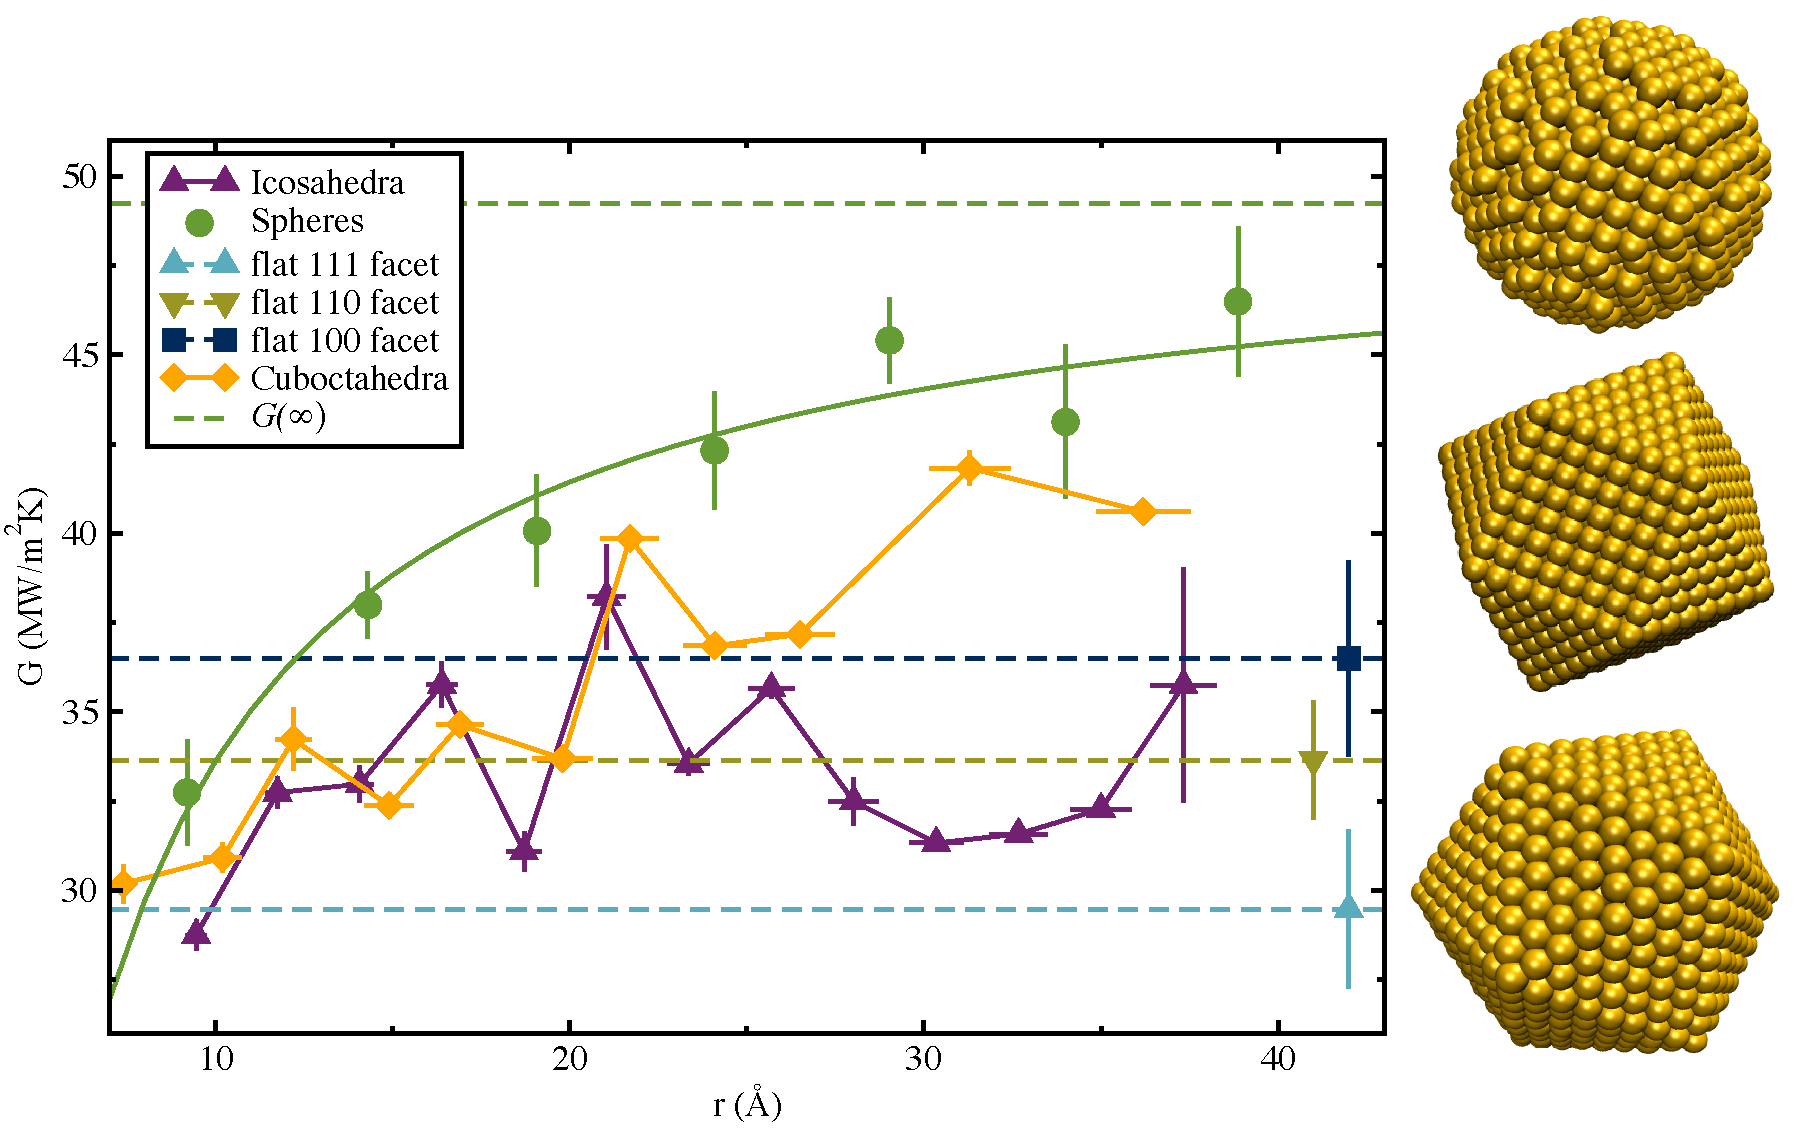
\includegraphics[width=\linewidth]{figures/g-ico-spher-cub.pdf}
	\caption{Interfacial thermal conductance, $G$, for bare gold
          nanospheres, cuboctahedra, and icosahedra in contact with
          hexane solvent. Conductances for flat Au(111), Au(100), and
          Au(110) interfaces are indicated with dashed horizontal
          lines.  A fit using the model of Tascini \textit{et al.} is
          shown along with the predicted value of $G(\infty)$, the
          infinite particle limit.}
	\label{fig:ico_vs_sphere}
\end{figure}

The spherical particles display all three of the planar facets (as
well as small regions of higher index facets), and for most of the
size range simulated, they also exhibit a significantly higher
interfacial thermal conductance than the low-index facets.

For icosahedral particles, there is no clear dependence of $G$ on the
particle size, and the larger particles exhibit thermal conductance
values slightly above the expected (111) conductance for particles
with $r \approx 35$ \AA. There is some instability in the values of
$G$ in the range of $r = 18-22$ \AA, which is near the 
transition from stable icosahedra to
cuboctahedra.\cite{Myshlyavtsev2013}

\subsection{Hexane Density}
The hexane density as function of distance from the gold at the
interface of the planar facets is provided in Fig. \ref{fig:dens}. The
solvent in the (111) and (100) systems display similar behavior, while
the solvent near the (110) interface comes closer to the surface
atoms.  In the (110) system, the first layer of hexane is spread out
over a thicker slab in comparison to the other two systems and allows
solvent to come closer to the interfacial atoms.  This is likely due
to the ridges present on this interface.  Within 5 \AA\ of the
interfacial gold layer, the three systems have the same amount of
hexane.

\begin{figure}
        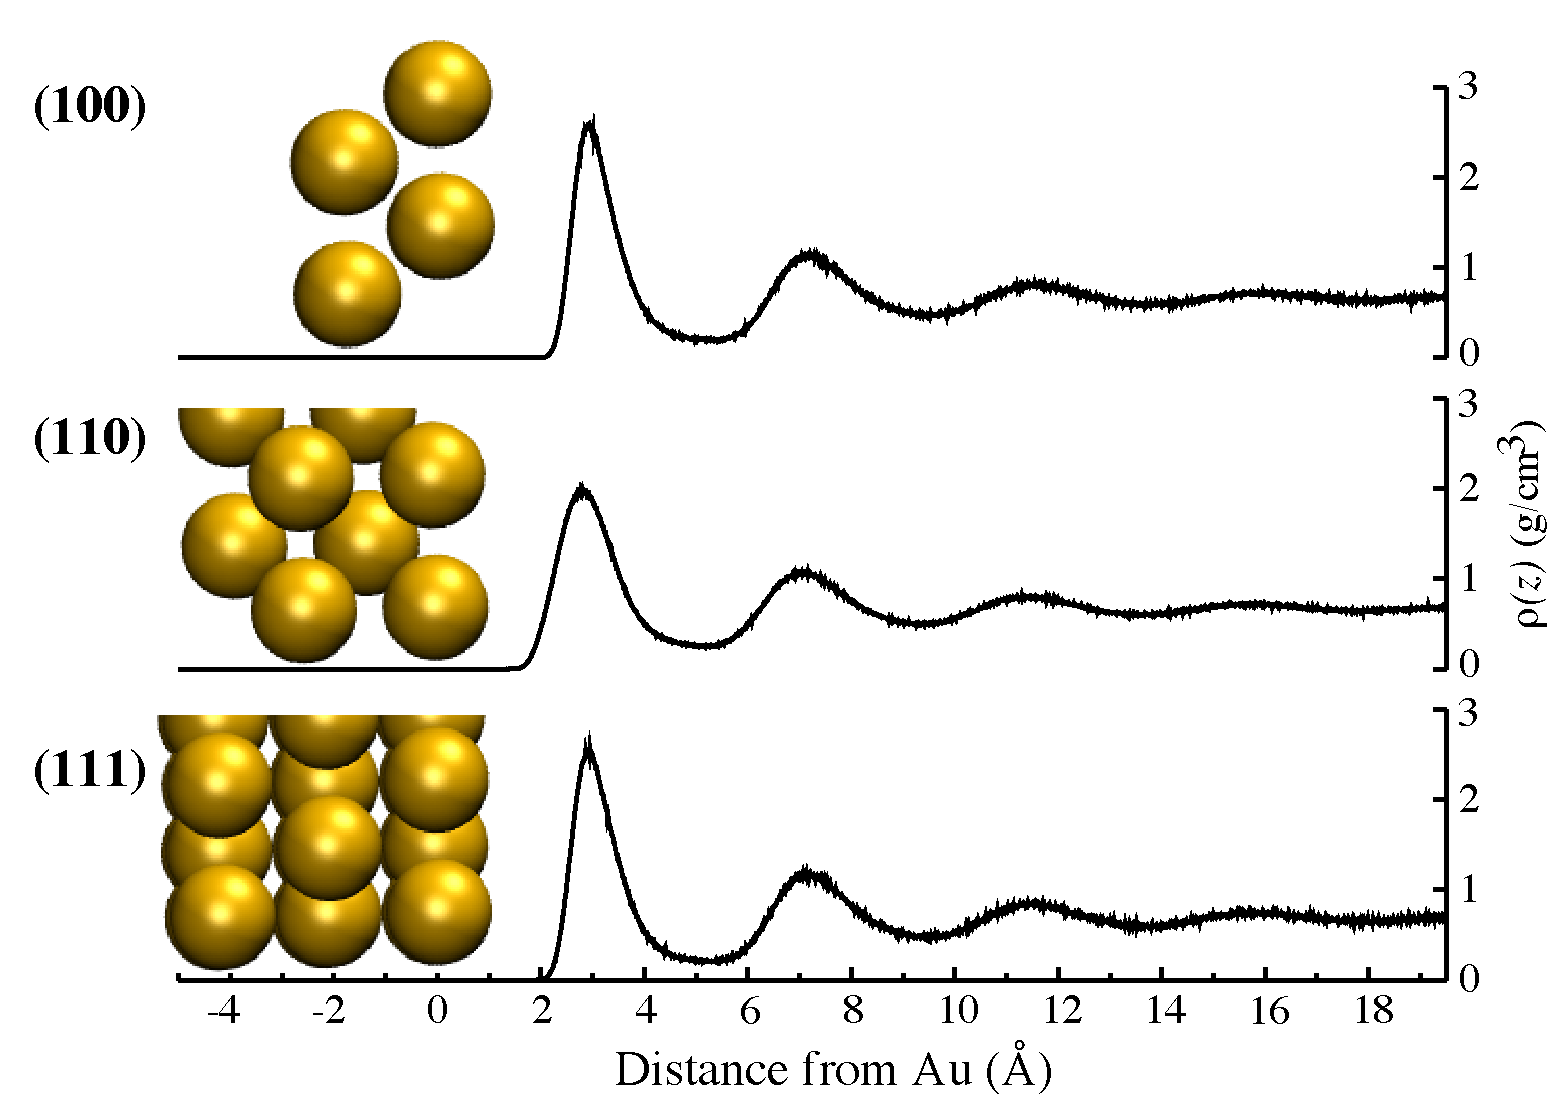
\includegraphics[width=\linewidth]{figures/stacked-hex-facets.pdf}
        \caption{Hexane density as a function of distance from the
          interfacial gold for the (111), (110), and (100) facets. The
          solvent in the (111) and (100) systems display nearly
          identical density profiles. Because the lowest-coordinated
          gold atoms on the (110) facet have a relatively low surface
          density, the hexane molecules are able to get closer to
          these undercoordinated atoms.}
        \label{fig:dens}
\end{figure}

\subsection{Surface Atom Undercoordination}
For the three flat facets, the primary feature that differentiates the
facets is the coordination number (CN) of the atoms that are exposed
to the solvent. In bulk Au, the coordination number of the atoms is
twelve; six neighbors in plane, three below the atom, and three above the
atom. Any atom with a coordination number below twelve would exhibit more
vibrational freedom and is considered an undercoordinated site. The
Au(111) surface presents gold atoms with nine surrounding metallic
atoms ($\text{CN} = 9$) to the solvent, while the Au(100) facet
surface exposes atoms with $\text{CN}=8$.  Au(110) displays a
corrugated surface where the two outer layers of atoms have
$\text{CN}=7$ and $\text{CN}=11$, respectively (displayed in \ref{fig:facets-cn}).
Both of the (110) surface atoms coordination environments
approach the surface close enough to interact with the solvent atoms.

\begin{table}
\centering
\caption{Surface densities $(\text{\AA}^{-2})$ of undercoordinated
  atoms in ideal geometries. $\ell~(\text{\AA})$ is the
  lattice constant of the underlying FCC lattice.  The spheres and
  cuboctahedra are calculated using a gold FCC lattice with $\ell = 4.08
  \text{~\AA}$.  For cuboctahedral particles, the radius ($r$) is computed
  using Eq. \eqref{r_ave}.
  \label{tab:undercoord}}
\begin{tabular}{ c|cccc }
\toprule
\multirow{2}{*}{surface} & \multicolumn{4}{c}{Coordination Number}\\
        & 6 & 7 & 8 & 9 \\
 \midrule
(111)      & 0 & 0     & 0     & $\frac{4 \sqrt{3}}{3 \ell^2}$ \\
(100)      & 0 & 0     & $\frac{2}{\ell^2}$ & 0     \\
(110)      & 0 & $\frac{\sqrt{2}}{\ell^2}$ & 0     & 0     \\
 \midrule
Spheres (large $r$ limit)    & 0.021 & 0.025 & 0.021 & 0.032\\ \\
Icosahedra ($n$ shells)  & $\frac{8\sqrt{3}}{5\ell^2n^2}$  &  0 &
 $\frac{4\sqrt{3}(n-1)}{\ell^2n^2}$ &
 $\frac{4(n - 1)}{\sqrt{3}\ell^2 n}$ \\ \\
Cuboctahedra & 0 & $\frac{1}{r\ell} \left(\frac{3\sqrt{2} + 2\sqrt{6}}{3+\sqrt{3}}\right)$ & $\frac{6}{(3+\sqrt{3})\ell^2}$ & $\frac{4}{(3+\sqrt{3})\ell^2}$\\ \\
\bottomrule
\end{tabular}
\end{table}

In Table \ref{tab:undercoord}, the surface density of
undercoordinated atoms for a set of ideal geometries are provided.
The population
density for the sphere systems in the large radius limit are taken by
averaging the surface densities for ideal gold nanospheres with radii
of 95--100 \AA.  For other FCC-based nanoparticles, it is relatively
simple to convert these surface densities using the lattice constant
of gold, $\ell = 4.08 \text{~\AA}$.

Planar facets have a fixed population density based on the number of
exposed undercoordinated atoms and the physical dimensions of the
exposed facet area in terms of the lattice constant.
\begin{figure}[!htb]
        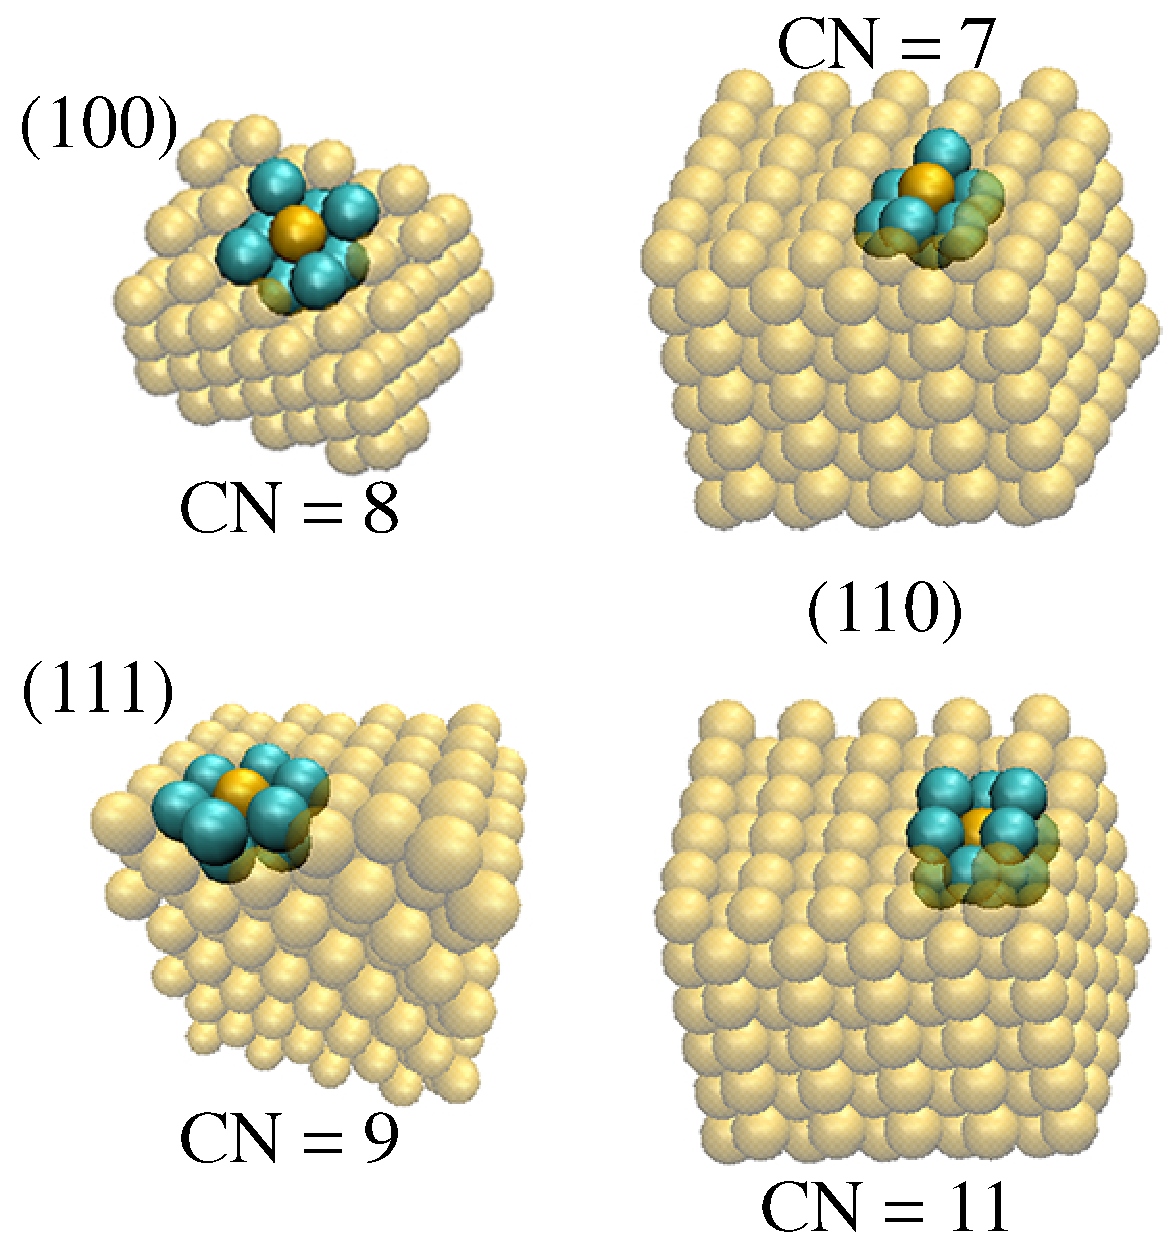
\includegraphics[width=5in]{figures/facets-cn.pdf}
        \caption{Locations of undercoordinated atoms on common gold
          facets. The dark gold atoms indicate atoms of a particular
          coordination number, cyan atoms denote the first nearest
          neighbors of these atoms, and the partially transparent
          lattice illustrates the location of the atoms in the larger
          gold structure. (111) surfaces (lower left) display atoms
          with CN=9, while (100) surfaces (upper left) display atoms
          with CN=8, and (110) surfaces present surface atoms with
          CN=7 and buried atoms with CN=11. }
        \label{fig:facets-cn}
\end{figure}
In an ideal icosahedral nanoparticle with $n$ shells, the surface
population density is computed using the number of vertex, edge, and
face atoms,
\begin{align}
n_\text{vertex} & = 12, \\
n_\text{edge} & = 30 (n -1), \\
n_\text{face} & = 10 n^2 - 30 n + 20.
\end{align}
The number of shells, $n$, is also directly related to the particle
edge length ($a$), radius ($r$), and surface area ($A$) of the
icosahedral particle,
\begin{align}
a & = \ell~n \\
r & = \frac{\ell~n~\sqrt{10+2\sqrt{5}}}{4} \\
A & =  \ell^2~n^2~ 5 \sqrt{3}
\end{align}
where $\ell$ is the lattice constant.

For ideal cuboctahedra, the edge length ($a$) can be used to determine
surface areas for the eight triangular (111) faces and six square
(100) faces,
\begin{align}
A_\mathrm{(111)} &= 2 \sqrt{3} a^2 \\
A_\mathrm{(100)} &= 6 a^2
\end{align}
In addition, cuboctahedra have twenty-four edges (CN = 7, length =
$a$), and twelve vertices (CN = 5).  An approximate radius of the
cuboctahedral particles can be found by averaging the diameter between
parallel square faces and parallel triangular faces,
\begin{equation}
r  = \frac{a}{2} \left(\frac{\sqrt{2}}{2} + \frac{\sqrt{6}}{3}\right)
\label{r_ave}
\end{equation}
Table \ref{tab:undercoord}.  Surface densities of the CN=9 and CN=8
sites are computed using the fraction of total surface area in each of
the (111) and (100) facets, respectively.  For small particles, the
edge atoms (CN=7) can dominate, but for larger particles, the ratio of
CN=8 and CN=9 atoms is constant.



% \begin{figure}
% 	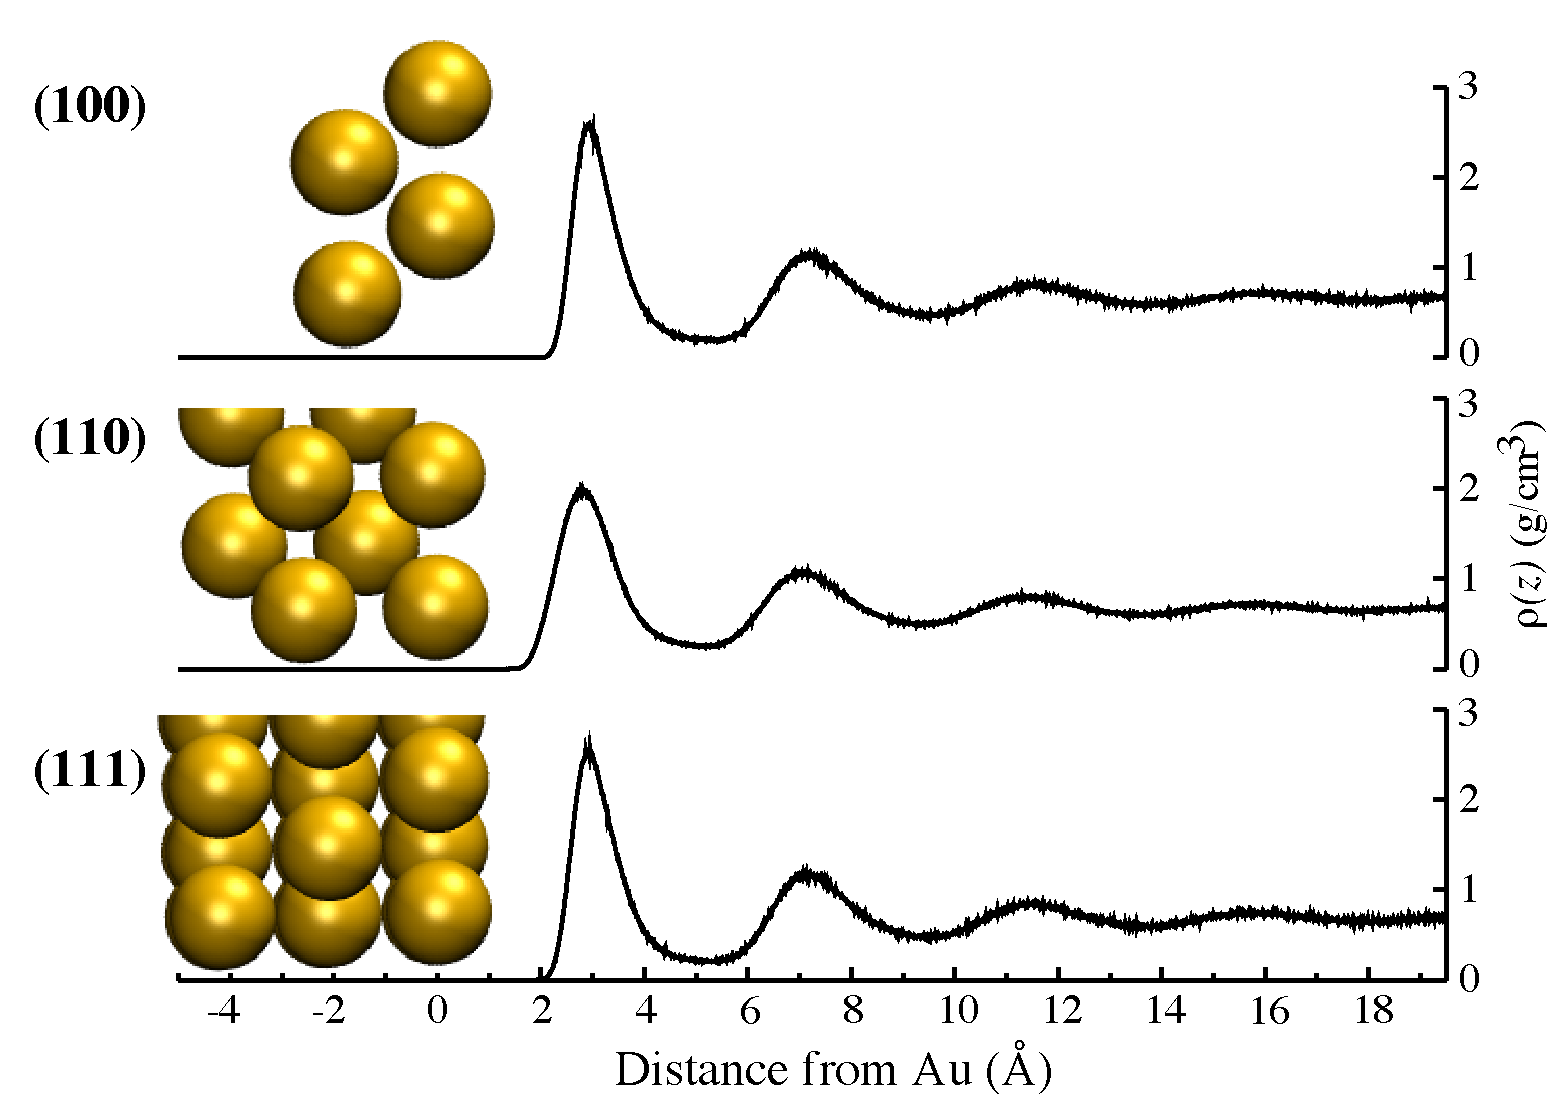
\includegraphics[width=\linewidth]{figures/stacked-hex-facets.pdf}
% 	\caption{The hexane density as a function of distance from the interfacial gold for the (111), (110), and (100) facets. The solvent in the (111) and (100) systems display nearly identical density profiles. Because the lowest-coordinated gold atoms on the (110) facet have a relatively low surface density, the hexane molecules are able to get closer to these undercoordinated atoms.}
% 	\label{fig:dens}
% \end{figure}

Reducing the number of metallic interactions allows the surface atoms
to vibrate at different frequencies than the interior atoms,
populating a portion of the spectrum that overlaps with collective
motions of the solvent molecules. This mechanism may explain the
enhanced interfacial thermal conductance of the (100) facet relative
to the (111) facet. However, it does not explain why the (110) facet
displays an intermediate conductance even though the surface atoms
have a lower coordination number than the (100) facet.  To answer this
question, it is important to consider the surface density of the
undercoordinated atoms as well as the vibrational freedom allowed by
the undercoordination. In Table \ref{tab:au-den} the density
of the solvent-accessible undercoordinated surface atoms for the three
facets is shown. Although the (110) facet displays 7- and 11-coordinated atoms
to the solvent, the $\text{CN}=11$ have vibrational dynamics that are
essentially equivalent to the bulk gold (Fig. \ref{fig:cn-spect}), and the
surface density of these atoms is significantly lower than the surface
density displayed by the (111) and (100) facets.

\begin{figure}[!htb]
  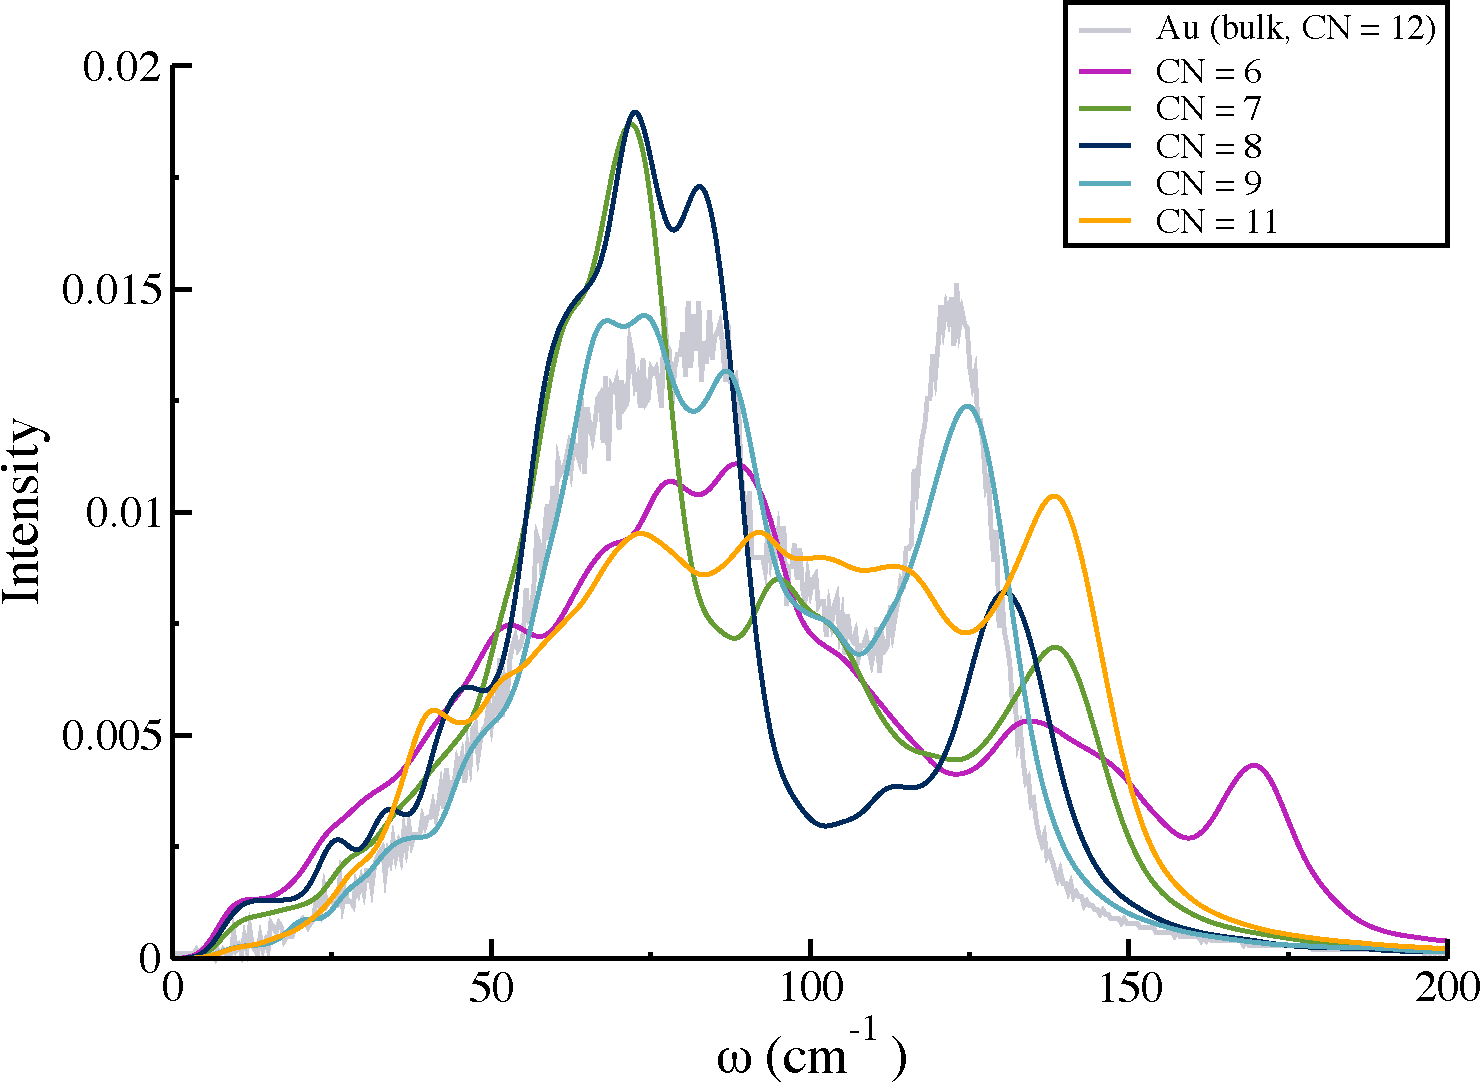
\includegraphics[width=5in]{figures/surface-cn.pdf}
  \caption{The normalized low frequency density of states (DOS) of the
    surface atoms with the coordination number of 6, 7, 8, 9 and 11,
    corresponding to the vertices of the icosahedra, Au(110), Au(100),
    Au(111) and subsurface Au(110), respectively.  Note that CN=11
    atoms near a surface are found adjacent to atoms with lower
    coordination (e.g. CN=7), so the high frequency peak at 138
    cm$^{-1}$ is present for both CN=11 and CN=7.  Low frequency
    contributions at $\sim$ 70 cm$^{-1}$ are enhanced for surface
    atoms with CN=7, 8, and 9.}
  \label{fig:cn-spect}
\end{figure}

\begin{table}[h]
\centering
\caption{The density of undercoordinated gold atoms at the surface of a facet.  
\label{tab:au-den}}
\renewcommand*{\arraystretch}{2}
\begin{tabular}{ ccc }
\toprule
Facet & CN & Surface Density (atoms $\text{\AA}^{-2}$)\\
\midrule
        (111) & 9  & 0.1394 \\
\midrule
        (100) & 8  & 0.1214 \\
\midrule
        (110) & 7  & 0.0877 \\
              & 11 & 0.0877 \\
\bottomrule
\end{tabular}
\end{table}

It is therefore likely that not only the undercoordination of surface
atoms, but also the density of these undercoordinated atoms plays a
role in thermal conductance. In the nanoparticles, surface atoms that
are in physical contact with the solvent have a range of coordination
numbers from $5 - 9$, but only $\text{CN} = 6 - 9$ appear with high
probability.  The surface coordination densities have been calculated
for all of the samples, and the undercoordination density is distinct
for the spheres, icosahedra, and cuboctahedra (See
Fig. \ref{fig:stacked-cn}).

The icosahedral particles display three coordination environments: the
vertices have a $\text{CN} = 6$, while the triangular (111) faces of
the particle have a $\text{CN} = 9$, and the edges connecting the
faces have $\text{CN} = 8$.  As the radius of the icosahedral
particles increases, the surface is dominated by the triangular
facets, so the surface density of the $\text{CN} = 9$ rises.  For
perfect icosahedra, the ideal surface densities are shown as dashed
lines in Fig. \ref{fig:stacked-cn}.

For the simulated systems at 250K, surface vibrational motion leads to
coordination numbers that are lower than one would expect for an ideal
icosahedron. This is evident in the populations of the $\text{CN}= 9$,
which is 20-50\% lower than the ideal case.

\begin{figure}
	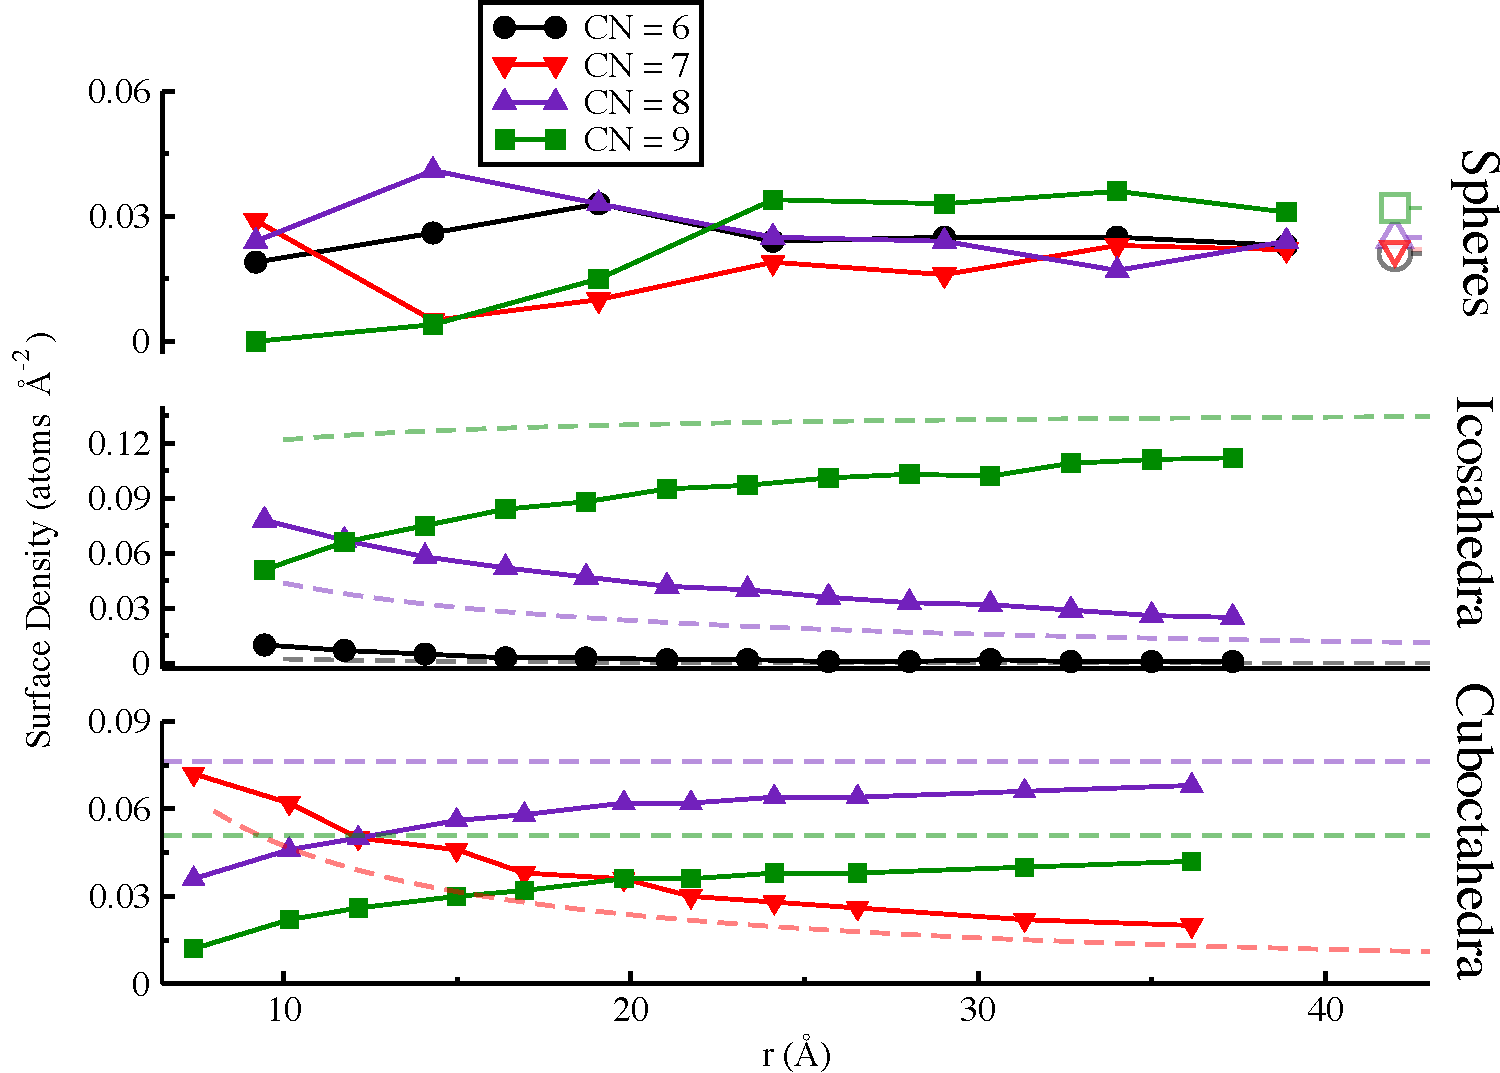
\includegraphics[width=\linewidth]{figures/new-cn.pdf}
	\caption{The coordination number of surface atoms as a
          function of particle size. Filled data points are sampled
          from simulations, while the dashed lines correspond to ideal
          icosahedral and cuboctahedral solids. In the spherical case,
          the large radius limits are shown with open symbols.  The
          large radius limit for the spheres approaches a constant
          density for all undercoordinated sites, while for the
          icosahedra, the 9-coordinated (111) facet dominates. In
          larger cuboctahedra, the relative fraction of 8- and
          9-coordinated surface atoms is largely independent of
          particle size.} 
	\label{fig:stacked-cn}
\end{figure}

In the spherical particles, the surface density of undercoordinated
atoms stabilizes above $r = 25$ \AA.  However, the densities of the
undercoordinated atoms never approach any of the flat facet values (as
is the case in the icosahedra).  The large radius
limit of the spheres are estimated by averaging the surface densities for ideal
spheres of radii 95--100 \AA.  These are shown with open symbols in
the upper panel of Fig. \ref{fig:stacked-cn}.

The cuboctahedral particles approach the ideal solid surface densities
as the radius of the particle increases. Beyond a radius of 15 \AA\,
the cuboctahedra are no longer dominated by edge atoms and flat facets
form the majority of the surface. After this transition the surface
densities quickly stabilize to nearly-ideal cuboctahedral structures.

\subsection{Phonon Spectra}
By selecting specific groups of atoms while computing the vibrational
power spectrum (Eq. \ref{eq:DOS}) the role of
undercoordination on surface vibrational motion can be explored. For thermal
transport, the regions of interest are the nanoparticle atoms in
direct physical contact with the solvent, and those solvent molecules
that form the first solvation shell, i.e. $< 5 \text{\AA}$ from the
gold surface.

Under the QSC potential, the bulk gold vibrational power spectrum
displays two broad peaks, one at $\sim 60-80 \text{~cm}^{-1}$, and
another sharper peak at $\sim 125 \text{~cm}^{-1}$.  The vibrational
densities of states for the four outer layers of the nanoparticles are
shown in Fig. \ref{fig:layer}.  The surface layers for all particles
are dominated by the low frequency portion of the spectrum
($<70 \text{~cm}^{-1}$) and display small morphology-dependent
features at higher frequencies ($140 \text{~cm}^{-1}$). The
low-frequency peak appears at significantly lower frequencies than in
the bulk, and the higher frequency contribution is significantly
broadened.  Spheres and cuboctahedra recover bulk-like densities of
states relatively close to the surface -- only the surface and second
shell are significantly altered from the bulk gold density of
states. In the spheres, the higher frequency contribution
($\sim 150 \text{~cm}^{-1}$) resembles the vibrational density of
states for undercoordinated atoms with CN=8 or 7 (see 
Fig. \ref{fig:cn-spect}).

\subsection{A Brief Aside}
The icosahedra still have perturbed spectra even four layers into the
particles. Icosahedral particles grow around a core with
$\mathrm{I}_h$ symmetry, and the local environment around the atoms
deviates significantly from perfect FCC ordering.  The local bond
orientational order can be described using the method of Steinhardt
\textit{et al.}\cite{Steinhardt1983} 
The local bonding environment,
$\bar{q}_{\ell m}$, for each atom in the system is determined by
averaging over the spherical harmonics between that atom and each of
its neighbors,
\begin{equation}
\bar{q}_{\ell m} = \sum_i Y_\ell^m(\theta_i, \phi_i)
\end{equation}
where $\theta_i$ and $\phi_i$ are the relative angular coordinates of
neighbor $i$ in the laboratory frame.  A global average orientational
bond order parameter, $\bar{Q}_{\ell m}$, is the average over each
$\bar{q}_{\ell m}$ for all atoms in the system. To remove the
dependence on the laboratory coordinate frame, the third order
rotationally invariant combination of $\bar{Q}_{\ell m}$,
$\hat{w}_\ell$, is utilized here.\cite{Steinhardt1983,Vardeman:2008fk}

For $\ell=4$, the ideal face-centered cubic (FCC) local structures
exhibit $\hat{w}_4$ values near -0.159. Because $\hat{w}_4$ exhibits
an extreme value for fcc structures, it is ideal for measuring local
FCC ordering. The spatial distribution of $\hat{w}_4$ local bond
orientational order parameters, $p(\hat{w}_4 , r)$, can provide
information about the location of individual atoms that are central to
local FCC ordering.

The fraction of FCC-ordered gold atoms at a given radius in the
nanoparticle,
\begin{equation}
        f_\mathrm{fcc}(r) = \int_{-\infty}^{w_c} p(\hat{w}_4, r) d \hat{w}_4
\end{equation}
is described by the distribution of the local bond orientational order
parameters, $p(\hat{w}_4, r)$, and $w_c$, a cutoff for the peak
$\hat{w}_4$ value displayed by fcc structures. As seen in previous
chapter,\cite{Stocker2016} $w_c$ value of -0.12 was chosen to isolate the
fcc peak in $\hat{w}_4$.

As shown in Fig. \ref{fig:struct-bowr}, the FCC ordering persists in
the spheres even quite close to the surface, while the icosahedra have
significant populations that deviate from FCC local ordering.  The
cuboctahedra do not have uniform gold population between 30 and 40
\AA, so the fraction of FCC ordering decays starting at 30 \AA.
Although it cannot be concluded that this is the cause of the differences
in the VDOS for the icosahedral particles, it is likely that local
ordering in the metal can alter the bulk densities of states.

\begin{figure}[!htb]
        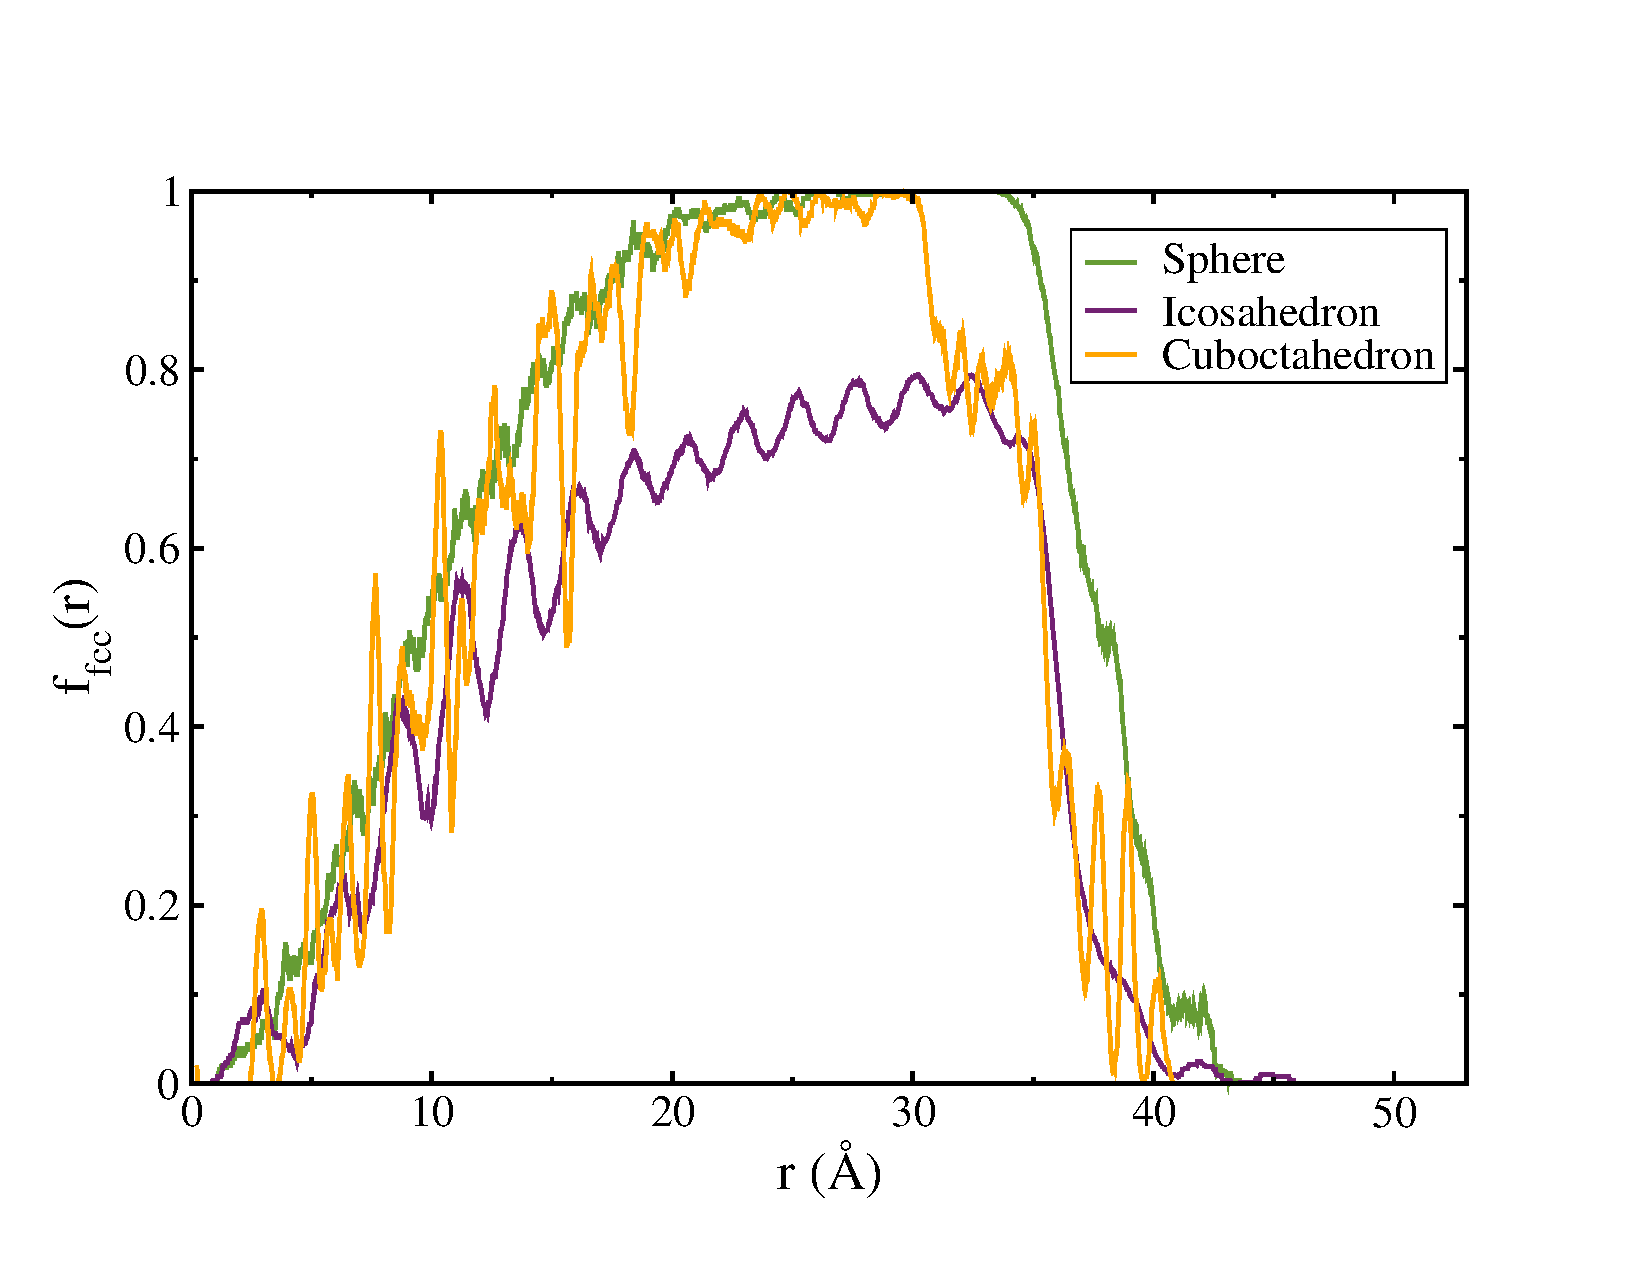
\includegraphics[width=5in]{figures/struct-bowr.pdf}
        \caption{The fraction of FCC-like local environments as a
          function of radius from the center of 40 \AA\ nanoparticles.
          The spheres and cuboctahedra are originally cut from a FCC
          lattice, so the local ordering persists even close to the
          surface.  Icosahedra are constructed as shells surrounding a
          perfectly icosahedral central core of 13 atoms. Non-FCC
          ordering persists throughout these simulations.}
        \label{fig:struct-bowr}
 \end{figure}

%The icosahedra therefore display phonon
%spectra that are enhanced in the higher frequency peaks
%($\sim 130 \text{~cm}^{-1}$) at the expense of the broad
%$\sim 60-80 \text{~cm}^{-1}$ feature.

\begin{figure}
	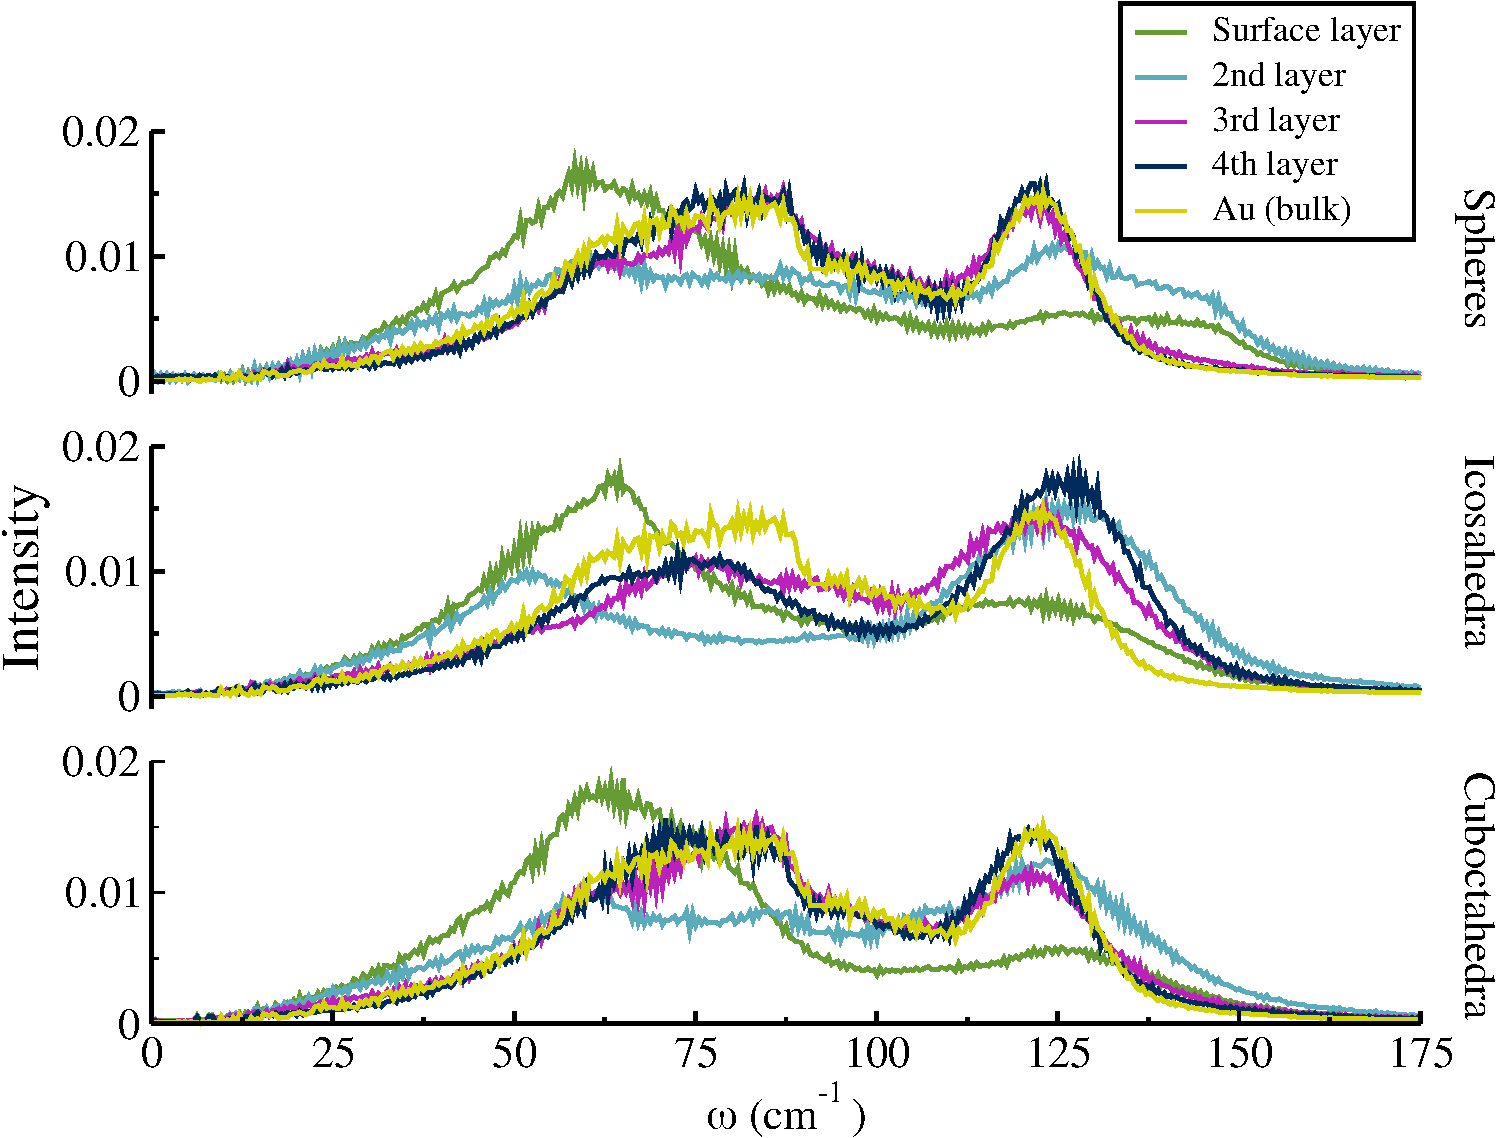
\includegraphics[width=\linewidth]{figures/col-layer40.pdf}
	\caption{The projected vibrational density of states
          (Eq. \ref{eq:DOS}) for individual layers in the largest gold
          nanoparticles (top: spheres, middle: icosahedra, bottom:
          cuboctahedra). In all systems, the surface layer (green) is
          significantly enhanced at low frequencies and is shifted
          down by $\sim~20\text{~cm}^{-1}$. The Au (bulk) curve shown
          for comparison is from a perfect FCC lattice in periodic
          boundary conditions.}
	\label{fig:layer}
\end{figure}

Comparison of the vibrational density of states of all the gold atoms
displays some important differences between the icosahedral structures
and the FCC-based spheres and cuboctahedra
(Fig. \ref{fig:all-v-surf}).  Icosahedral particles have non-FCC
ordering deep into the particle, and this manifests as a shift in
phonon population from the broad low-frequency region to the higher
frequency peak, even for the largest of the particles that were
studied.  For comparison, the largest spheres and icosahedra have only
slight differences in their ``bulk'' phonon density of states.

At the surfaces of the particles, the differences are nearly all in
the higher frequency portion of the spectrum ($>100 \text{cm}^{-1}$),
indicating that the surface undercoordination primarily alters
high-frequency transmission into the solvent.  This suggests roles for
bulk crystalline ordering as well as surface undercoordination in any
model for the interfacial thermal conductance.

\begin{figure}
	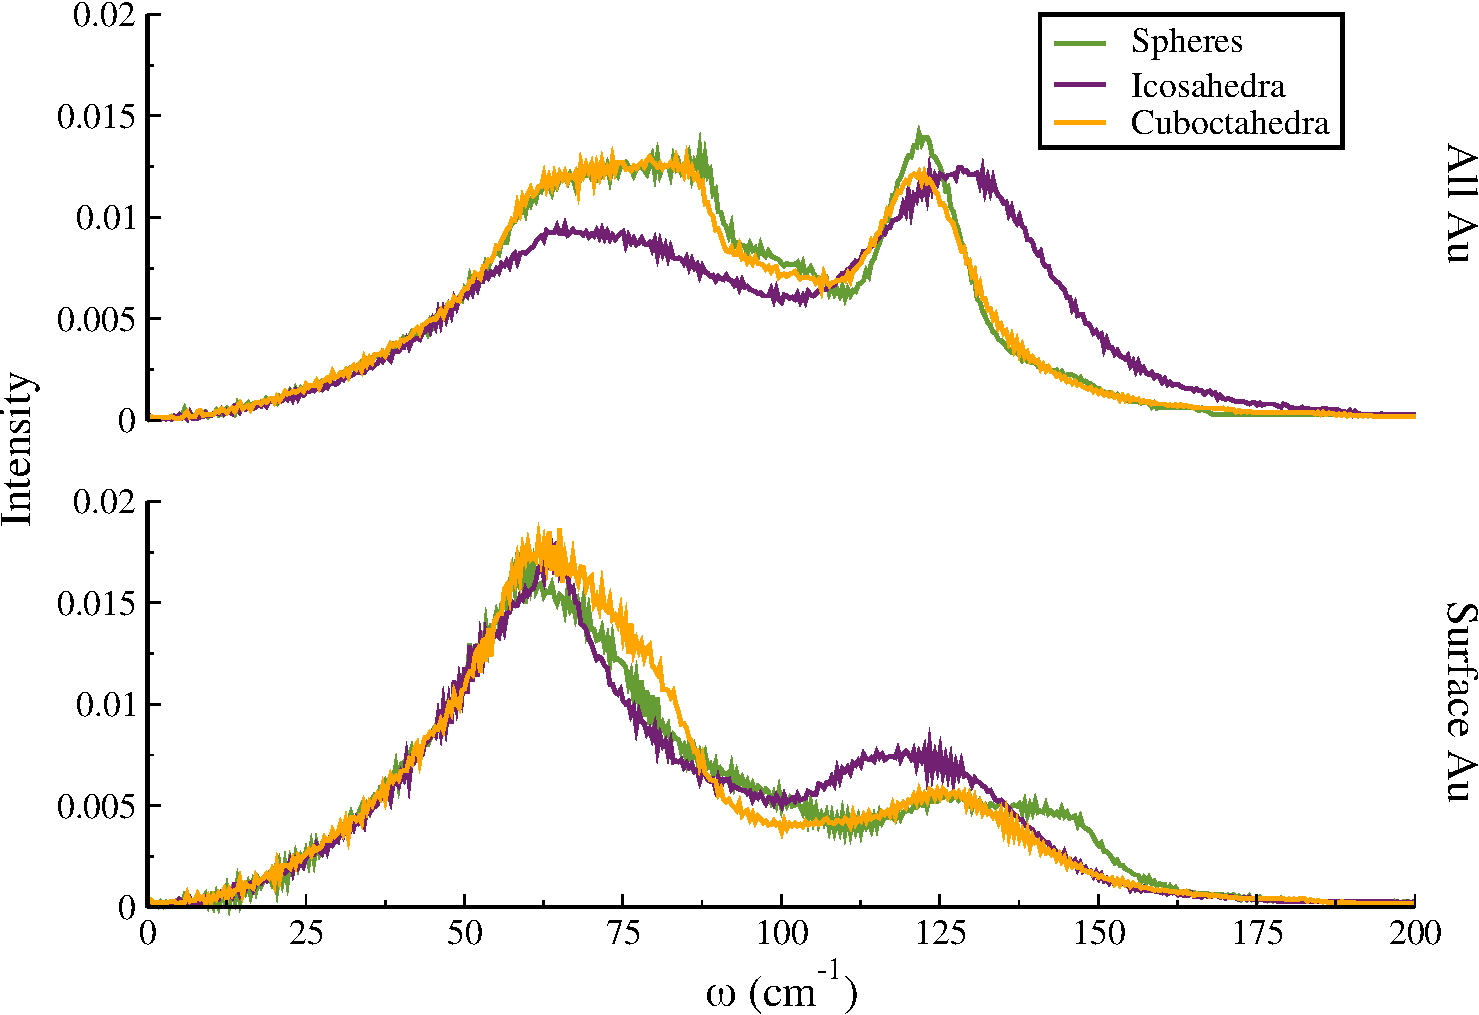
\includegraphics[width=\linewidth]{figures/all-v-surface.pdf}
	\caption{The projected vibrational density of states for all
          gold atoms (top panel) shows that the phonons in FCC-like
          nanoparticles (spheres, cuboctahedra) have similar frequency
          representation, while the non-FCC structures (icosahedra)
          have significantly altered ``bulk'' spectra. For surface
          atoms (bottom panel), the differences in surface
          undercoordination  appear at higher frequencies.  These
          spectra were computed for the largest particles in each of
          the different morphologies.}
	\label{fig:all-v-surf}
\end{figure}

Except in the case of the icosahedra, vibrational power spectra that
include all gold atoms in the nanoparticles do not show significant
dependence on particle radius (see Fig. \ref{fig:all-spect}.  This
suggests that mismatch models (like AMM or DMM) that use only bulk
properties will not be able to capture the surface behavior that is
relevant to heat transfer at the nanoscale.

%Projecting out the phonon contributions that are normal to the interface and assuming that phonon group velocity is always tied to the bulk speed of sound leads us to a relatively simple phonon transmission model,
% \begin{equation}
% \tau_{a \rightarrow b}(\omega) = \frac{v_b \rho^\perp_b(\omega)}{v_a \rho^\perp_a(\omega) + v_b \rho^\perp_b(\omega)}
% \label{eq:transmission}
% \end{equation}
% where $v_a$ and $v_b$ are the speeds of sound in the two materials.  We have used $v_\text{Au} = 3240 \text{~m s}^{-1}$ and $v_\text{hexane} = 1122 \text{~m s}^{-1}$ for hexane at similar conditions.\cite{CRC,Ball2001}  $\rho^\perp(\omega)$ is the projected density of states, and it is proposed that the density of states should include only the atoms at the interface that are in \textit{direct physical contact}, i.e. the surface layer of gold atoms and hexane within 5 \AA\ of the gold particle. 

% The frequency-dependent transmission probabilities computed using these assumptions are shown in Fig. \ref{fig:transmission}. The most important differences appear in the heat-carrying modes below $50 \text{~cm}^{-1}$. For the spherical particles, the transmission probabilities in the low frequency region show the same trend as the thermal conductance ($G$) values.  The low-frequency phonon transmission probabilities increase with particle radius until the particles reach $\sim 20 \text{~\AA}$.  Above this size, transmission in this range has converged to the large particle behavior.  

% The icosahedral particles exhibit much more uniform behavior under this transmission model, with variations only for the smallest particles.  A reasonable explanation for this observation is that the surface layers are dominated by the $\text{CN} = 9$ atoms, which all have similar contributions to the vibrational density of states.

% \begin{figure}
% 	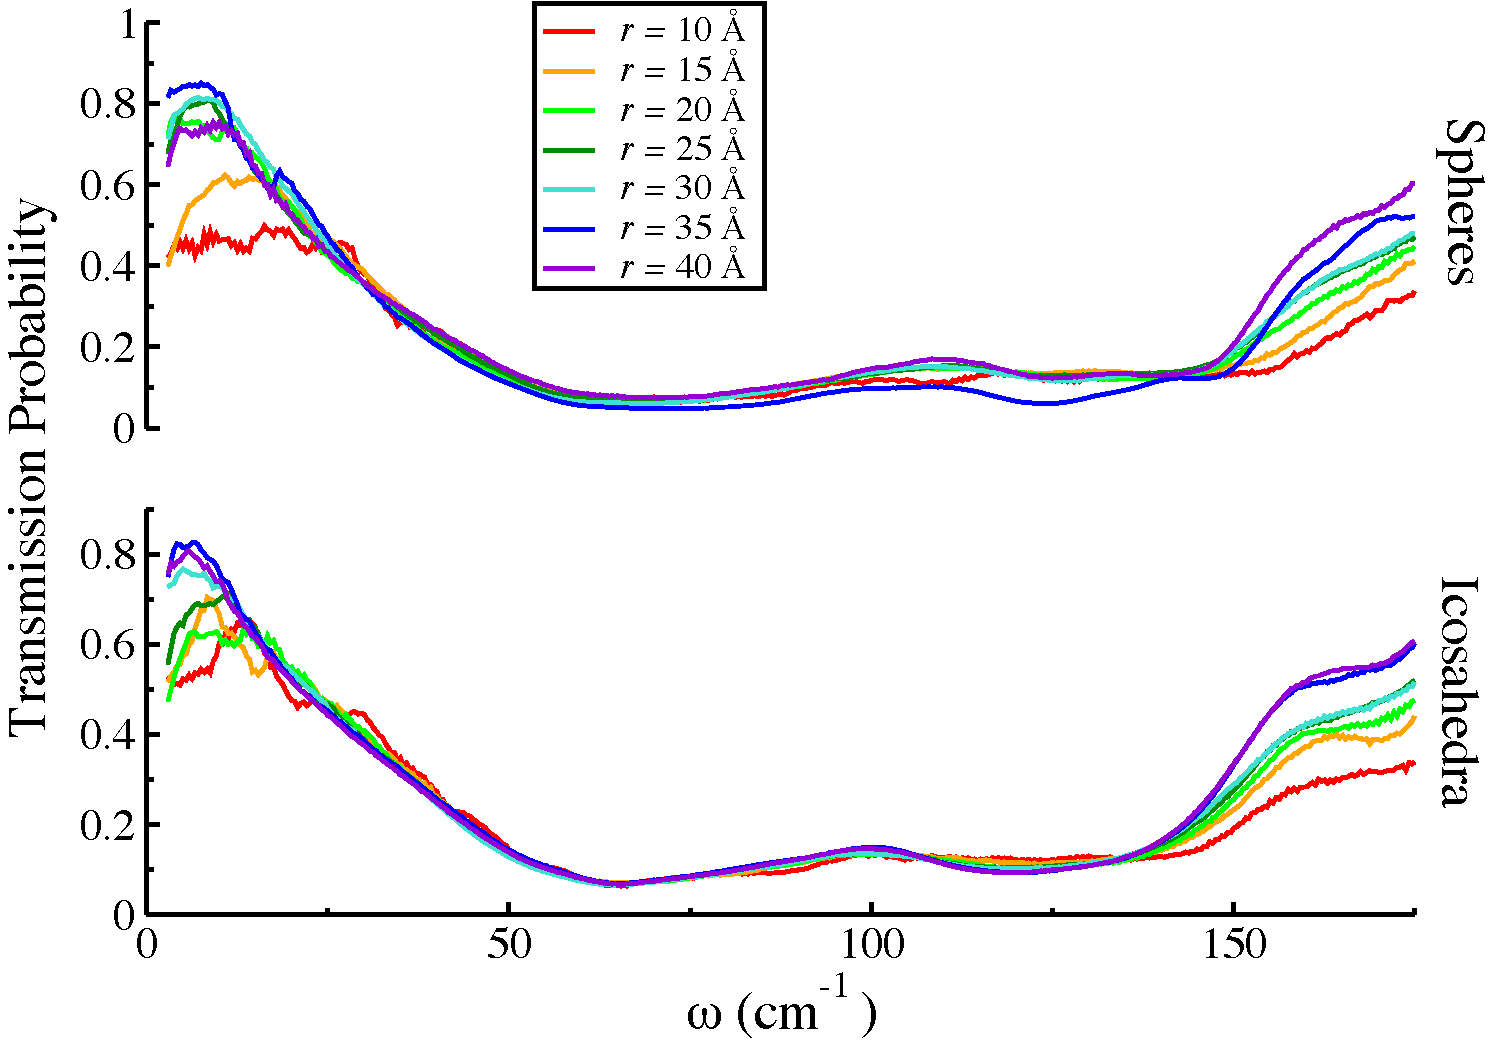
\includegraphics[width=\linewidth]{figures/col-transmission.pdf}
% 	\caption{The frequency-dependent phonon transmission model, Eq. (\ref{eq:transmission}), predicts size-dependent phonon transmission at lower frequencies ($< 50 \mathrm{~cm}^{-1}$), and this effect is particularly pronounced in the spherical nanoparticles.  Icosahedral surfaces are dominated by the $\text{CN} = 9$ atoms, so differences in the low-frequency transmission are diminished.}
% 	\label{fig:transmission}
% \end{figure}

Solvent vibrational densities of states are remarkably similar for the
icosahedral and spherical particles, even for solvent that is within 5
\AA\ of the interface (Fig. \ref{fig:all-spect}). 
While the solvent VDOS in the icosahedral
and spherical systems shows only small changes as a function of
particle size, the solvent in the cuboctahedral systems appears to
shift to lower frequencies with increasing particle radius.  The gold
VDOS in all systems displays a shift from the low frequency peak,
$70 \mathrm{~cm}^{-1}$, to a peak at $125 \mathrm{~cm}^{-1}$ as the
particle radii increases and there is a significant difference between
the two FCC structures and the icosahedra spectra.  The FCC structures
increase in intensity at $125 \mathrm{~cm}^{-1}$ with increasing
particle radius, while the icosahedra VDOS shows a shift in population
from low frequencies to the higher frequency peak.  Note that the gold
shown in Fig. \ref{fig:all-spect} includes all layers of the
particles.

Due to the similarity in solvent VDOS, a model for interfacial 
thermal transport in these
systems would need to include the lattice structure of the particle
and the quantity and solvent accessibility of specific kinds of
undercoordinated metal atoms.

\begin{figure}[!htb]
        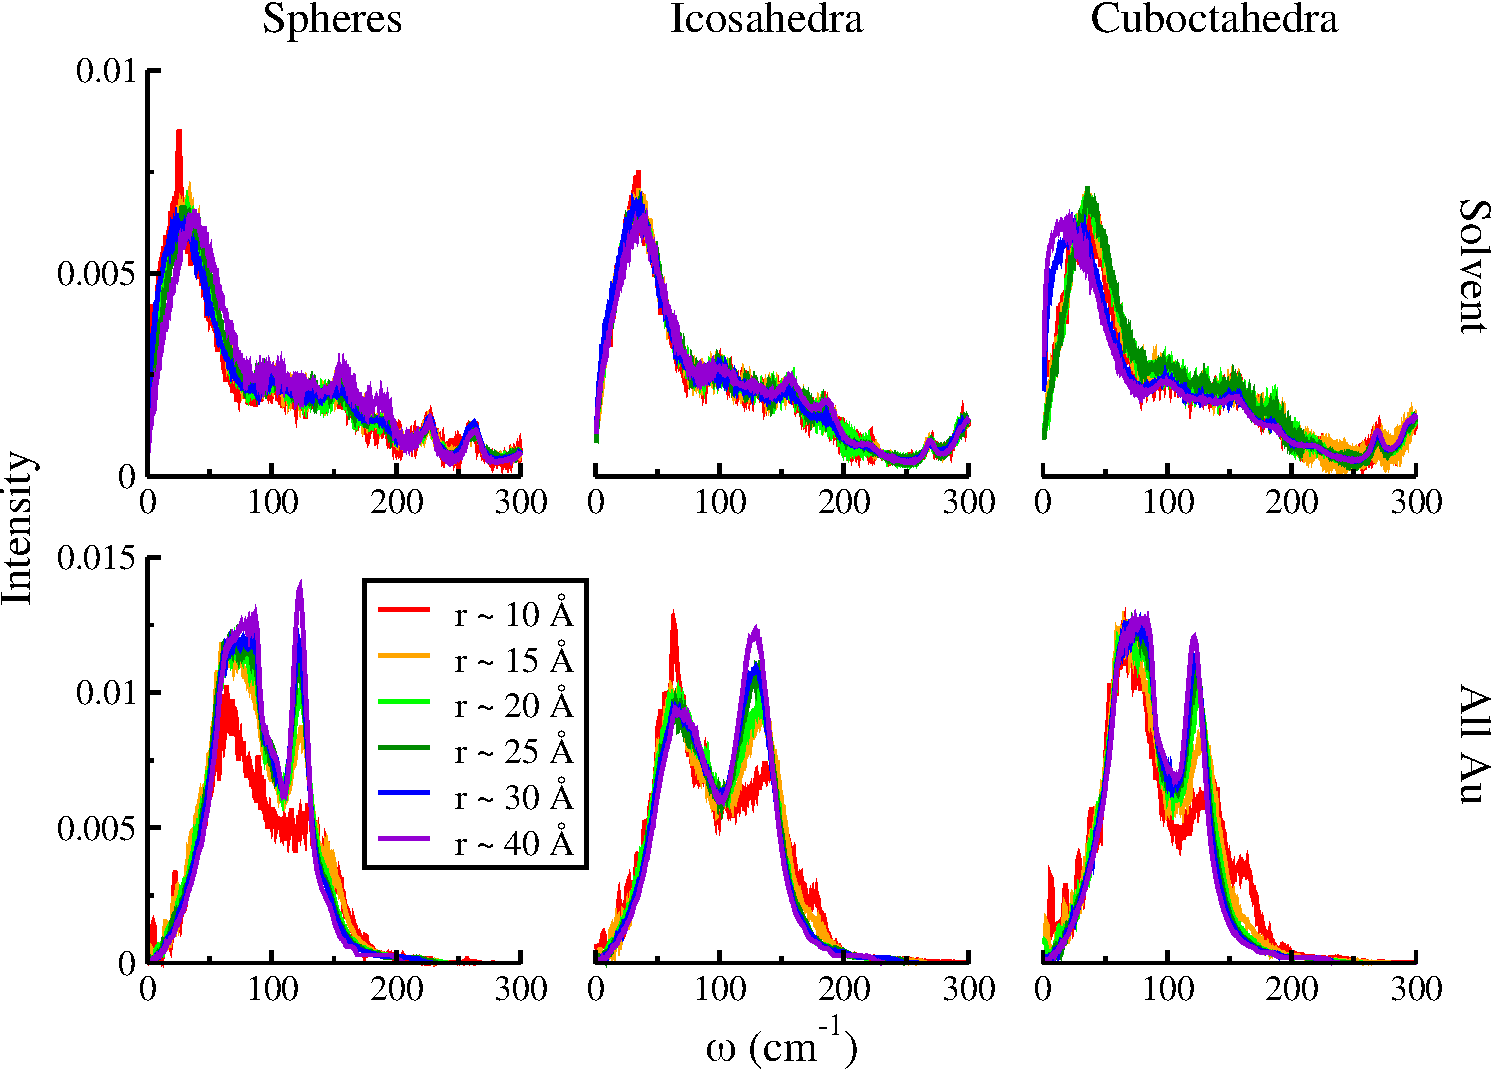
\includegraphics[width=5in]{figures/all-spect.pdf}
        \caption{The normalized low frequency density of states (DOS)
          of the interfacial solvent and the gold particle for the
          icosahedral and spherical systems. }
        \label{fig:all-spect}
\end{figure}

\subsection{A Simple Model for Bare Nanoparticle Conductance}
The vibrational densities of states suggest the bare metallic
nanoparticles exhibit different bulk phonon frequencies that depend on
crystalline packing, and different surface spectra that depend on
surface undercoordination.  Both of the bulk and surface frequencies
can effect thermal transport, so a simple model in terms of a linear 
combination of surface densities of undercoordinated atoms can be explored,
\begin{equation}
G \approx a~\mathrm{CN}_{6} + b~\mathrm{CN}_{7} + c~\left(1+c^{\prime}~\delta_\mathrm{ico}\right)~\mathrm{CN}_{8} + d~\left( 1 + d^{\prime}~\delta_\mathrm{ico} \right)~\mathrm{CN}_{9}
\label{eq:lin-fit}
\end{equation}
where, $a - d$ are coordination transport coefficients with the units
of $10^{-20}$ MW/K and $\mathrm{CN}_{n}$ have surface density units
(1/\AA $^2$) for surface atoms with coordination number $n$.  The
delta function, $\delta_\mathrm{ico}$ is set to unity for icosahedral
structures, and zero for FCC-like nanoparticles.  The coefficients
$c^{\prime}$ and $d^{\prime}$ are weighting factors that recognize the
differences in the bulk density of states in the icosahedral
particles.  Fitting the six parameters was done using a simple
ordinary least squares model with data from all simulated particles.

\begin{table}
\centering
\caption{Parameters of the Model in Eq. (\ref{eq:lin-fit}).
  \label{tab:coeff to fit}}
\begin{tabular}{ cccccc }
\toprule
 $a$ & $b$ & $c$ & $c^{\prime}$ & $d$ & $d^{\prime}$ \\
\midrule
 858.9405 & 183.9062 & 291.7960 & -0.5943 & 369.6250 & -0.2498 \\
\bottomrule
\end{tabular}
\end{table}

With Eq. \eqref{eq:lin-fit} it should be possible to predict the
interfacial thermal conductance for bare gold nanoparticles in hexane
based only on a structural analysis of the surface for coordination
densities and the interior of the particle for crystalline structure.
The predicted (and simulated) values of the thermal conductance are
given in Fig. \ref{fig:models}.  With a coefficient of determination
($R^2$) value of 0.656, this fit does not predict $G$ with a high
degree of certainty, but it does suggest the large role that
undercoordinated surface atoms play in conductance. Coefficients used
in Eq. \eqref{eq:lin-fit} are given in Table \ref{tab:coeff to fit}.

The coefficients provide some information about the thermal transport
capabilities of each type of undercoordinated surface atom. These fits
suggest that severely undercoordinated atoms (CN=6) transfer the
largest amount of heat per atom, although their population in all
systems is low.

It is also important to note that this fit considers the two different
types of particles when finding the best fits for the most populous
surface atoms (CN=8, CN=9).  If the system is FCC-like the weight of
the CN = 8 and CN = 9 are 2.464 and 1.333 times larger than their
contributions from icosahedral cores.

Since the coefficients are related to the amount of energy transfered
per atom type, these atoms on the FCC-like structures transfer a
larger amount than in the icosahedral structure.  This is likely due
to differences in the underlying ``bulk'' densities of states.

\begin{figure}
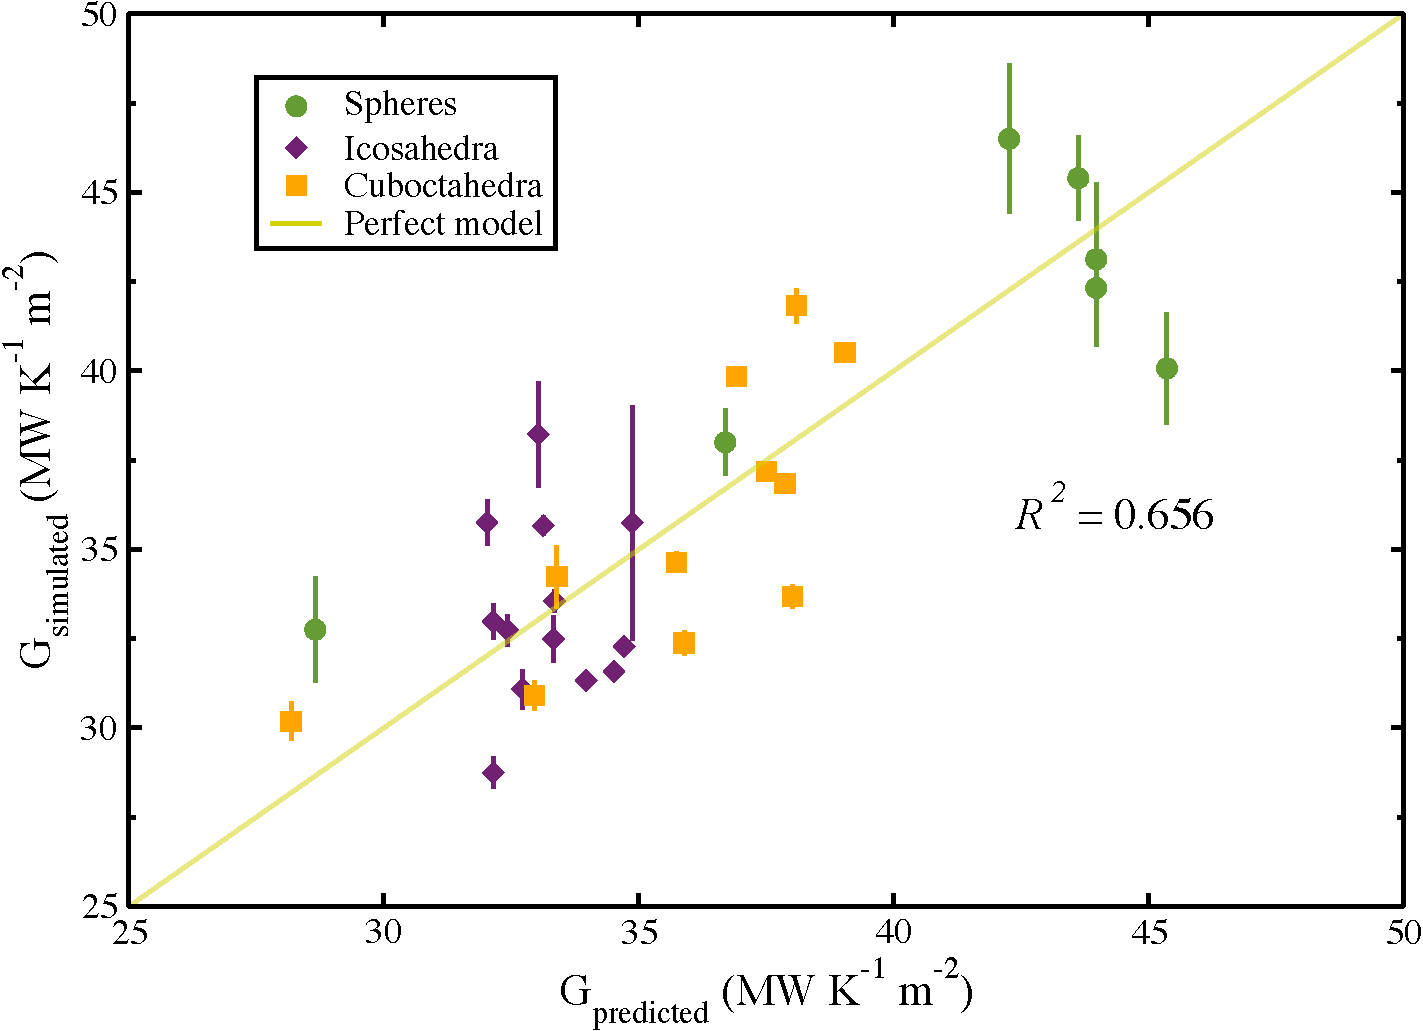
\includegraphics[width=\linewidth]{figures/models.pdf}
 	\caption{Structurally-predicted thermal conductance values from Eq. \eqref{eq:lin-fit} compared with the simulated thermal conductance values. Error bars indicate the standard error computed using five replica simulations. }
    \label{fig:models}
\end{figure}

% The vibrational density of states (VDOS) of the materials at the interface calculates the occupied low frequency phonon modes of the materials.
% As the radii of the particles increases, the VDOS of all gold atoms does not see a significant change below $100$ $cm^{-1}$ in either of the spherical systems, as seen in Supporting Information. 




\section{Conclusions}
The primary observation of this work is that particle morphology has a
significant effect on interfacial thermal conductance from bare
particles to the surrounding solvent.  In particular, spherical and
cuboctahedra particles have a size-dependent interfacial thermal
conductance, while icosahedral particles conduct heat to the
surrounding solvent only slightly better than the flat (111) facets.

This work explored one explanation for this difference in terms of the
density of undercoordinated sites on the surfaces of these three
particle morphologies. Nanospheres, because they are carved out of an
underlying FCC lattice, expose significantly undercoordinated atoms
($\text{CN} = 6-8$) to the solvent. For very small spheres,
microfacets of (111), (100), and (110) dominate the surface, but for
larger particles, the density of undercoordinated atoms becomes a
significant fraction of the exposed atoms.  In large icosahedral
particles, the particles are dominated by (111) faces, and the
$\text{CN} = 9$ atoms dominate the surface.  Similarly, in large
cuboctahedral particles, the (111) and (100) facets are both present,
and the $\text{CN} = 9$ and $\text{CN} = 8$ atoms share the particle
surface in a 2:3 ratio. Surface atom undercoordination leads directly
to changes in the surface vibrational density of states, particularly
at frequencies around $\sim 150 \text{~cm}^{-1}$.  The linear model
suggests that differences in surface atom undercoordination
(particularly for atoms that are undercoordinated relative to a flat
facet) may be largely responsible for thermal conductivity trends in this work.

This is not a complete explanation for the conductance values,
however, as the large icosahedral particles exhibit $G$ values above
the planar (111) facet, and large cuboctahedra have $G$ values above
\textit{both} the (111) and (100) facets.  Edge and vertex atoms in
these clusters may play an outsized role, and collective low-frequency
modes of the particles may also be important, as the underlying
``bulk'' density of states also depends on particle morphology.

%Transmission models should therefore take both surface coordination and surface proximity into account when estimating energy transfer between materials.
%%%%%%%%%%%%%%%%%%%%%%%%%%%%%%%%%%%%%%%%%%%%%%%%%%%%%%%%%%%%%%%%%%%%%%%%%%%%%%%%%%%
%		COMPUTATIONAL DETAILS
%%%%%%%%%%%%%%%%%%%%%%%%%%%%%%%%%%%%%%%%%%%%%%%%%%%%%%%%%%%%%%%%%%%%%%%%%%%%%%%%%%%


%\begin{acknowledgement}
%  Support for this project was provided by the National Science
%  Foundation under grant CHE-1362211 and CHE-1663773. Computational
%  time was provided by the Center for Research Computing (CRC) at the
%  University of Notre Dame.
%\end{acknowledgement}
%
%\begin{suppinfo}
  %Details of system composition, surface densities of undercoordinated
  %atoms for ideal particle geometries, vibrational densities of states
  %for undercoordinated sites, fractional FCC ordering for particles,
 % and information on the linear model for thermal conductance.
%\end{suppinfo}

%\newpage

%\bibliography{Morph}

%\end{document}


%%%%%%%%%%%%%%%%%%%%%%%%%%%%%%%%%%%%%%%%%%%%%%%%%%%%%%%%%%%%%%%%%%%%%%%%%%%%%%%%%%%
%		CHAPTER 4 -- Staple Motifs
%%%%%%%%%%%%%%%%%%%%%%%%%%%%%%%%%%%%%%%%%%%%%%%%%%%%%%%%%%%%%%%%%%%%%%%%%%%%%%%%%%%
\chapter{A PREDICTION OF THE THERMAL CONDUCTIVITY OF \ce{Au144PET60} NANOARRAYS}\label{chap:arrays}
\section{Introduction}
Thiolated gold nanocluster have been studied in great detail both experimentally and theoretically.\cite{Hakkinen2012, Sardar2009, Jin2010, Tsukuda2012}
The electronic,\cite{Lopez-Acevedo2011,Walter2008} optical,\cite{Cui2014} and catalytic properties;\cite{Chen2013, Lopez-Acevedo2010} promising to make them building blocks for nanotechnology applications.\cite{Dong2011,Podsiadlo2010,Shevchenko2006,Talapin2010}
These properties depend on sites of the particles, as well as the ligand identities.
Nanocrystal arrays, which are close-packed structures of nanoparticles in a colloidal solution, have been proposed as alternatives for more expensive single-cystal semiconductor materials in transistors,\cite{Talapin2005} memory devices,\cite{Sun1999} solar cells,\cite{Tang2011,Gur2005,Ehrler2012} and thermoelectrics.\cite{Ong:2013rt,Kovalenko2010,Wang2008,Ko2011} 

One of the first theoretical studies of nanocrystal arrays was performed by Luedtke and Landman.\cite{Luedtke1996}
They examined small clusters with alkanethiol ligands on a graphite surface and in superlattices. 
A more recent experimental study by Liu \textit{et al.} explored the effect of surface chemistry on the thermal conductivity of a nanocrystal array.\cite{Liu2015}
The study by Liu \textit{et al.} varied nanocrystal core size, the binding group of the ligand, and the ligand length. The primary finding was that with a decrease in ligand length or an increase in the core size, the thermal conductivity of the array increased.
The volume fraction of the insulating material (the ligand) is reduced in both of those cases.

Similar results with respect to the core diameter have been seen in theoretical studies of nanocrystal arrays by Ong \textit{et al.}\cite{Ong:2014yq} and Zanjani \textit{et al.}\cite{Zanjani2014} 
In particular Ong \textit{et al.} found that in nanocrystal arrays, vibrational states are able to elastically couple across the interfaces, yielding a thermal conductivity that is dependent on the density of the ligand layer.\cite{Ong:2014yq} The coupling was further studied by varying the core atomic mass and finding the relationship between core vibrational states and the interfacial thermal conductivity.

The study by Zanjani \textit{et al.} on gold nanocrystals with hexylthiol capping ligands varied both core size and ligand density.\cite{Zanjani2014}
The phonon dispersion of the superlattice structures was obtained and the thermal conductivity of the nanocrystal arrays displayed the same trends oberved by Liu \textit{et al.} that is, an increase in thermal conductivity of the array with decreased volume percentage of the ligand layer.\cite{Liu2015} 

All the nanoparticles previously studied contain less than 500 atoms. Recent work by Pohjolainen \textit{et al.} provides structures and force field parameters based upon crystal structures for thiolated gold nanoclusters found in a matching crystalography study of the clusters in arrays.\cite{Pohjolainen2016} 
These structures contain individual particles as well as nanoarrays, with the largest of the structures containing 144 \ce{Au} atoms. All of the characterized nanoclusters have a ``staple''-motif ligand that was shown to be thermally stable in this model. Many of the parameters were taken from work from Banerjee \textit{et al.} that explored \ce{Au25} and \ce{Au38} nanoclusters.

The staple motif in these nanoclusters presents an interesting test for theories of thermal transport. 
The staple motif has three gold atoms (for the largest particle), two of the gold atoms in the staple are in direct contact with the core of the particle, while the remaining atom resides in the ligand layer, but is bonded to sulfur atoms. In our previous work on the effect on thermal properties due to under-coordination of gold atoms the surface,\cite{Neidhart2017} the gold atoms within the staple motif may present interesting challenges. 
For this reason, we have looked at single particles and arrays of \ce{Au144PET60} clusters in two solvents, and look for agreement with the Hasselman and Johnson equation for thermal conductivity in composite materials.\cite{Hasselman}
\subsection{Theory}
Hasselman and Johnson first proposed a predictive formula for the effective thermal conductivity of a composite material using known bulk properties of the two complinents separately.\cite{Hasselman}
The original formulation of the Hasselman and Johnson equation for the effective thermal conductivity of the composite,
\begin{equation}
\label{eq:composite}
    \lambda_e = \lambda_s \bigg( \frac{\lambda_p (1+2\alpha)+2\lambda_s +2v_p[\lambda_p(1-\alpha)-\lambda_s]}{\lambda_p (1+2\alpha)+2\lambda_s -v_p[\lambda_p(1-\alpha)-\lambda_s]} \bigg)
\end{equation}
uses $\lambda_p$ and $\lambda_s$, the particle and solvent thermal conductivities, and $v_p$, the volume fraction of the nanoparticles. $\alpha$ is the interfacial term, which
is a dimensionless factor that relates the thermal boundary resistance to the radius of the particles.
The thermal boundary resistance in this work is
\begin{equation}
    \alpha = \frac{R_{TBR}}{r_p} = \frac{\lambda_s}{Gr_p}
\end{equation}
where $G$ is the interfacial thermal conductivity from the particle to the solvent, and $r_p$ is the radius of the particle.
Modifications to the Hasselman and Johnson equation have been made by Minnich \textit{et al.} to include an interface density for the spherical particles and a more formal volume fraction of the nanoparticles.\cite{Minnich2007}

Each portion of Eq. \ref{eq:composite} can be calculated separately in order to predict a composite material thermal conductivity. 
The volume fraction of the particles can be found through geometric means using the information about the particles in the array.
The thermal conductivity of the solvent, $\lambda_s$ , can be found through simulations of bulk solvent. 
Similarly, $\lambda_p$ can be calculated from bulk simulations of the core material of the particle. 
The most difficult piece to obtain is the $\alpha$ term, where the interfacial thermal conductance of the particles is the primary quantity of interest.
The interfacial thermal conductance of the nanoclusters investigated in this work were found using the same method as Stocker \textit{et al.} for nanospheres.\cite{Stocker2016}

Molecular modelling of heat conduction in nanoarrays considers only one method for thermal transport: conduction.
This work is a purely classical approximation of nanoarrays and does not consider electronic effects (such as polarization of the gold surface) or radiative transfer. 
While convection may be seen through classical simulations, it is not likely to be a large contribution to thermal transport in a densely-packed array. 
%Additionally, the solvent between the particles in the arrays could display altered diffusion coefficients due to confinement and change in temperature.
%Any coupling in these systems between the gold particles could only be seen through a classical means and the electronic contributions are not considered.
\section{Computational Details}
Nanoarrays of \ce{Au_144PET_60} solvated with either toluene or dichloromethane were simulated using reverse nonequilibrium molecular dynamics (RNEMD).
Individual components of these systems: e.g. single particles in each solvent, pure solvent, and liquid gold were also prepared and simulated using RNEMD.
The following sections describe the potentials used for the interactions in the system as well as how the systems were prepared.

\begin{figure}
    \centering
    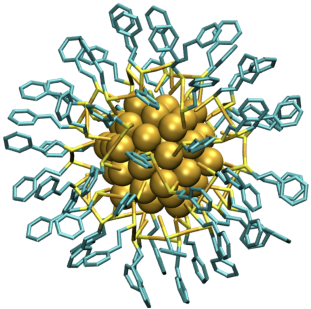
\includegraphics[scale=3]{figures/Au144-part.pdf}
    \caption{A single \ce{Au144PET60} cluster with the icosahedral core atoms rendered as spheres. All atoms in the ligand staple motof are displayed as stick like structures for clarity of the particle structure.}
    \label{fig:single-part}
\end{figure}

\subsection{Force Fields}
In the single particle systems and the liquid gold simulations, the gold--gold interactions are modeled using the quantum Sutton-Chen (QSC) potnetial.\cite{Qi:1999ph}
In the \ce{Au_144PET_60} particle, there are three distinct gold atom types: \ce{Au_{body}}, \ce{Au_{surface}}, and \ce{Au_{ligand}}. 
The gold interior to the particle, the icosahedral core, is defined as an \ce{Au_{body}} atom.
The other two gold atom types are part of the ligand staple motif and are directly bonded to sulfur atoms.
\ce{Au_{surface}} is the gold in the staple motif that is in direct contact with the surface of the particle. 
\ce{Au_{surface}} is treated with QSC for the interactions with \ce{Au_{body}} but with a Lennard-Jones potential for interactions with \ce{Au_{ligand}}, which is further from the surface of the particle and bonded between two sulfur atoms.
\ce{Au_{ligand}} is treated as a purely Lennard-Jones atom with parameters from Pohjolainen \textit{et. al.}.\cite{Pohjolainen2016}
All parameters for the staple motif use parameters from Pohjolainen \textit{et. al.}\cite{Pohjolainen2016} and Banerjee \textit{et al.}\cite{Banerjee2012} in addition to parameters from TraPPE-UA\cite{TraPPE-UA.alkanes,TraPPE-UA.alkylbenzenes} which can be found in Table \ref{tab:staple-parameters}.

\begin{figure}
    \centering
    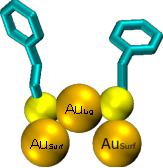
\includegraphics[scale=2]{figures/single.pdf}
    \caption{The \ce{Au} and \ce{S} atoms in the staple motif are depicted with spheres, while the \ce{PET} R groups are shown as stick like structures for clarity of the staple structure. The \ce{Au_{surf}} atoms sit directly on the icosahedral core of the nanocluster, while the \ce{Au_{lig}} atom is slightly out from the gold surface and are bonded to the sulfur atoms in two \ce{PET} ligands.}
    \label{fig:staple}
\end{figure}
\begin{landscape}
\begin{table}[]
\centering
\caption{Composition of a single nanoparticle and non-bonded interactions parameters for the interaction with gold. \label{tab:staple-parameters}}
\begin{tabular}{ c|ccccccl }
 \toprule
Sites & atoms & mass & $\sigma_{ii}$ & $\epsilon_{ii}$ & $\sigma_{\ce{Au}-i}$ & $\epsilon_{\ce{Au}-i}$  & source \\
     && (amu)& (\AA)        & (kcal/mol)     & (\AA)             &  (kcal/mol)          &  \\
\hline
 \ce{Au_{body}} &54&196.97&&\multicolumn{2}{c}{parameters from QSC}&\\
 \ce{Au_{surface}} &60&196.97&&\multicolumn{2}{c}{parameters from QSC}&\\
 \ce{Au_{ligand}} &30&196.97&2.629&5.2899&2.629&5.2899&Refs. \protect\cite{Pohjolainen2016} and \protect\cite{Banerjee2012}\\
 S           &60& 32.0655  & 4.45  & 0.2504 & 2.40   & 8.465  & Refs. \protect\cite{landman:1998} ($\sigma$) and \protect\cite{vlugt:cpc2007154} ($\epsilon$) \\
 \ce{CH2}    &120& 14.03    & 3.95  & 0.09141& 3.54   & 0.1749 & Refs. \protect\cite{TraPPE-UA.alkanes}, \protect\cite{vlugt:cpc2007154} and \protect\cite{landman:1998}\\
 CHar        &360& 13.02    & 3.695 & 0.1004 & 3.4625 & 0.1680 & Refs. \protect\cite{TraPPE-UA.alkylbenzenes} and \protect\cite{vlugt:cpc2007154}\\
 \bottomrule
\end{tabular}
\end{table}
\end{landscape}

To model solvents, dichloromethane and toluene, and the organic ligands, we use parameters from united atom models.
Dichloromethane is modeled with united atom Lennard-Jones atoms and charges taken from Meyer \textit{et. al.}\cite{Meyer1978} while the intramolecular parameters use harmonic force constants are adopted from OPLS-AA.\cite{Jorgensen98a}
Toluene is modeled as a rigid body using parameters from TraPPE-UA.\cite{TraPPE-UA.alkylbenzenes} %(From TraPPE-UA JPCB 104, 8008)
In the ligand staple motif, the carbon atoms were treated with TraPPE-UA,\cite{TraPPE-UA.alkanes,TraPPE-UA.alkylbenzenes,TraPPE-UA.thiols} while the sulfur parameters we adopted from TraPPE-UA\cite{TraPPE-UA.thiols} while bonds, bends, and torsions for the staple are adopted from Pohjolainen \textit{et al}.\cite{Pohjolainen2016}

Non-bonded interactions between the staple motif and icosahedral core of the particles are modeled using parameters derived from adsorption studies of thiolates on Au surfaces.
The S—-Au non-bonded parameters are adopted from work from Luedtke and Landman.\cite{landman:1998}

Other interactions between Au and non-metal atoms in the staple ligand are adapted from an adsorption study by Vlugt \textit{et. al.},\cite{vlugt:cpc2007154} of alkyl thiols on gold surfaces. The parameters are from a pair-wise Lennard-Jones potential for the interaction between Au and $\mathrm{CH}_x$ and S based upon the Hautman and Klein potential for Au(111) surfaces.\cite{hautman:4994}
The non-bonded interactions between gold atoms and toluene solvent use parameters from the same work.
Au and dichloromethane interactions use the aforemented work from Vlugt for the central carbon and the Au-Cl interactions through Johnson or Lorentz-Berthelot mixing rules.\cite{Johnson89}

\begin{table}
%\bibpunct{}{}{,}{n}{}{,}
\centering
\caption{Harmonic bond parameters for different components in the simulated systems. %The first part of the table are the atoms in the staple motif within the nanoparticle. The latter sections are the solvents: toluene and dichloromethane, respectively.
 \label{tab:abond}}
\begin{tabular}{ cc|ccl }
 \toprule
 $i$&$j$ & $r_0$ & $k_\mathrm{bond}$ & source \\
    &    & (\AA) & $(\mathrm{~kcal/mole/\AA}^2)$ & \\
\hline
\ce{Au$_{surf}$}   & \ce{S} &  2.41  &  150 & Ref. \protect\cite{Pohjolainen2016}\\
\ce{Au$_{lig}$}   & \ce{S} &  2.33  &  150 & Ref. \protect\cite{Pohjolainen2016}\\
S          & \ce{CH2} & 1.820   & 444  & Refs. \protect\cite{TraPPE-UA.thiols} and \protect\cite{Jorgensen:1996sf} \\
%\ce{CH3}   & \ce{CH2} & 1.540   & 536  & Refs. \protect\cite{TraPPE-UA.alkanes} and \protect\cite{Jorgensen:1996sf} \\
\ce{CH2}   & \ce{CH2} & 1.540   & 536  & Refs. \protect\cite{TraPPE-UA.alkanes} and \protect\cite{Jorgensen:1996sf} \\
CHar & \ce{CH2} & 1.540   & 536  & Refs. \protect\cite{TraPPE-UA.alkylbenzenes} and \protect\cite{Jorgensen:1996sf}\\
CHar       & CHar     & 1.40    & 938  & Refs. \protect\cite{TraPPE-UA.alkylbenzenes} and \protect\cite{Jorgensen:1996sf} \\
%\hline\hline
CHar       & CHar     & 1.40    & 938  & Refs. \protect\cite{TraPPE-UA.alkylbenzenes} and \protect\cite{Jorgensen:1996sf} \\
CHar       & \ce{CH3} & 1.540   & 536  & Refs. \protect\cite{TraPPE-UA.alkylbenzenes} and \protect\cite{Jorgensen:1996sf}\\
%\hline\hline
Cl      & \ce{CH2}   & 1.40    & 938  & Ref. \protect\cite{Meyer1978}\\
 \bottomrule
\end{tabular}
%\bibpunct{[}{]}{,}{n}{,}{,}
\end{table}

\begin{table}
%\bibpunct{}{}{,}{n}{,}{,}
\centering
\caption{Bend angle parameters for a harmonic potential. The central atom in the bend is atom $j$. 
%The table is structured with the particle staple motif in the first section, followed by the solvents: toluene and dichloromethane.
\label{tab:abend}}
\begin{tabular}{ ccc|ccl }
\toprule
 $i$&$j$&$k$ & $\theta_0$ & $k_\mathrm{bend}$ & source\\
    &   &    & ($\degree$) & (kcal/mol/rad\textsuperscript{2}) & \\
\hline
Au$_{surf}$ & S & Au$_{lig}$  & 91.3 & 460.24 & Ref. \protect\cite{Banerjee2012}\\
S& Au$_{lig}$ & S  & 172.24 & 240.24 & Ref. \protect\cite{Banerjee2012}\\
Au$_{surf}$ & S & \ce{CH2} & 111.6 & 146.37 & Ref. \protect\cite{Banerjee2012}\\
Au$_{lig}$ & S & \ce{CH2} & 106.8  & 146.37 & Ref. \protect\cite{Banerjee2012}\\
S & \ce{CH2} & \ce{CH2}& 114.0   &   124.20& Ref. \protect\cite{TraPPE-UA.thiols}\\
\ce{CH2} & \ce{CH2}  & CHar& 114.0   &   124.20& Ref. \protect\cite{TraPPE-UA.thiols}\\
\ce{CH2} & CHar     & CHar  & 120.0   &   140.0 & Refs. \protect\cite{TraPPE-UA.alkylbenzenes} and \protect\cite{Jorgensen:1996sf}\\
CHar     & CHar     & CHar      & 120.0   &   126.0 & Refs. \protect\cite{TraPPE-UA.alkylbenzenes} and \protect\cite{Jorgensen:1996sf}\\
%\hline \hline
\ce{CH3}     & CHar     & CHar  & 120.0   &   140.0 & Refs. \protect\cite{TraPPE-UA.alkylbenzenes} and \protect\cite{Jorgensen:1996sf}\\
%CHar     & CHar     & CHar      & 120.0   &   126.0 & Refs. \protect\cite{TraPPE-UA.alkylbenzenes} and \protect\cite{Jorgensen:1996sf}\\
%\hline\hline
Cl & \ce{CH2} & Cl & 111.8 & 155.39 &Ref. \protect\cite{Meyer96}\\
 \bottomrule
\end{tabular}
%\bibpunct{[}{]}{,}{n}{,}{,}
\end{table}

\subsection{Simulation Protocol}
The gold particle simulations are started from crystal structures provided in work from Pohjolainen \textit{et. al}.\cite{Pohjolainen2016}
The crystal structures were thermalized to 250K then solvated using Packmol\cite{packmol} with either dichloromethane or toluene molecules that were also equilibrated to 250K.
The solvent sphere was created to be at least 3x the radius of the particle with the solvent maintaining bulk density near the interface (see Table \ref{tab:solvated-part-comp} for exact packing).
At least 7 separate statistically independent configurations of the nanoparticles were created.

Solvated particles were then brought to 250K using the Langevin Hull ensemble.\cite{Vardeman2011} 
Once equilibrated with thermal coupling to the bath for at least 1 ns, the system was simulated without coupling to the bath for 1 ns. 
The particles were then simulated using RNEMD for 1 ns where a thermal flux was applied to create a radially-decaying temperature gradient. 
\begin{figure}
    \centering
    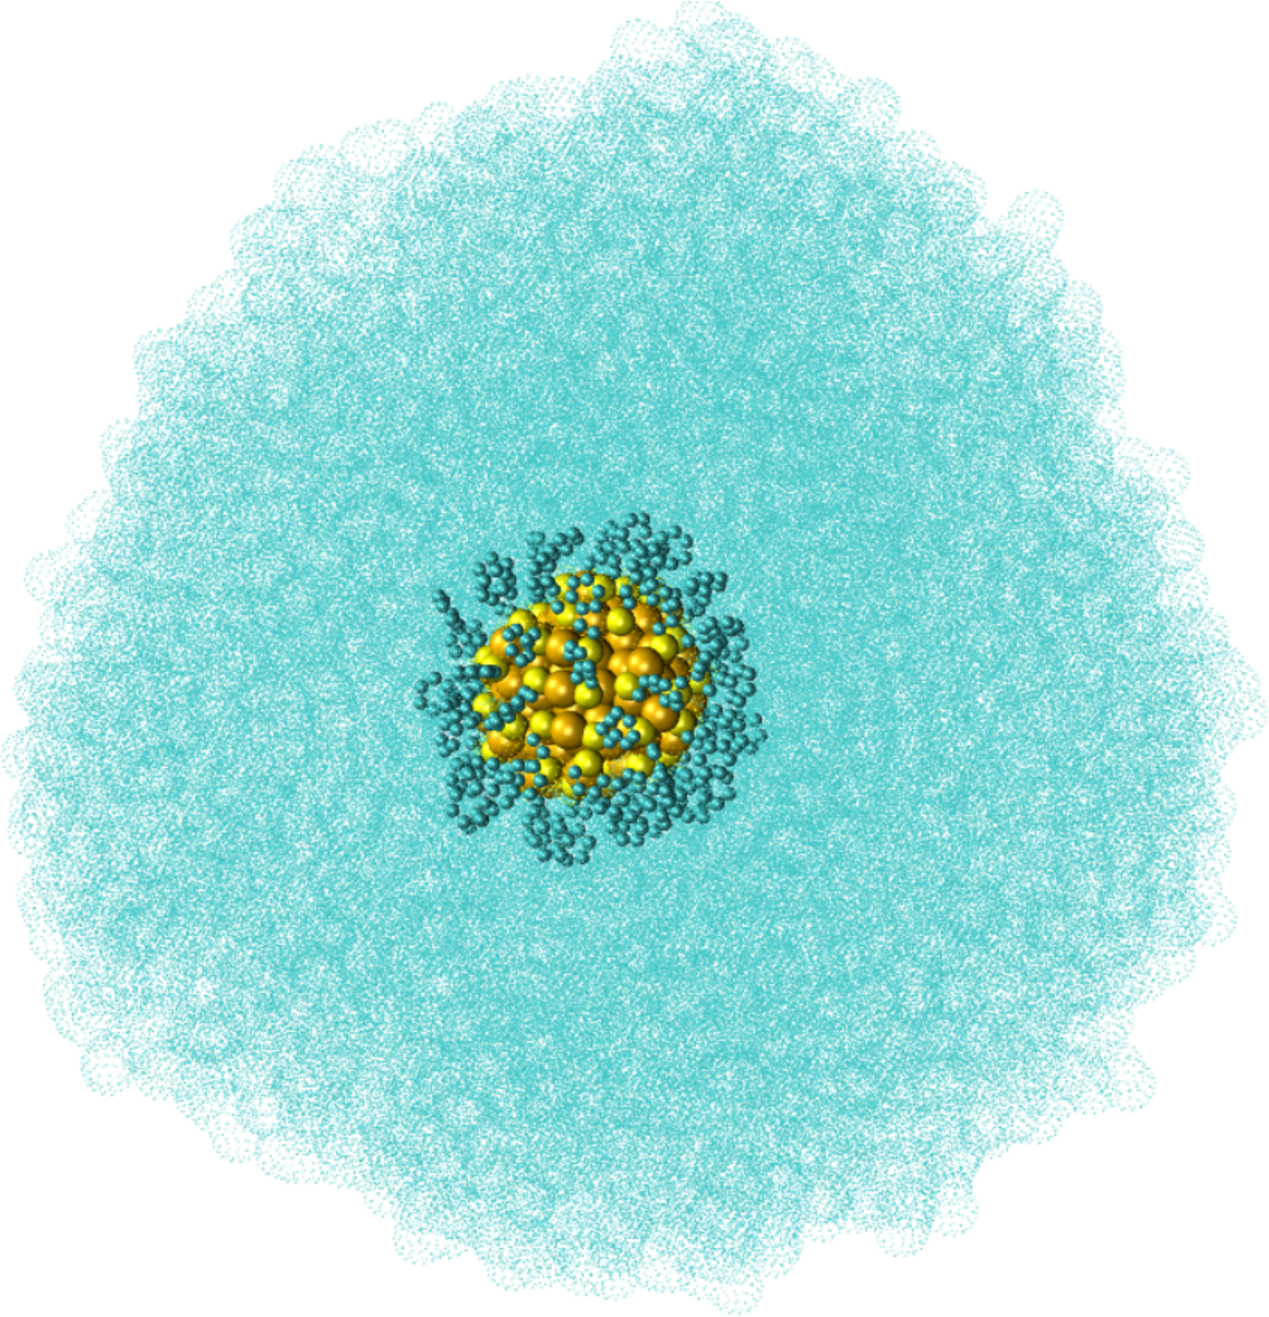
\includegraphics[scale=0.4]{figures/dcm-part.pdf}
    \caption{ A single \ce{Au144PET60} cluster in a solvent cloud of dichloromethane.}
    \label{fig:lambda-bulk}
\end{figure}

Pure solvent simulations were prepared using the bulk solvent density. 
Five statistically independent simulations for each of the three different simulation box lengths.
These simulations were equilibrated to 250K using the canonical (NVT) ensemble for at least 1 ns followed by further relaxation in the (NPT) ensemble for 1 ns.
Finally, the pure solvent systems were equilibrated for at least 1 ns in the microcanonical (NVE) ensemble before undergoing a 10 ns RNEMD simulation.

The pure gold systems followed the same protocol as the dichloromethane and toluene systems, except the temperature for the pure gold system is 1500K, above the melting point of bulk gold.
After equilibration, the relevant thermal flux was applied for 3 ns.
To achieve a similar temperature gradient across the three box sizes (for all bulk simulations), the applied thermal flux was adjusted, see Table \ref{tab:bulk-comp}.
Depending on the size of the simulation box, longer times are needed to allow a steady state temperature gradient to develop, so all systems were run for the duration needed to achieve this steady state.

The average temperature of the system remained at 250K for the pure solvent, single nanoparticle, and nanoarray systems; and 1500K for the liquid gold simulations.
In the pure solvent, single nanoparticle, and nanoarray systems this temperature preserved the solvent cloud close to the bulk density near the interface of the particle.
Additionally, thermal coupling to the external temperature bath for the single nanoparticle systems was removed to avoid thermal interference with the imposed flux.

%For the pure solvent and gold simulations, 15 independent simulations were carried out with five systems with random seeds at three different box lengths.
%The single nanoparticle simulations use at least 7 separate configurations of the nanoparticles before the random packing of each solvent, to ensure statistical independence.

\begin{landscape}
\begin{table}[]
    \centering
    \caption{Composition of the pure liquid simulations with box dimensions and average $\lambda$ values with standard error from 5 simulations.}
    \begin{tabular}{c|c|ccc|c|c|c}
    \toprule
         System& molecules & L$_x$ (\AA\ )&L$_y$ (\AA\ )&L$_z$ (\AA\ )& applied flux& run time&$\lambda$ \\
	& \multicolumn{3}{box dimensions} & units & (ns) & W/mK\\
         \hline
         Dichloromethane&2816&60.16&60.16&82.73&1E-7&10&0.0263 $\pm$ 7.0x10-4\\
         &5632&60.16&60.16&169.1&5E-8&10&0.0390 $\pm$ 2.0E-3\\
         &8448&60.16&60.16&253.35&5E-8&10&0.0595 $\pm$ 4.6E-3\\
         Toluene& 1764&62.3&62.3&80.1&1E-7&10&0.1036 $\pm$ 4.0E-3\\
          &3528&62.3&62.3&160.2&5E-8&10&0.1147 $\pm$ 1.0E-2\\
          &5292&62.3&62.3&240.5&5E-8&10&0.1062 $\pm$ 6.3E-3\\
         Gold& 5040&32.03&30.82&106.4&6.5E-6&3&0.3407 $\pm$1.0E-2\\
          & 10080&32.03&30.82&212.8&6.5E-6&3&0.3800 $\pm$ 1.9E-2\\
           & 15120&32.03&30.82&319.26&6.5E-6&3&0.3645 $\pm$ 2.0E-2\\
         \bottomrule
    \end{tabular}
    \label{tab:bulk-comp}
\end{table}
\end{landscape}

\begin{table}[]
    \centering
    \caption{Composition of solvated nanoparticles for interfacial thermal conductivity simulations.}
    \begin{tabular}{c|c|c}
    \toprule
         &Dichloromethane  & Toluene\\
         \hline
         atoms& 4807 &12075\\
         packing radius (\AA )& 52 &85\\
         average $\rho_{sim}^{r>20\AA}$  ($g/cm^3$)& 1.33 &1.74\\
         $\rho_{solv}^{bulk}$  ($g/cm^3$)& 1.33&0.87\\
    \bottomrule     
    \end{tabular}
    \label{tab:solvated-part-comp}
\end{table}

\begin{table}[]
    \centering
    \caption{Composition of nanoarray systems.}
    \begin{tabular}{c|c|c|c|ccc}
    \toprule
         System& \ce{Au144PET60} &DCM& Toluene& L$_x$ (\AA\ )&L$_y$ (\AA\ )&L$_z$ (\AA\ ) \\
         \hline
         2x2x2& 8&1100&450&61&61&61\\
         2x2x4& 16&2200&900&61&61&122\\
         2x2x6& 24&3300&1350&61&61&183\\
         2x2x8& 32&4400&1800&61&61&244\\
         \bottomrule
    \end{tabular}
    \label{tab:my_label}
\end{table}

The nanoarrays were construced using eight different particle geometries, packed in a 2 x 2 x 2 array, with a center of mass to center of mass distance of 30 \AA.
These arrays were thermalized to 250K, then solvated with either toluene or dichloromethane with random seeds to create five different configurations of the solvent.\cite{packmol}
Solvated arrays were equilibrated at 250K in the canonical ensemble then further equilibrated for at least 1 ns in the microcanonical ensemble.
These simple structures were replicated in the z-direction to create multiples of the unit cell, up to a 2x2x8 particle array, then equilibrated at 250K in the canonical ensemble and at least 1 ns in the microcanonical ensemble.

After equilibration the arrays were simulated with a thermal flux for at least 10 ns or until a steady state was reached.
To achieve similar temperature gradients across the box, the applied thermal flux was adjusted for the different array sizes.

All simulations were carried out using the open source molecular dynamics package OpenMD.\cite{openmd}
Thermal conductivity and interfacial thermal conductivity were calculated using methods described in works by Kuang \textit{et. al.} for periodic systems,\cite{Kuang:2011ef} and Stocker \textit{et. al.}  for non-periodic systems.\cite{Stocker:2014qq}

\subsection{Calculating thermal conductivity}
Under a linear response, the thermal conductivity is related to the applied flux,
% through the following:
\begin{equation}
    J_z = \lambda \Big\frac{\partial T}{\partial z}(\Big)	
    %\lambda = \frac{J_z}{\frac{\partial T}{\partial z}} = \frac{J_z}{m}
\end{equation}
where $J_z$ is the applied thermal flux and $\frac{\partial T}{\partial z}$ is the temperature gradient that develops in the simulation.
The thermal gradient created from the applied flux in a box of solvent is shown in Fig. \ref{fig:lambda-grad}. The red and blue bins are the hot and cold RNEMD exchange regions, respectively.
%The slope of the temperature gradient, $m$, is $\frac{\partial T}{\partial z}$.

\begin{figure}
    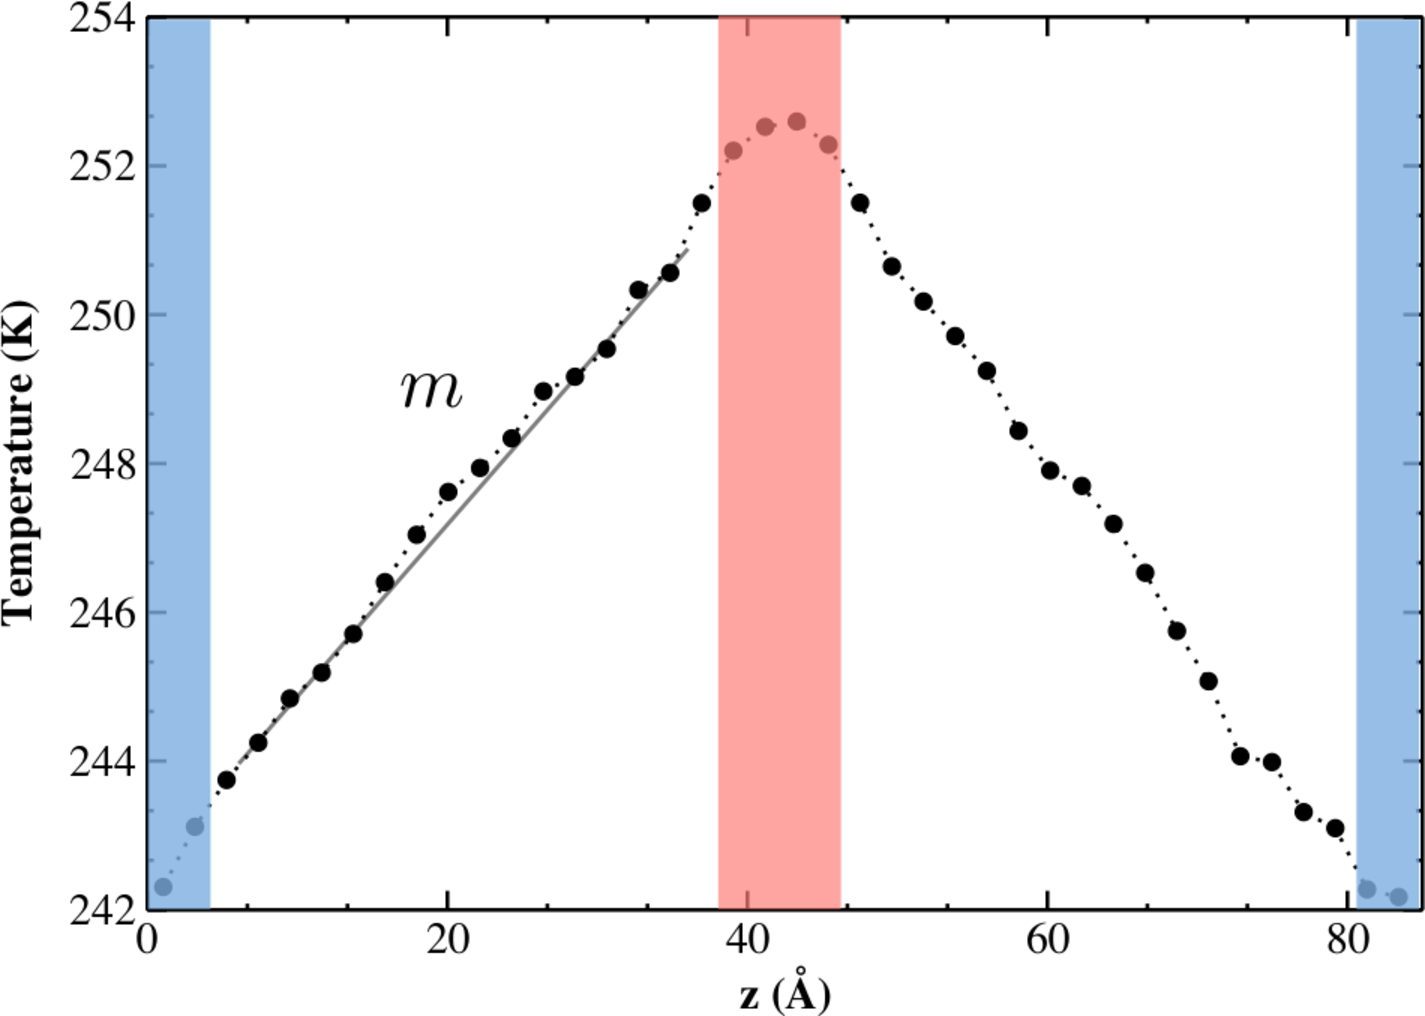
\includegraphics[scale=0.6]{figures/bulk-gradient.pdf}
    \caption{This figure is an example of the thermal gradient that develops in a bulk solvent system with a moderate flux. The red region is the ``hot'' bin and the two blue regions are the ``cold'' bins. The slope, $m$, that measures the temperature gradient is related to the thermal conductivity of the material, $\lambda$.}
    \label{fig:lambda-grad}
\end{figure}

In addition to finding the thermal conductivity of a material at different box lengths, the infinite box thermal conductivity of the material is extrapolated using the following equation:
\begin{equation}
    \frac{1}{\lambda_{\infty}}= \frac{1}{\lambda_L} +\frac{C}{L}
    \label{eq:lambda_inf}
\end{equation}
where $C$ is a constant and $L$ is the length of the simulation box in the z-direction.\cite{Hannah2015} 

\section{Results and Discussion}
A prediction using Eq. \ref{eq:composite} for a simple array of \ce{Au144PET60} particles can be made using separate simulations of each of the components of the system.
The bulk gold conductivity is compared to a previous study looking at gold particles in an array. 
Ultimately, as found in previous work by Zanjani \textit{et al.}\cite{Zanjani2014} and Ong \textit{et al.}\cite{Ong:2014yq}, the volume fraction of the array occupied by the particles is the essential piece of the predictive equation.
While the interfacial details is of lesser importance to the prediction of the thermal conductivity of the material, the two solvents do alter heat transport out of the nanoclusters.
This confirms previous findings regarding solvent penetration being paramount to thermal transport.
In the following sections, each of the individual components of the Hasselman and Johnson equation, as well as the overall prediction will be presented.
Additionally, thermal conductivity of the arrays will be discussed in comparison to the predicted results.

\subsection{Bulk Solvent and Bulk Gold Conductivity}
For the bulk dichloromethane and toluene solvent simulations, both were projected to infinite system size thermal conductivity using Eq \ref{eq:lambda_inf}. 
As seen in Fig. \ref{fig:inverselambda}, the box length projections of thermal conductivity is necessary for the dichloromethane solvent.
While projection to an infinite box size using Eq. \ref{eq:lambda_inf} is not required by the data for toluene and liquid gold.

The thermal conductivity of the dichloromethane from the projection to an infinite box and the thermal conductivity average of the toluene boxes are shown in Fig. \ref{fig:lambda-bulk}.
The infite box thermal conductivity of dichloromethane is 0.1084 $\pm$ 0.0021 W/mK and the conductivity of toluene is averaged to be 0.1082 $\pm$ 0.0054 W/mK.
If composition of the array is primarily solvent, the Hasselman and Johnson equation will therefor give nearly the same conductivity for the arrays.
It is important to note that the applied flux was small enough so that the density of the solvent across the simulation box was uniform.

\begin{figure}[h]
    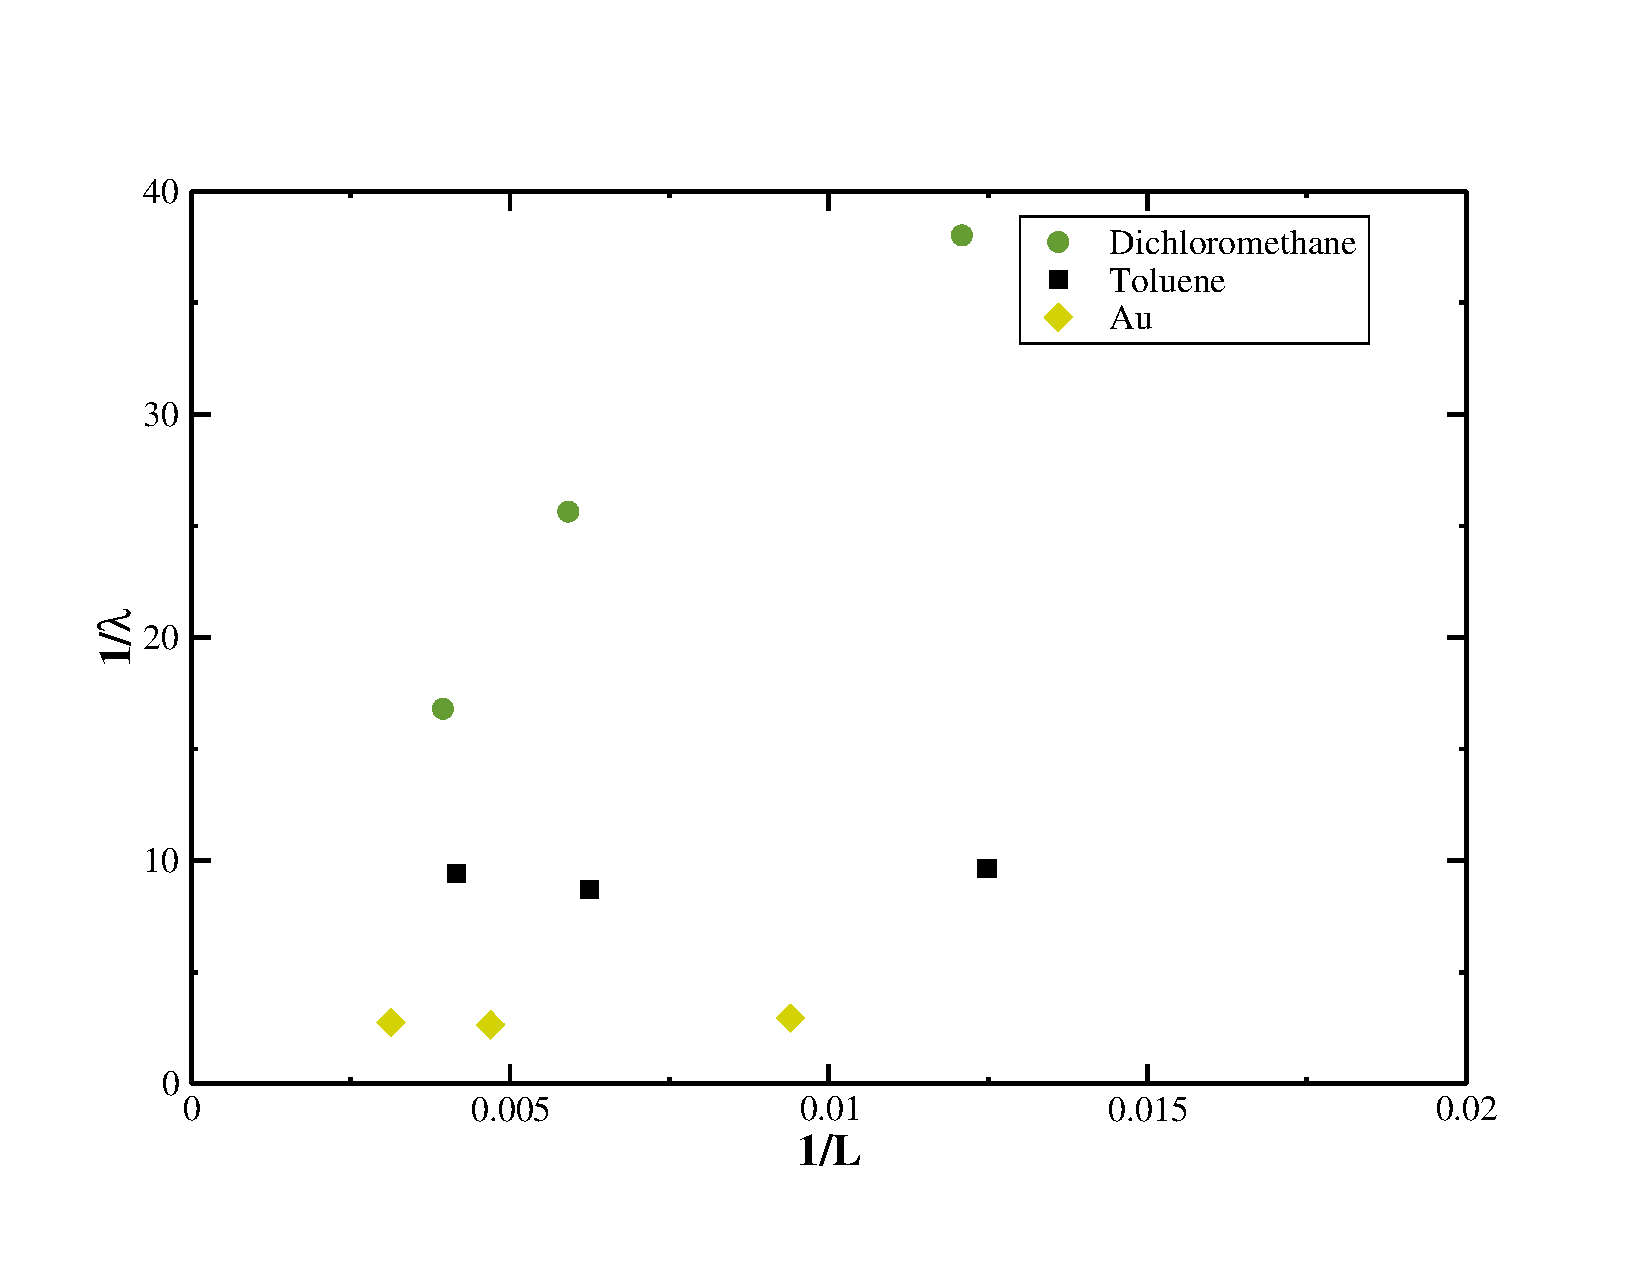
\includegraphics[scale=0.5]{figures/inverselambda-solvent.pdf}
    \caption{ Parameters to Eq. \ref{eq:lambda_inf} for bulk simulations of dichloromethane (green circles), toluene (black squares), and liquid gold (yellow diamonds). The y-axis, $\lambda$ is in units of W/mK. The x-axis, $L$ is in \AA.}
    \label{fig:inverselambda}
\end{figure}

%\begin{figure}[h]
%    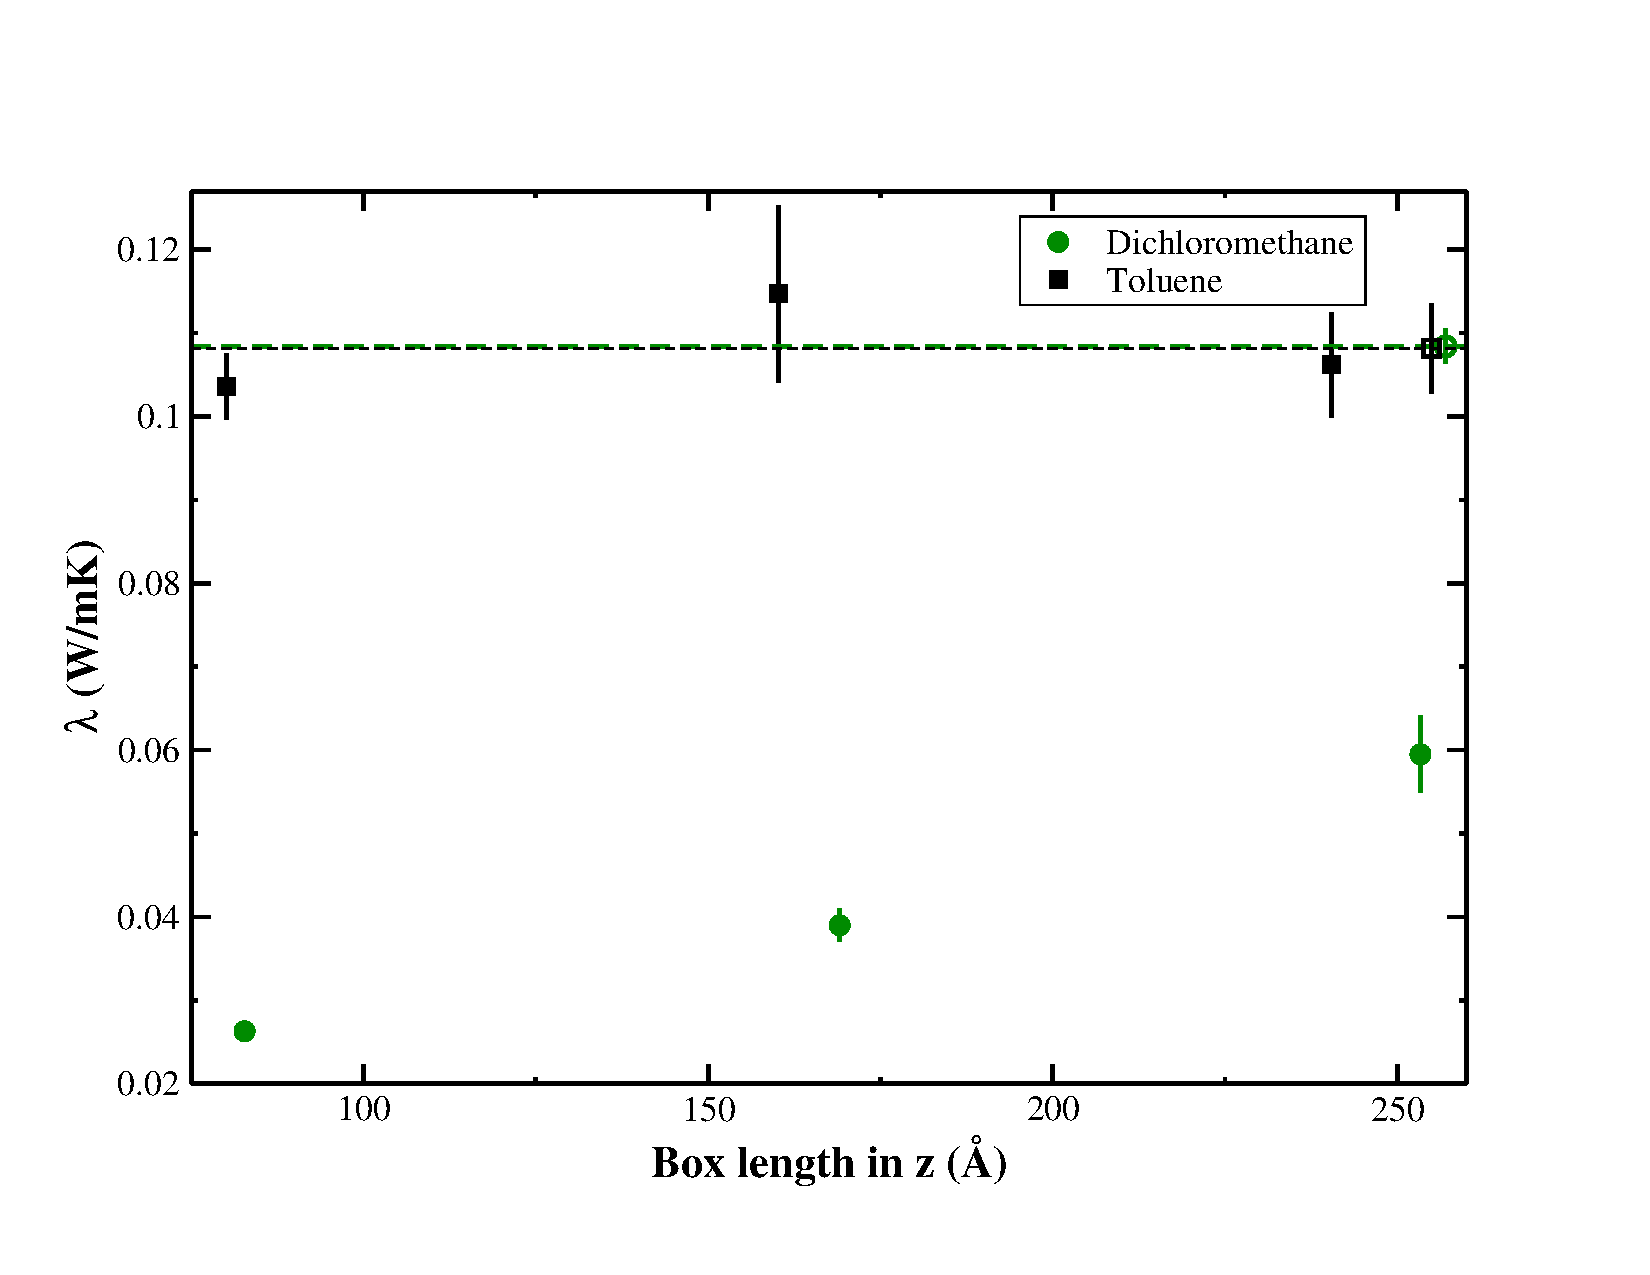
\includegraphics[scale=0.5]{figures/lambda-bulk.pdf}
%    \caption{ Bulk solvent $\lambda$ as a function of simulation box length in z displays the trend in dichloromethane with increasing box size. The dashed lines and open symbols are the projected $\lambda_{\infty}$ for dichloromethane and the average value for toluene.}
%    \label{fig:lambda-bulk}
%\end{figure}

The bulk gold simulations are essential to finding $\lambda_p$. Previous work from Ong \textit{et al.}\cite{Ong:2014yq} used bulk gold thermal conductivity of 1.8 $\pm$ 0.3 W/mK from simulations of a bulk `fcc' gold at 300 K for simulations of a gold nanocrystal array.
Their value will be compared to the conductivity of a bulk gold simulation at 1500 K, pass the melting point of the gold in QSC.
QSC has a size dependent melting temperature and previous particles of slightly larger radius have been shown to display liquid like structures.\cite{Stocker2016}
Experimentally, particles with $N<219$ have been seen with an approximate melting temperature of 500 K.\cite{Ercolessi1991}
Additionally, it was proposed through extrapolating melting temperatures vs. diameter, that the \ce{Au144PET60} cluster (with a diameter of $\approx$ 18 \AA) would melt at approximately 600 K.\cite{Buffat1976}
Hence the high temperature simulations of 100 \AA, 200 \AA, and 300 \AA\ box length in z were computed and displayed $\lambda_p$ = 0.3787 $\pm$ 0.02 W/mK.
The lower conductivity makes some sense; when the gold melts, the ballistic phonons traveling through the gold lattice are disrupted, and the transmission of the phonons decreases.

\subsection{Interfacial Thermal Conductivity}
The interfacial thermal conductance, $G$, for the particles was found in both solvents.
%In an attempt to force the interfacial density of toluene in these single particle to more closely match the experimental bulk density, 
The solvent outside of the interfacial region of the system is about twice the density of bulk toluene to maintain the solvent near the interface at a normal density.
This was not an issue with the dichloromethane systems. 
Across the staple motif the thermal conductivity to the toluene was 11.37 $\pm$ 0.66 MW/m$^2$K, while to dichloromethane $G$ = 74.73 $\pm$ 4.28 MW/m$^2$K.

%POSSIBLY SOMETHING ABOUT THE INTERPENETRATION OF SOLVENT
\subsection{Prediction of Array Thermal Conductivity}
Along with the components of the equation for bulk thermal conductivity, $v_p$, the partial volume of the \ce{Au144PET60} particles in the array is required to predict array conductivity.
The partial volume is approximated through the effective radius of the particles, which is taken from the average of the radius for only the outermost gold atoms and the radius of the total particle including the staple motif.
This approximations gives a partial volume of 22.5\%.
A total particle volume which includes all the ligand layer, allows for solvent to penetrate into the particle and would overestimate the volume fraction of the particles for a $v_p = 47.7\%$.

Using the parameters calculated in this study, $\lambda_s$, $\lambda_p$, $G$, and $v_p$, Eq.\ref{eq:composite} used to predict the thermal conductivity of the array.
Using the bulk gold thermal conductivity reported by Ong \textit{et al.} for gold at 300 K and the value calculated here for 1500 K, the array thermal conductivity can be found in Table \ref{tab:predition}.
As seen in previous work,\cite{Ong:2014yq, Liu2015, Zanjani2014} the volume fraction of the particles is the main determining factor of the thermal conductivity. 
With the small $v_p$, $\lambda_s$ dominates $\lambda_e$, thus there is a similar conductivity for the array across solvent (since $\lambda_s$ is nearly the same for the bulk thermal conductivity) and $\lambda_p$.

\begin{table}[]
    \centering
    \begin{tabular}{c|c|c}
    \toprule
         &$\lambda_p^{1500 K}$ & $\lambda_p^{300 K}$  \\
         \hline
         $\lambda_e^{DCM}$& 0.1184& 0.1256\\
         $\lambda_e^{Toluene}$ & 0.1182 & 0.1254 \\
         \bottomrule
    \end{tabular}
    \caption{The Hasselman and Johnson prediction for thermal conductivity of the \ce{Au144PET60} array using the gold thermal conductivity at 1500 K and 300 K. The array prediction for dichloromethane and toluene using the bulk thermal conductivity of each solvent.}
    \label{tab:predition}
\end{table}

\subsection{Simulations of Arrays}
Preliminary results of the smallest arrays displays behavior that indicate that Eq. \ref{eq:composite} might be missing a more complex component of the system.
The smallest system (2x2x2) in dichloromethane was simulated to find $\lambda = 0.0307 \pm 0.009$ W/mK. 
This is far below the predicted value of 0.1184 W/mK, but the dichloromethane bulk solvent displayed length-dependent thermal conductivity.
Therefore, it is possible that with larger arrays in dichloromethane, a length-dependent thermal conductivity will be extrapolated. 
Additionally, it is possible that the dichloromethane in the arrays behaves differently than the bulk fluid and might have thermal properties more similar to a confined liquid.

\section{Conclusions}
While there is still more that needs to be explained in the nanoarrays of the \ce{Au144PET60} particles, interesting results have been found using the Hasselman and Johnson model. 
To use the model, each component of the nanoarray was simulated to find the relevant thermal transport property. 
As found in previous works, the main component of the Eq. \ref{eq:composite} is $v_p$. 
The geometric arrangement of the array is the most important aspect contributing to the thermal conductance of the material.

In finding the component pieces of Eq. \ref{eq:composite}, interest results were found for the pure liquid simulations and the interfacial thermal conductivity of the particle.
The two solvents do not have the same length-dependent behavior thermal transport properties. This suggests interesting differences for the density dependent thermal conductivity in liquids.
Similarly, the large difference in $G$ between the two solvent interfaces with the particle, brings about questions of what is most important in ligand--solvent design.



%%%%%%%%%%%%%%%%%%%%%%%%%%%%%%%%%%%%%%%%%%%%%%%%%%%%%%%%%%%%%%%%%%%%%%%%%%%%%%%%%%%
%		CHAPTER 5 -- Conclusion
%%%%%%%%%%%%%%%%%%%%%%%%%%%%%%%%%%%%%%%%%%%%%%%%%%%%%%%%%%%%%%%%%%%%%%%%%%%%%%%%%%%
\chapter{CONCLUSION}\label{chap:conclusion}
In this dissertation, applications of Reverse Non-Equilibrium Molecular Dynamics and the Langenvin Hull method were applied to systems containing gold nanoparticles. Gold nanoparticles have well characterized optical properties, but less-well explored thermal properties, which are typically important in the period after electronic excitation. The simulations in previous chapters explored the effect of ligand rigidity, gold particle morphology, and staple motifs in nanoarrays using molecular dynamics.

Understanding how the capping agent, or ligand, on gold nanoparticles interacts with the particle and solvent environment is essential to predicting behavior of nanoparticles in a given system. Adding rigidity to the ligand layer changed the penetration accessibility of the interfacial solvent. With a more rigid ligand, the solvent generally has an increased penetration into the ligand layer. This leads to a stronger vibrational overlap of the ligand and solvent, and thus more rapid thermal transport. Additionally, the addition of the ligand layer aids interfacial thermal conductivity. The sulfur on the thiolate ligand acts as a conduit for heat from the particle to the solvent.

Though the ligand layer is experimentally interesting and has promising characteristics for tailoring a nanoparticle for desired thermal and optical properties, a bare particle gives insight to how the morphology of the gold particle affects thermal transport.
From simulations of spheres, cuboctahedra, and icosahedra; the surface structure of the gold particle is essential to thermal transport from bare particles.
Furthermore, work in chapter 3 displayed that the underlying lattice carries important information on the low frequency phonon modes. 

In an effort examine both the ligand and undercoordination of gold atoms at the surface within the same system, chapter 4 investigates the effect of the staple motif on \ce{Au144PET60} nanoclusters.
The nanoparticles were examined in two different solvents; one polar and one non-polar; in single particle systems and in nanoarrays.
While the array systems have so far yielded inconclusive results, the single particle systems display interesting behavior with respect to the ligand/solvent interactions. 
While the staple motif might increase the conductivity through the undercoordinated gold atoms in the ligand, the solvent is ultimately the limiting factor in thermal transport. 
Additionally, the solvent thermal conductivity due to the partial volume becomes the dominating factor in the predictive equation for thermal conductivity through an array of \ce{Au144PET60} particles.

In the future, biologically relevant systems would be an interesting avenue to explore. 
With the new polarizable metal model (DR-EAM), being developed in the group, the gold substrate would be able to more appropriately interact with polar molecules.
Thus, a good starting system would be a gold slab displaying (111) facets in water.

To systematically determine how polarization affects thermal conductivity in a simple gold/water system, each of the components should be tested individually. Therefore the following systems should be examined: \ce{H2O}/gold (with and without polarization) and fluctuating-charge \ce{H2O}/gold (with and without fluctuating charge).
If the polarization of the gold and water effects the the interfacial thermal conductivity of the system, moving forward with biologically relevant systems would be the next course of action.
Various interesting ligands such as: thiolated PEG, citrate, Cetyl trimethylammonium bromide(CTAB), and different carboxylic acid moieties; could be tested on planar and spherical systems. The differences in these could then be identified to tailor nanoparticles for different thermal needs.

In addition to the further work needed in the gold nanoparticle systems, the trend in pure solvents would be an interesting avenue to explore.
In chapter 4, the two solvents (dichloromethane and toluene) had very different thermal conductivity values at the three box lengths simulated but had the same infinite box length bulk thermal conductivity.
Dicholormethane, with a density of $\approx$ 2x that of toluene, had a clear box length dependence, while toluene did not. 
It would be interesting to follow these simulations with a range of different common solvents, with known thermal conductivities, and look not only at the box dependences but a normal mode analysis.
In the more dense fluids it is possible that the imaginary frequencies would be more heavily populated, leading to higher bulk thermal conductivities.

The work presented in this work has shown significant progress in identifying the trends that are important for controlling the thermal properties of gold nanoparticles. Moving forward, work with polarizable force fields, biologically relevant ligands and capping agents, and elucidating trends in solvent thermal conductivity would move nanoparticle design forward.


%%%%%%%%%%%%%%%%%%%%%%%%%%%%%%%%%%%%%%%%%%%%%%%%%%%%%%%%%%%%%%%%%%%%%%%%%%%%%%%%%%%
%%%%%%%%%%%%%%%%%%%%%%%%%%%%%%%%%%%%%%%%%%%%%%%%%%%%%%%%%%%%%%%%%%%%%%%%%%%%%%%%%%%
%		UNNUMBERED CHAPTER
%%%%%%%%%%%%%%%%%%%%%%%%%%%%%%%%%%%%%%%%%%%%%%%%%%%%%%%%%%%%%%%%%%%%%%%%%%%%%%%%%%%
% \unnumchapter{FEATURES OF FORMATTING IN THIS EXAMPLE FILE}
% The \unnumchapter command allows you to include an unnumbered chapter as part of
% the main text before Chapter 1. It will appear in your table of contents, and you
% should have at most one such chapter (although nothing in the class file will
% prevent you from creating more).

%%%%%%%%%%%%%%%%%%%%%%%%%%%%%%%%%%%%%%%%%%%%%%%%%%%%%%%%%%%%%%%%%%%%%%%%%%%%%%%%%%%
%		APPENDIX
%%%%%%%%%%%%%%%%%%%%%%%%%%%%%%%%%%%%%%%%%%%%%%%%%%%%%%%%%%%%%%%%%%%%%%%%%%%%%%%%%%%
%\appendix
%\include{Chapters/appendix1}
%\include{Chapters/structuralAppendix}
%\include{Chapters/dynamicAppendix}
%%%%%%%%%%%%%%%%%%%%%%%%%%%%%%%%%%%%%%%%%%%%%%%%%%%%%%%%%%%%%%%%%%%%%%%%%%%%%%%%%%%
%		BACK STUFF
%%%%%%%%%%%%%%%%%%%%%%%%%%%%%%%%%%%%%%%%%%%%%%%%%%%%%%%%%%%%%%%%%%%%%%%%%%%%%%%%%%%

% % comment out the following three lines
% if using chapter-wise bibliography

 \backmatter
 
%\bibliographystyle{nddiss2e}
%\bibliographystyle{nddiss2enoarticletitles}
\bibliographystyle{achemso}
%\bibliographystyle{abbrvnat} 
\bibliography{Neidhart_Thesis} 
 
 
\end{document}

\endinput
